%%%%%%%%%%%%%%%%%%%%%%%%%%%%%%%%%%%%%%%%%%%%%%%%%%%%%
%% File: main.tex
%% Author: Evangelos Stamos (estamos@e-ce.uth.gr)
%% Last update: February, 2021
%% Description: Provides an example of a Diploma Thesis 
%% using the ntua-thesis pdfLaTeX class.
%%
%% Character encoding: UTF-8
%%%%%%%%%%%%%%%%%%%%%%%%%%%%%%%%%%%%%%%%%%%%%%%%%%%%%
%
%
%%%%%%
% 1. use the "modern" or "classic" option to switch between 
% a modern or classic font, respectively.
%
% 2. add/remove the "hyperref" option to enable/disable hyperlinks:
% (remember to remove auxiliary files after adding/removing 
% the "hyperref" option).
%
% 3. add/remove the "printer" option to typeset a printer-friendly 
% (grayscale)/color version of the thesis.
%
% 4. use the "watermark" option to indicate that this is not an actual
% thesis.
%
% 5. use the "histinit" option to enable "historiated initials".
% (If used, all chapter initials declared by the \InitialCharacter{}
% macro are enlarged. If omitted, arguments of \InitialCharacter{}
% are typeset as normal text.)
%
% 6. use the "plain" option to disable tikz graphics in title page
% and part/chapter headers (might help to avoid compilation timeouts).
% Note that "plain" disables CD label and CD cover creation.
%
% 7. use the "noindex" option to (hopefully) avoid compilation timeouts
% when compiling online (disables index generation - note that "\indexGR",
% "\indexEN" invocations need not be removed when toggling this option).
%
% 8. activate the "newlogo" option to use the new official Logo.
%
%%%%%%%%%%%%%%%%%%%%%%%%%%%%%%%%%%%%%%%%%%%%%%%%%%%%%%%%%%%%%%%%%%%%%%%%%%%%%%%
%
\documentclass[modern,hyperref,watermark,histinit,noindex,plain,newlogo]{ntua-thesis}
% \usepackage[greek,english]{babel}
% \usepackage[LGR,T1]{fontenc}
% \usepackage{alphabeta}
\usepackage{bm}
\usepackage{pgfplots}
\pgfplotsset{compat=1.18}
\usepackage{subcaption}
\usepackage{booktabs}     % for \toprule, \midrule, \bottomrule in tables
\usepackage{xcolor}       % for custom color definitions

\usepackage{placeins}  % FOR SETTING A BARRIER SO FIGURES DO NOT GO TO THE WRONG SECTIONS - USAGE: \FloatBarrier before the next section

% For tiks plots

% =====================================================================
%  Preamble additions for the distillation framework diagrams
%  (Chapter 6).  Add this block ONCE to the thesis preamble, after the
%  existing \usepackage{xcolor}/pgfplots lines.
% =====================================================================
\usepackage{tikz}
\usetikzlibrary{positioning,fit,backgrounds,arrows.meta,calc,shapes.geometric}

% --- Colours --------------------------------------------------------
% colorExperiment / colorBaseline are also defined in chap7.tex for the
% result plots; repeating them here is harmless and guarantees the Ch.6
% figures compile regardless of \include order.
\definecolor{colorExperiment}{RGB}{0,84,159}   % NTUA deep blue -> student / trainable
\definecolor{colorBaseline}{RGB}{150,150,150}  % neutral gray   -> teacher / frozen
\definecolor{distill}{RGB}{178,34,34}          % firebrick      -> distillation signal
\definecolor{initclr}{RGB}{0,128,96}           % teal-green     -> offline weight init

% --- Shared TikZ styles for both diagrams ---------------------------
\tikzset{
  blk/.style={rounded corners=2pt,draw,align=center,font=\footnotesize,inner sep=4pt,minimum height=8mm},
  sblk/.style={blk,fill=colorExperiment!8,draw=colorExperiment!60},
  tblk/.style={blk,fill=black!5,draw=colorBaseline!90,text=black!55},
  stage/.style={blk,fill=black!3,draw=black!45},
  shallow/.style={line width=0.9pt},
  loss/.style={rounded corners=2pt,draw=distill!70,fill=distill!8,align=center,font=\footnotesize,inner sep=4pt,minimum height=8mm},
  tot/.style={rounded corners=2pt,draw=distill,fill=distill!12,align=center,font=\footnotesize\bfseries,inner sep=4pt,minimum height=9mm},
  ema/.style={rounded corners=2pt,draw=colorExperiment!60,fill=colorExperiment!6,align=center,font=\scriptsize,inner sep=3pt},
  io/.style={rounded corners=2pt,draw=black!50,fill=black!3,align=center,font=\footnotesize,inner sep=3pt},
  darr/.style={-{Latex[length=2mm]},dashed,distill,line width=0.8pt},
  farr/.style={-{Latex[length=2mm]},black!60,line width=0.7pt},
  sarr/.style={-{Latex[length=2mm]},colorExperiment!75,line width=0.8pt},
  tarr/.style={-{Latex[length=2mm]},black!55,line width=0.8pt},
  larr/.style={-{Latex[length=2mm]},distill!75,line width=0.8pt},
  vel/.style={-{Latex[length=2mm]},black!50,line width=0.6pt},
  iarr/.style={-{Latex[length=2.2mm]},initclr,line width=1.1pt},
  bp/.style={-{Latex[length=2.2mm]},dashed,colorExperiment,line width=0.9pt},
}

% --- Padlock glyphs (frozen vs. trainable) --------------------------
\newcommand{\lockclosed}[2]{\begin{scope}[shift={#1}]
  \fill[#2](-1.6mm,-1.4mm)rectangle(1.6mm,1.2mm);
  \draw[#2,line width=0.5pt](-1.0mm,1.2mm)arc(180:0:1.0mm)--(1.0mm,1.2mm);
  \fill[white](0,-0.1mm)circle(0.35mm);\end{scope}}
\newcommand{\lockopen}[2]{\begin{scope}[shift={#1}]
  \fill[#2](-1.6mm,-1.4mm)rectangle(1.6mm,1.2mm);
  \draw[#2,line width=0.5pt]
    (0.9mm,1.2mm) -- (0.9mm,2.3mm)
    arc(0:180:0.9mm);
  \fill[white](0,-0.1mm)circle(0.35mm);\end{scope}}
\end{scope}}

%
%%%%%%%%%%%%%%%%%%%%%%%%%%%%%%%%%%%%%%%%%%%%%%%%%%%%%%%%%%%%%%%%%%%%%%%%%%%%%%%
%
%
%%%%%%%%%%%%%%%%%%%%%%%%%%%%%%%%%%%%%%%%%%%%%%%%%%%%
%% THESIS INFO 
%%%%%%%%%%%%%%%%%%%%%%%%%%%%%%%%%%%%%%%%%%%%%%%%%%%%
%
% ΤΙΤΛΟΣ ΔΙΠΛΩΜΑΤΙΚΗΣ ΕΡΓΑΣΙΑΣ 
%
% Για εξαναγκασμένες αλλαγές γραμμής χρησιμοποιήστε "\\".
% Αν οι αλλαγές γραμμής πρέπει να είναι διαφορετικές στο εξώφυλλο σε σχέση 
% με το εσώφυλλο (σελ. 3), επαναλάβετε τον τίτλο του εξωφύλλου με τις 
% επιθυμητές αλλαγές γραμμής ως προαιρετικό όρισμα της εντολής \title.
%
% Παραδείγματα:
% 1. Όμοιος τίτλος σε εξώφυλλο και εσώφυλλο, με αυτόματες αλλαγές γραμμής:
%	    \title{Πρότυπο Σύστημα Ομότιμων Κόμβων Βασισμένο σε Σχήματα \en{RDF}}
% 2. Όμοιος τίτλος σε εξώφυλλο και εσώφυλλο, με αλλαγή γραμμής μετά τη λέξη
% "Σύστημα":
%	    \title{Πρότυπο Σύστημα \\ Ομότιμων Κόμβων Βασισμένο σε Σχήματα \en{RDF}}
% 3. Διαφορετικές αλλαγές γραμμής σε εξώφυλλο και εσώφυλλο. Στο εξώφυλλο 
% έχουμε αλλαγή γραμμής μετά τη λέξη "Σύστημα", ενώ στο εσώφυλλο η αλλαγή
% γραμμής ακολουθεί τη λέξη "Ομότιμων":
%	    \title[Πρότυπο Σύστημα \\ Ομότιμων Κόμβων Βασισμένο %
%           σε Σχήματα \en{RDF}]% (προαιρετικό όρισμα)
%           {Πρότυπο Σύστημα Ομότιμων \\ Κόμβων Βασισμένο σε %
%           Σχήματα \en{RDF}}% (υποχρεωτικό όρισμα)
%
	\title{Large Generative Model Distillation}
%%
%
%% -------------------------------------------------------------------
%% ΥΠΟΤΙΤΛΟΣ ΔΙΠΛΩΜΑΤΙΚΗΣ ΕΡΓΑΣΙΑΣ (προαιρετικός)
%
% Αν δεν υπάρχει υπότιτλος, τοποθετήστε τον χαρακτήρα του σχολίου "%"
% πριν από την εντολή \subtitle, ή αφήστε κενό το όρισμα της εντολής.
%
% Παράδειγμα:
%%	\subtitle{Μελέτη και υλοποίηση}
%
%% -------------------------------------------------------------------
%% ΤΟΥ/ΤΗΣ/ΤΩΝ
%
% "του" ή "της" ή "των", ανάλογα με το φύλο/αριθμό του σπουδαστή ή 
% των σπουδαστών
% Παράδειγμα:
%	\toutis{του}
	\toutis{\en{of}}
%
%% -------------------------------------------------------------------
%% ΟΝΟΜΑΤΕΠΩΝΥΜΟ ΣΠΟΥΔΑΣΤΗ ΣΤΑ ΕΛΛΗΝΙΚΑ (ΚΕΦΑΛΑΙΑ, ΓΕΝΙΚΗ ΠΤΩΣΗ)
%
% Για περισσότερους του ενός σπουδαστές, διαχωρίστε με ",".
% Παράδειγμα:
%	\authorNameCapitalGR{ΚΩΝΣΤΑΝΤΙΝΟΥ Δ. ΔΗΜΗΤΡΙΟΥ, ΓΕΩΡΓΙΟΥ Π. ΠΑΝΑΓΑΚΗ}
%	\authorNameCapitalGR{ΣΤΑΜΟΥ Φ. ΕΥΑΓΓΕΛΟΥ}
%
%% -------------------------------------------------------------------
%% ΟΝΟΜΑΤΕΠΩΝΥΜΟ ΣΠΟΥΔΑΣΤΗ ΣΤΗ ΛΑΤΙΝΙΚΗ ΜΟΡΦΗ (ΠΕΖΑ)
%
% Δηλώστε εδώ τυχόν ονοματεπώνυμα στη λατινική μορφή, αλλιώς αφήστε
% κενό το όρισμα.
% Για περισσότερους του ενός σπουδαστές, διαχωρίστε με ",".
% Παράδειγμα:
%	\authorNameEN{Albert Einstein, George W. Bush} 
	\authorNameEN{Yassin Ahmed} 
%
%% -------------------------------------------------------------------
%% ΟΝΟΜΑΤΕΠΩΝΥΜΟ ΣΠΟΥΔΑΣΤΗ ΣΤΑ ΕΛΛΗΝΙΚΑ (ΠΕΖΑ, ΟΝΟΜΑΣΤΙΚΗ ΠΤΩΣΗ)
%
% Για περισσότερους του ενός σπουδαστές, διαχωρίστε με ",".
% Αν τα ονοματεπώνυμα όλων των σπουδαστών είναι σε λατινική μορφή,
% αφήστε κενό το όρισμα.
% Παράδειγμα:
%	\authorNameGR{Κωνσταντίνος Δημητρίου, Γεώργιος Παναγάκης}
%	\authorNameGR{Ευάγγελος Στάμος}
%
%% -------------------------------------------------------------------
%% ΟΝΟΜΑΤΕΠΩΝΥΜΟ ΕΠΙΒΛΕΠΟΝΤΑ ΚΑΘΗΓΗΤΗ
% 
	\supervisor{Athanasios Voulodimos}
%
%% -------------------------------------------------------------------
%% ΤΙΤΛΟΣ ΕΠΙΒΛΕΠΟΝΤΑ ΚΑΘΗΓΗΤΗ
%
	\supervisorTitle{Assistant Professor NTUA}
%
%% -------------------------------------------------------------------
%% ΕΠΙΒΛΕΠΩΝ/ΕΠΙΒΛΕΠΟΥΣΑ
%
% "Επιβλέπων" ή "Επιβλέπουσα", ανάλογα με το φύλο του 
% Επιβλέποντα Καθηγητή
	\supervisorMaleFemale{Supervisor}
%
%% -------------------------------------------------------------------
%% ΤΟΠΟΣ/ΜΗΝΑΣ/ΕΤΟΣ ΕΚΔΟΣΗΣ
%
	\thesisPlaceDate{Athens, May 2026}
%
%% -------------------------------------------------------------------
%% ΤΟΠΟΣ/ΜΗΝΑΣ/ΕΤΟΣ ΣΥΓΓΡΑΦΗΣ (Εμφανίζεται στη σελίδα των ευχαριστιών,
%% αν υπάρχει).
%
	\ackPlaceDate{Athens, May 2026}
%
%% -------------------------------------------------------------------
%% ΗΜΕΡΟΜΗΝΙΑ ΕΞΕΤΑΣΗΣ
%
	\examinationDate{22nd July 2026}
%% -------------------------------------------------------------------
%% ΗΜΕΡΟΜΗΝΙΑ ΔΗΛΩΣΗΣ ΠΕΡΙ ΜΗ ΛΟΓΟΚΛΟΠΗΣ
%
	\declarationDate{22nd July 2026}
%
%% -------------------------------------------------------------------
%% ΕΤΟΣ COPYRIGHT
%
	\copyrightYear{2026}
%
%% -------------------------------------------------------------------
%% ΟΝΟΜΑΤΕΠΩΝΥΜΟ 1ου ΕΞΕΤΑΣΤΗ
%
	\firstExaminer{Georgios Stamou}
%
%% -------------------------------------------------------------------
%% ΤΙΤΛΟΣ 1ου ΕΞΕΤΑΣΤΗ
%
	\firstExaminerTitle{Professor NTUA}
%
%% -------------------------------------------------------------------
%% ΟΝΟΜΑΤΕΠΩΝΥΜΟ 2ου ΕΞΕΤΑΣΤΗ
%
	\secondExaminer{Andreas-Georgios Stafylopatis}
%
%% -------------------------------------------------------------------
%% ΤΙΤΛΟΣ 2ου ΕΞΕΤΑΣΤΗ
%
	\secondExaminerTitle{Professor NTUA}
%%
%%
%%%%%%%%%%%%%%%%%%%%%%%%%%%%%%%%%%%%%%%%%%%%%%%%%%%%%%%%%%%%%%%%%%%%%%
%% THESIS COLORS: 
%%%%%%%%%%%%%%%%%%%%%%%%%%%%%%%%%%%%%%%%%%%%%%%%%%%%%%%%%%%%%%%%%%%%%%
%%
%% Χρώμα εξωφύλλου - κεφαλαίων
	\chaptercolor{gray!50!brown}
%%
%% Χρώμα παραρτημάτων
	\appendixcolor{brown!60!orange}
%%
%% Χρώμα υπερσυνδέσμων (αν έχει ενεργοποιηθεί η επιλογή "hyperref")
    \hyperlinkcolor{blue}
%%
%% Χρώμα τίτλου εργασίας στο εξώφυλλο (αν δεν έχει ενεργοποιηθεί 
%% η επιλογή "plain")
    \titlecolor{white}
%%
%% Χρώμα υποβάθρου (φόντου) τίτλου εργασίας στο εξώφυλλο (αν δεν έχει 
%% ενεργοποιηθεί η επιλογή "plain")
    \titlebackgroundcolor{gray!60!brown}  
%%
%%
%%%%%%%%%%%%%%%%%%%%%%%%%%%%%%%%%%%%%%%%%%%%%%%%%%%%%%%%%%%%%%%%%%%%%%
%% COVER PAGE IMAGE: 
%%%%%%%%%%%%%%%%%%%%%%%%%%%%%%%%%%%%%%%%%%%%%%%%%%%%%%%%%%%%%%%%%%%%%%
%%
%% Εικόνα εξωφύλλου (προαιρετική)
%% Στην περίπτωση κατά την οποία δεν είναι επιθυμητή η εισαγωγή εικόνας στο εξώφυλλο,
%% διαγράψτε την εντολή \coverpageimage, ή μετατρέψτε την σε σχόλιο (με "%")
%%
%% Σύνταξη:
%%          \coverpageimage{συντελεστής μεγέθυνσης}{όνομα αρχείου εικόνας [πλήρης διαδρομή]}
%%      ή
%%          \coverpageimage[tikz]{συντελεστής μεγέθυνσης}{εντολές TikZ}
%%          (στις εντολές μπορούν να περιλαμβάνονται και δηλώσεις \usetikzlibrary, κ.λπ.)
%%      
%% Παραδείγματα:
%%      - Χρήση εικόνας από το αρχείο "figures/rdf.png" με συντελεστή μεγέθυνσης 0.8:
%%          \coverpageimage{0.8}{figures/rdf.png}
%%      - Χρήση εικόνας TikZ με συντελεστή μεγέθυνσης 0.5:
%%          \coverpageimage[tikz]{0.5}{
%%              \draw[thick, gray] \foreach \x in {18,90,...,306} {
%%                  (\x:4) node{} -- (\x+72:4)
%%                  (\x:4) -- (\x:3) node{}
%%                  (\x:3) -- (\x+15:2) node{}
%%                  (\x:3) -- (\x-15:2) node{}
%%                  (\x+15:2) -- (\x+144-15:2)
%%                  (\x-15:2) -- (\x+144+15:2)
%%              };
%%          }
%%
     \coverpageimage{0.8}{figures/rdf.png}
%%
%%%%%%%%%%%%%%%%%%%%%%%%%%%%%%%%%%%%%%%%%%%%%%%%%%%%%%%%%%%%%%%%%%%%%%
%
% add custom hyphenation rules here
%\hyphenation{ο-ποί-α} 
%
%%%%
%
%
%%%%
\begin{document}

\maketitle

\beginfrontmatter

\renewcommand{\partname}{Part}
\renewcommand{\chaptername}{Chapter}
\captionsetup[figure]{labelfont={bf},name={Figure},labelsep=period}
\renewcommand{\contentsname}{Table of Contents}
\renewcommand{\listfigurename}{List of Figures}
\renewcommand{\listtablename}{List of Tables}
\renewcommand{\listillustrationname}{List of Images}
\renewcommand{\appendixname}{\Appendix}
\renewcommand{\bibname}{Bibliography}
\captionsetup[table]{labelfont={bf},name={Table},labelsep=period}

% Περίληψη
	\selectlanguage{greek}
\begin{abstract}

Τα μοντέλα διάχυσης έχουν αναδειχθεί ως το επικρατέστερο παράδειγμα για τη
σύνθεση εικόνων υψηλής πιστότητας, ωστόσο η ανάπτυξή τους σε περιβάλλοντα
περιορισμένων υπολογιστικών πόρων παραμένει δυσχερής λόγω του υψηλού
υπολογιστικού κόστους των αρχιτεκτονικών μεγάλης χωρητικότητας. Η παρούσα
διπλωματική εργασία διερευνά την εφαρμογή της απόσταξης γνώσης σε μοντέλα
διάχυσης χώρου εικονοστοιχείων ως μηχανισμό βελτίωσης της ποιότητας παραγωγής
ενός συμπαγούς μοντέλου-μαθητή, χωρίς τροποποίηση της αρχιτεκτονικής του κατά
την εξαγωγή συμπερασμάτων ή του υπολογιστικού του αποτυπώματος --- έναν στόχο
ορθογώνιο προς το ευρέως μελετημένο πρόβλημα της επιτάχυνσης δειγματοληψίας.
Στο πλαίσιο ενός σχήματος δασκάλου--μαθητή με παγωμένες παραμέτρους δασκάλου,
βασισμένου σε αρχιτεκτονική Vision Transformer εκπαιδευμένη με αντικειμενική
συνάρτηση αντιστοίχισης ροής, προτείνουμε και αξιολογούμε συστηματικά ένα ενιαίο
σχήμα απόσταξης που συνδυάζει ευθυγράμμιση ενδιάμεσων χαρτών χαρακτηριστικών,
μεταφορά προτύπων προσοχής, στάθμιση απωλειών με επίγνωση του βήματος χρόνου,
και αρχικοποίηση βαρών από τον δάσκαλο. Πειράματα σε σημεία αναφοράς παραγωγής
εικόνων καταδεικνύουν ότι το προτεινόμενο πλαίσιο μπορεί σε κάποιες περιπτώσεις να βελτιώσει την ποιότητα παραγωγής του μοντέλου-μαθητή σε σχέση με ένα αντίστοιχο μοντέλο εκπαιδευμένο από την αρχή υπό πανομοιότυπο υπολογιστικό προϋπολογισμό, επικυρώνοντας την απόσταξη γνώσης ως αποτελεσματική στρατηγική βελτίωσης ποιότητας για συμπαγή
μοντέλα διάχυσης.

   \begin{keywords}
      Μοντέλα Διάχυσης, Απόσταξη Γνώσης, Αντιστοίχιση Ροής,
      Παραγωγή Εικόνων, Απόσταξη Χαρακτηριστικών, Μεταφορά Προσοχής
   \end{keywords}
\end{abstract}


\selectlanguage{english}

\selectlanguage{english}
\begin{abstracteng}

Diffusion models have emerged as the dominant paradigm for high-fidelity image
synthesis, yet their deployment in resource-constrained settings remains impeded by
the substantial computational cost of large-capacity architectures. This thesis
investigates the application of knowledge distillation to pixel-space diffusion models
as a mechanism for improving the generative quality of a compact student model,
without modifying its inference-time architecture or computational footprint --- an
objective orthogonal to the well-studied problem of sampling acceleration. Operating
within a frozen teacher--student framework built upon a Vision Transformer backbone
trained with a flow-matching objective, we propose and systematically evaluate a
unified distillation scheme that combines intermediate feature map alignment,
attention pattern transfer, timestep-aware loss weighting, and teacher-derived weight
initialisation. Experiments on image generation benchmarks demonstrate that the
proposed framework under specific configurations can improve the generative quality of the student model
relative to a matched baseline trained from scratch under an identical computational
budget, validating knowledge distillation as an effective quality-boosting strategy for
compact diffusion models.

   \begin{keywordseng}
      Diffusion Models, Knowledge Distillation, Flow Matching, Vision Transformers,
      Image Generation, Feature Distillation, Attention Transfer
   \end{keywordseng}
\end{abstracteng}

% Αφιέρωση
	\thesisDedication{to my parents}
% Ευχαριστίες
	%%%%%%%%%%%%%%%%%%%%%%%%%%%%%%%%%%%%%%%%%%%%%%%%%%%%%%%%%%%%%%%%%
%%
%% use the starred version of the "acknowledgements" environment
%% to omit signatures from this section, e.g.:
%% \begin{acknowledgements*} ... \end{acknowledgements*}
%% 
%%%%%%%%%%%%%%%%%%%%%%%%%%%%%%%%%%%%%%%%%%%%%%%%%%%%%%%%%%%%%%%%%
\begin{acknowledgements}
This thesis would not have been possible without the guidance and support of several people to whom I owe my sincere gratitude.

First, I would like to thank my supervisor, Professor Athanasios Voulodimos, for his trust in assigning me this topic.

I am especially grateful to Nikos Spanos, whose day-to-day collaboration was invaluable. His constant availability, creative ideas, and genuine enthusiasm for the subject made the research process both rigorous and enjoyable.

Finally, and most deeply, I wish to thank my parents, my family, and my friends. Their unwavering support and encouragement throughout my years at NTUA have meant more than words can express.

\end{acknowledgements}

% Πίνακας Περιεχομένων
	\tableofcontents
% Κατάλογος Σχημάτων
	\listoffigures
% Κατάλογος Πινάκων
	\listoftables
	
\beginmainmatter

%%%%%%%%%%%%%%%%%%%%%%%%%%%%%%%%%%%%%%%%%%%%%%%%%%%%%
%% INCLUDE YOUR CHAPTERS/SECTIONS HERE
%%

    
% Εισαγωγή
    \selectlanguage{greek}
\chapter{Εκτεταμένη Περίληψη στα Έλληνικα}
Introduction content . . .
\selectlanguage{english}

	\include{body_matter/intro}
% Μέρη/Κεφάλαια

	\chapter{Generative Models for Image Generation}
\label{chap:generative_models}

One of the most active and important areas of current machine learning research is the study of generative models. Unlike discriminative models, which
learn to map inputs to labels, generative models aim to learn the underlying
probability distribution of a dataset so that novel, realistic samples can be
synthesized. The capacity to model complex, high-dimensional distributions has
profound implications for image synthesis, data augmentation, representation
learning, and scientific simulation, among many other domains. The main families of deep generative models are comprehensively explored in this chapter, which examines their development from early probabilistic methods to current score-based and flow-based techniques.

% -------------------------------------------------------------------

\section{Overview of Deep Generative Models}
\label{sec:overview_generative}

A generative model is formally defined as a parametric approximation
$p_\theta(\mathbf{x})$ to an unknown data distribution $p_{\text{data}}(\mathbf{x})$,
where $\mathbf{x} \in \mathbb{R}^d$ and $\theta$ denotes the learnable parameters.
The central objective is to choose $\theta$ such that $p_\theta$ is, in some
well-defined sense, close to $p_{\text{data}}$. In practice, this closeness is
quantified by a divergence or distance measure — most commonly the
Kullback--Leibler (KL) divergence, the Jensen--Shannon divergence, or an
integral probability metric such as the Wasserstein distance
\cite{villani2009optimal}.

The history of statistical generative modeling predates the deep learning era,
encompassing classical approaches such as Gaussian mixture models, restricted
Boltzmann machines, and deep Boltzmann machines. However starting in the early 2010s, a significant change in the capabilities of generative models was brought about by the combination of large-scale datasets, advanced GPU hardware, and expressive neural network architecture.

Four major families can be used to classify modern deep generative models while also in Figure~\ref{fig:generative_taxonomy} there is an alternative categorization:
\begin{enumerate}
    \item \textbf{Variational Autoencoders (VAEs)} \cite{kingma2013auto,
    rezende2014stochastic}, which optimise a tractable lower bound on the
    log-likelihood through amortised variational inference;
    \item \textbf{Generative Adversarial Networks (GANs)} \cite{goodfellow2014generative},
    which frame generation as a two-player minimax game between a generator
    and a discriminator;
    \item \textbf{Diffusion and Score-Based Models}
    \cite{ho2020denoising, song2021scorebased}, which learn to reverse a
    stochastic noising process defined over a continuous time horizon; and
    \item \textbf{Normalising Flows and Flow Matching} \cite{chen2018neural,
    lipman2022flow}, which construct an invertible, differentiable mapping
    between a simple base distribution and the data manifold.
\end{enumerate}

\begin{figure}[ht]
    \centering
    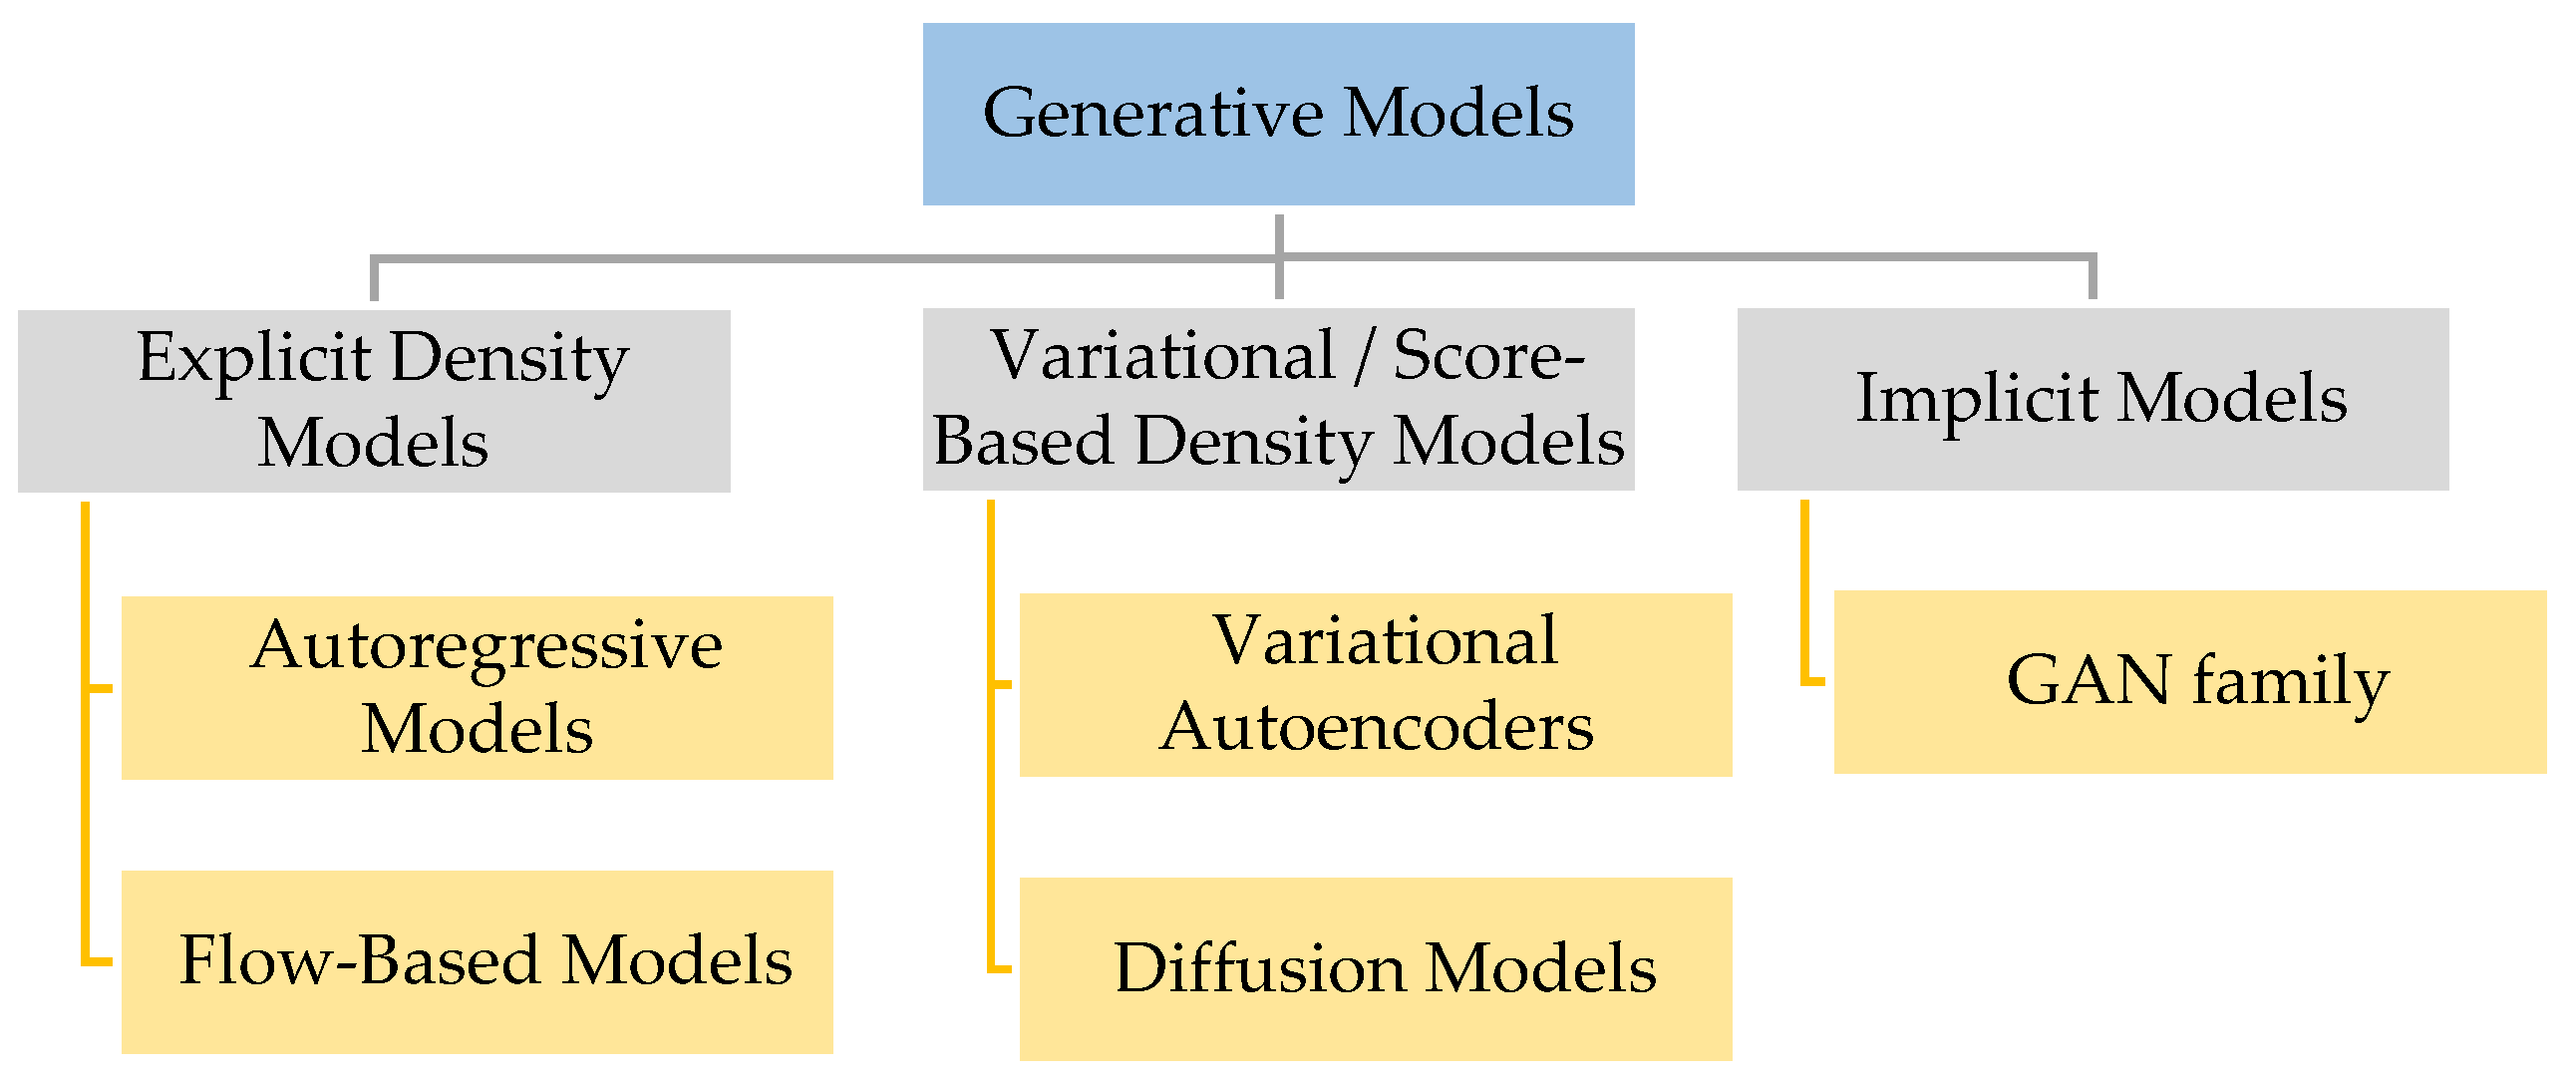
\includegraphics[width=0.92\linewidth]{figures/bcg/gen-models-taxonomy.png}
    \caption{A schematic taxonomy of the principal families of deep generative
    models. Each paradigm differs fundamentally in its training objective,
    inductive biases, and inference procedure.}
    \label{fig:generative_taxonomy}
\end{figure}

Each family embodies a distinct inductive bias and optimization strategy,
yielding characteristic trade-offs between sample quality, training stability,
mode coverage, and inference speed. The remainder of this chapter develops
the mathematical foundations of each paradigm in turn. This sets up the historical foundations before we move on and introduce our methodology in Chapter~\ref{chap:framework}

% -------------------------------------------------------------------

\section{Variational Autoencoders (VAEs)}
\label{sec:vaes}

Variational Autoencoders, introduced concurrently by Kingma and Welling
\cite{kingma2013auto} and Rezende, Mohamed, and Wierstra \cite{rezende2014stochastic},
provided one of the first scalable frameworks for approximate Bayesian inference
in deep latent variable models. The VAE posits a generative process in which
observations $\mathbf{x}$ are produced from latent variables
$\mathbf{z} \in \mathbb{R}^k$ via a learned decoder $p_\theta(\mathbf{x} \mid \mathbf{z})$,
combined with a prior $p(\mathbf{z})$ — typically an isotropic Gaussian
$\mathcal{N}(\mathbf{0}, \mathbf{I})$:

\begin{equation}
    p_\theta(\bm{x}) = \int p_\theta(\bm{x} \mid \bm{z})\, p(\bm{z})\, \mathrm{d}\bm{z}.
    \label{eq:vae_marginal}
\end{equation}

Because the integral in Equation~\ref{eq:vae_marginal} is intractable for
expressive decoders, direct maximum likelihood estimation is infeasible. The
VAE resolves this by introducing an approximate posterior (encoder)
$q_\phi(\mathbf{z} \mid \mathbf{x})$, parameterised by $\phi$, and optimising
the Evidence Lower Bound (ELBO):

\begin{equation}
    \mathcal{L}_{\text{ELBO}}(\theta, \phi;\, \mathbf{x}) =
    \mathbb{E}_{q_\phi(\mathbf{z} \mid \mathbf{x})}
    \bigl[\log p_\theta(\mathbf{x} \mid \mathbf{z})\bigr]
    - D_{\text{KL}}\bigl(q_\phi(\mathbf{z} \mid \mathbf{x}) \,\|\, p(\mathbf{z})\bigr),
    \label{eq:elbo}
\end{equation}

\noindent where $D_{\text{KL}}(\cdot \| \cdot)$ denotes the KL divergence. The
first term in Equation~\ref{eq:elbo} is a reconstruction likelihood that
encourages the decoder to faithfully recover the input, while the second term
acts as a regulariser that prevents the approximate posterior from deviating
arbitrarily from the prior. By jointly optimising $\theta$ and $\phi$ through
the \emph{reparameterisation trick} — which rewrites the expectation as
$\mathbf{z} = \boldsymbol{\mu}_\phi(\mathbf{x}) +
\boldsymbol{\sigma}_\phi(\mathbf{x}) \odot \boldsymbol{\epsilon}$,
$\boldsymbol{\epsilon} \sim \mathcal{N}(\mathbf{0}, \mathbf{I})$ — the ELBO
becomes differentiable with respect to both parameter sets, enabling
end-to-end training via stochastic gradient descent.

The VAE framework offered several decisive advantages over its predecessors.
First, it scales naturally to high-dimensional data through the use of deep
convolutional architectures for both encoder and decoder. Second, the learned
latent space is continuous and structured, facilitating smooth interpolation
between data points — a property with direct utility in representation learning
and data augmentation. Third, the probabilistic
formulation provides a principled mechanism for handling uncertainty.

Nonetheless, VAEs are subject to well-documented limitations. The KL term in
the ELBO encourages the posterior to collapse towards the prior when the
decoder is sufficiently expressive, a phenomenon termed \emph{posterior
collapse}. Furthermore, optimising the ELBO
under a simple Gaussian likelihood tends to produce blurry samples in
pixel space, as the model distributes probability mass broadly to minimise
the expected reconstruction error. Numerous
extensions have been proposed to mitigate these shortcomings, including
hierarchical VAEs and the introduction
of normalising flow posteriors \cite{rezende2015variational}. Nevertheless,
as image generation benchmarks evolved, adversarial and, ultimately, diffusion-based approaches gained more popularity,

% -------------------------------------------------------------------

\section{Generative Adversarial Networks (GANs)}
\label{sec:gans}

Generative Adversarial Networks, proposed by Goodfellow et al.\
\cite{goodfellow2014generative}, reconceived image synthesis as a competitive
game between two neural networks: a \emph{generator} $G_\theta : \mathcal{Z}
\to \mathcal{X}$ that maps samples from a simple latent distribution
$p_\mathbf{z}(\mathbf{z})$ to the data space, and a \emph{discriminator}
$D_\phi : \mathcal{X} \to [0, 1]$ that attempts to distinguish real samples
from generated ones. The original formulation casts this as the following
minimax problem:

\begin{equation}
    \min_\theta \max_\phi \; \mathcal{V}(G_\theta, D_\phi) =
    \mathbb{E}_{\mathbf{x} \sim p_{\text{data}}}[\log D_\phi(\mathbf{x})]
    + \mathbb{E}_{\mathbf{z} \sim p_\mathbf{z}}
    [\log(1 - D_\phi(G_\theta(\mathbf{z})))].
    \label{eq:gan_objective}
\end{equation}

At the theoretical optimum, the discriminator $D_\phi^*(\mathbf{x}) =
p_{\text{data}}(\mathbf{x}) / (p_{\text{data}}(\mathbf{x}) + p_\theta(\mathbf{x}))$
and the generator objective reduces to minimising the Jensen--Shannon divergence
between $p_{\text{data}}$ and $p_\theta$ \cite{goodfellow2014generative}.
Critically, the generator never accesses the training data directly; it
receives gradient information solely through the discriminator, thereby
circumventing the need for an explicit likelihood model. This implicit
generative approach unlocks a substantially richer hypothesis class for the
generator, yielding significantly sharper samples than the VAE under
comparable architectural budgets.

There was a rapid growth in the GAN framework in the years after its initial introduction. The Deep Convolutional GAN (DCGAN)
demonstrated that architectural guidelines — such as the use of strided
convolutions, batch normalisation, and the avoidance of pooling layers — were
essential for stable training. Subsequent theoretical analyses revealed that
the Jensen--Shannon divergence underlying Equation~\ref{eq:gan_objective}
is poorly behaved when the supports of $p_{\text{data}}$ and $p_\theta$ are
disjoint, a condition commonly encountered early in training. The Wasserstein
GAN (WGAN) addressed this by replacing the
JS divergence with the earth mover's distance:

\begin{equation}
    W(p_{\text{data}}, p_\theta) =
    \sup_{\|f\|_L \leq 1} \mathbb{E}_{\mathbf{x} \sim p_{\text{data}}}[f(\mathbf{x})]
    - \mathbb{E}_{\hat{\mathbf{x}} \sim p_\theta}[f(\hat{\mathbf{x}})],
    \label{eq:wasserstein}
\end{equation}

\noindent where the supremum is taken over all 1-Lipschitz functions $f$.
This reformulation yields more meaningful gradients throughout training and
substantially improves stability. The practical enforcement of the Lipschitz
constraint was subsequently refined through gradient penalty regularisation.

Progressive training strategies \cite{karras2018progressive} and large-scale
normalisation techniques further expanded the resolution ceiling of GAN
synthesis. The StyleGAN series demonstrated state-of-the-art perceptual quality on
high-resolution face generation by introducing a style-based generator
architecture that disentangles coarse and fine-grained attributes in the
latent space. Concurrently, large-scale class-conditional models such as
BigGAN pushed the Fréchet Inception Distance (FID)
\cite{heusel2017gans} on ImageNet to levels previously considered
unattainable, establishing GANs as the dominant paradigm for high-fidelity
image synthesis through the late 2010s.

\begin{figure}[ht]
    \centering
    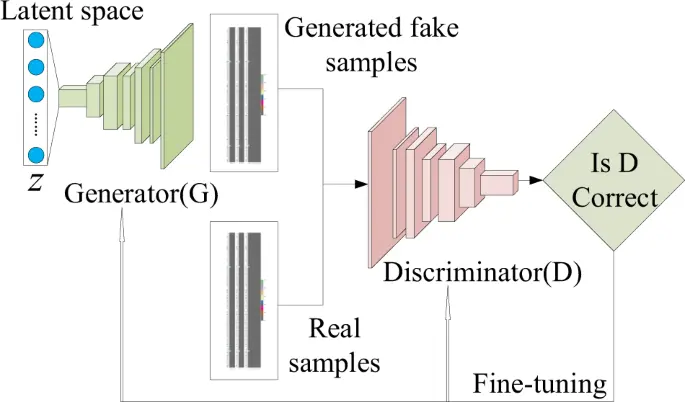
\includegraphics[width=0.85\linewidth]{figures/bcg/GAN.png}
    \caption{Schematic illustration of the GAN training procedure. The generator
    $G_\theta$ maps latent vectors $\mathbf{z}$ to synthetic images, while the
    discriminator $D_\phi$ produces a real/fake classification score.
    Gradients flow from $D_\phi$ back through $G_\theta$, with no direct access
    to the training data.}
    \label{fig:gan_diagram}
\end{figure}

Despite their impressive empirical performance, GANs are afflicted by several
fundamental difficulties. Training instability — characterised by oscillating
losses, gradient vanishing in the discriminator, and sensitivity to
hyperparameter choices — has been widely documented \cite{salimans2016improved}.
Mode collapse, wherein the generator produces samples of high perceptual
quality but low diversity, represents a particularly acute failure mode:
the generator may identify a small subset of the data manifold that reliably
deceives the discriminator and exploit it exclusively, thereby failing to
cover $p_{\text{data}}$ in its entirety . The
adversarial training objective provides no explicit mechanism for diversity
enforcement, and the practical mitigations — minibatch discrimination
\cite{salimans2016improved}, unrolled GANs — offer
only partial remedies. These intrinsic limitations, combined with the
comparatively greater training stability of likelihood-based methods, motivated
renewed interest in alternative generative paradigms, and ultimately contributed
to the ascendance of diffusion-based models as the dominant framework for
high-quality image synthesis \cite{dhariwal2021diffusion}.









































\section{Diffusion and Score-Based Generative Models}
\label{sec:diffusion}

Diffusion-based generative models represent a paradigm shift in the design of
deep generative systems, achieving unprecedented levels of sample fidelity and
diversity on complex image distributions \cite{dhariwal2021diffusion}. In
contrast to GANs, which rely on an adversarial training signal, or VAEs, which
optimise a variational lower bound on the likelihood, diffusion models learn to
reverse a stochastic \emph{noising process} that gradually destroys structure
in the data. The generative procedure is then conceived as the time-reversal
of this destruction: beginning from pure noise, the model iteratively denoises
a latent state until a coherent sample is recovered. This section develops the
mathematical foundations of the three principal formulations of this idea:
Denoising Diffusion Probabilistic Models (DDPMs), score-based generative
modelling via score matching, and the unifying perspective achieved through
stochastic differential equations (SDEs).

% -------------------------------------------------------------------

\subsection{Denoising Diffusion Probabilistic Models}
\label{subsec:ddpm}

Denoising Diffusion Probabilistic Models, introduced by Ho et al.\
\cite{ho2020denoising} and building upon the foundational work of Sohl-Dickstein
et al.\ \cite{sohl2015deep}, define a latent variable model over a sequence of
variables $\mathbf{x}_0, \mathbf{x}_1, \ldots, \mathbf{x}_T$, where
$\mathbf{x}_0 \sim p_{\text{data}}$ denotes a clean data sample and
$\mathbf{x}_T$ is approximately distributed as an isotropic Gaussian
$\mathcal{N}(\mathbf{0}, \mathbf{I})$ for a sufficiently large $T$.

\paragraph{The Forward Process.}
The \emph{forward} (or \emph{diffusion}) process $q$ is a fixed, non-learnable
Markov chain that incrementally corrupts the data by adding small amounts of
Gaussian noise at each step $t \in \{1, \ldots, T\}$:

\begin{equation}
    q(\mathbf{x}_t \mid \mathbf{x}_{t-1}) =
    \mathcal{N}\!\left(\mathbf{x}_t;\;
    \sqrt{1 - \beta_t}\,\mathbf{x}_{t-1},\; \beta_t \mathbf{I}\right),
    \label{eq:ddpm_forward_step}
\end{equation}

\noindent where $\{\beta_t\}_{t=1}^T \subset (0, 1)$ is a fixed variance
schedule, typically chosen to be monotonically increasing. A key analytical
benefit of this Markov structure is that the marginal $q(\mathbf{x}_t
\mid \mathbf{x}_0)$ is available in closed form. Defining
$\alpha_t = 1 - \beta_t$ and $\bar{\alpha}_t = \prod_{s=1}^{t} \alpha_s$,
one obtains:

\begin{equation}
    q(\mathbf{x}_t \mid \mathbf{x}_0) =
    \mathcal{N}\!\left(\mathbf{x}_t;\;
    \sqrt{\bar{\alpha}_t}\,\mathbf{x}_0,\;
    (1 - \bar{\alpha}_t)\mathbf{I}\right),
    \label{eq:ddpm_marginal}
\end{equation}

which allows arbitrary noisy latents to be sampled from $\mathbf{x}_0$
in a single step via the reparameterisation
$\mathbf{x}_t = \sqrt{\bar{\alpha}_t}\,\mathbf{x}_0 +
\sqrt{1 - \bar{\alpha}_t}\,\boldsymbol{\epsilon}$,
$\boldsymbol{\epsilon} \sim \mathcal{N}(\mathbf{0}, \mathbf{I})$.
This property is fundamental to the efficient training procedure described
below.

\paragraph{The Reverse Process.}
The \emph{reverse} (or \emph{generative}) process $p_\theta$ is a learned
Markov chain that operates in the opposite temporal direction, progressively
denoising a sample initialised from $\mathbf{x}_T \sim \mathcal{N}(\mathbf{0},
\mathbf{I})$:

\begin{equation}
    p_\theta(\mathbf{x}_{t-1} \mid \mathbf{x}_t) =
    \mathcal{N}\!\left(\mathbf{x}_{t-1};\;
    \boldsymbol{\mu}_\theta(\mathbf{x}_t, t),\;
    \Sigma_\theta(\mathbf{x}_t, t)\right).
    \label{eq:ddpm_reverse}
\end{equation}

The true reverse posterior $q(\mathbf{x}_{t-1} \mid \mathbf{x}_t, \mathbf{x}_0)$
is tractable and Gaussian when conditioned on $\mathbf{x}_0$:

\begin{equation}
    q(\mathbf{x}_{t-1} \mid \mathbf{x}_t, \mathbf{x}_0) =
    \mathcal{N}\!\left(\mathbf{x}_{t-1};\;
    \tilde{\boldsymbol{\mu}}_t(\mathbf{x}_t, \mathbf{x}_0),\;
    \tilde{\beta}_t \mathbf{I}\right),
    \label{eq:ddpm_posterior}
\end{equation}

\noindent with $\tilde{\boldsymbol{\mu}}_t(\mathbf{x}_t, \mathbf{x}_0) =
\frac{\sqrt{\bar{\alpha}_{t-1}}\beta_t}{1 - \bar{\alpha}_t}\mathbf{x}_0 +
\frac{\sqrt{\alpha_t}(1 - \bar{\alpha}_{t-1})}{1 - \bar{\alpha}_t}\mathbf{x}_t$
and $\tilde{\beta}_t = \frac{1 - \bar{\alpha}_{t-1}}{1 - \bar{\alpha}_t}\beta_t$.

\paragraph{Training Objective.}
Training proceeds by minimising a variational upper bound on the negative
log-likelihood, which decomposes over diffusion steps. Ho et al.\
\cite{ho2020denoising} showed that, after several simplifications, the
dominant contribution reduces to a reweighted denoising objective. In its
most widely adopted form, the model is parameterised as a noise-prediction
network $\boldsymbol{\epsilon}_\theta(\mathbf{x}_t, t)$, and the training
loss is:

\begin{equation}
    \mathcal{L}_{\text{simple}}(\theta) =
    \mathbb{E}_{t,\, \mathbf{x}_0,\, \boldsymbol{\epsilon}}
    \left[\left\|
    \boldsymbol{\epsilon} -
    \boldsymbol{\epsilon}_\theta\!\left(
    \sqrt{\bar{\alpha}_t}\,\mathbf{x}_0 +
    \sqrt{1 - \bar{\alpha}_t}\,\boldsymbol{\epsilon},\; t
    \right)
    \right\|^2\right],
    \label{eq:ddpm_loss}
\end{equation}

\noindent where $t \sim \mathcal{U}\{1, \ldots, T\}$ and
$\boldsymbol{\epsilon} \sim \mathcal{N}(\mathbf{0}, \mathbf{I})$.
This objective is equivalent to denoising score matching at each noise level
\cite{vincent2011connection}, a connection that will be made explicit in the
following subsection. The practical implementation employs a time-conditioned
U-Net architecture \cite{ronneberger2015unet} with sinusoidal timestep
embeddings, a design choice that has since become standard across the field.

Despite achieving sample quality competitive with, and often surpassing, state-of-the-art
GANs on benchmarks such as CIFAR-10 and LSUN \cite{ho2020denoising}, the DDPM
framework incurs a significant computational cost at inference time. Generating
a single sample requires $T$ sequential neural function evaluations — typically
$T = 1000$ — rendering DDPMs substantially slower than single-pass generators
such as GANs. This inference bottleneck is the primary motivation for the
distillation techniques examined in Chapter~\ref{chap:knowledge_distillation}.

% -------------------------------------------------------------------

\subsection{Score-Based Modeling and Score Matching}
\label{subsec:score_matching}

In parallel with the development of DDPMs, Song and Ermon
\cite{song2019generative, song2020improved} developed a distinct but intimately
related framework grounded in the concept of the \emph{score function}.
For a probability distribution $p(\mathbf{x})$, the score function is defined
as the gradient of the log-density with respect to the data:

\begin{equation}
    \mathbf{s}(\mathbf{x}) = \nabla_{\mathbf{x}} \log p(\mathbf{x}).
    \label{eq:score_function}
\end{equation}

The score function encodes the direction of steepest ascent in log-probability
space and is defined without reference to the normalising constant $Z$ in
$p(\mathbf{x}) = \tilde{p}(\mathbf{x}) / Z$. This property is particularly
attractive, as normalising constants are generally intractable for deep energy-based
models. Given access to the score, samples can be generated via
\emph{Langevin dynamics}: starting from an arbitrary initial point
$\mathbf{x}_0$, the chain:

\begin{equation}
    \mathbf{x}_{i+1} = \mathbf{x}_i +
    \frac{\eta}{2}\nabla_{\mathbf{x}} \log p(\mathbf{x}_i) +
    \sqrt{\eta}\,\boldsymbol{\xi}_i, \quad
    \boldsymbol{\xi}_i \sim \mathcal{N}(\mathbf{0}, \mathbf{I}),
    \label{eq:langevin}
\end{equation}

converges in distribution to $p(\mathbf{x})$ as $\eta \to 0$ and the number
of steps tends to infinity. The generative modeling
task then reduces to learning a neural score estimator
$\mathbf{s}_\theta(\mathbf{x}) \approx \nabla_{\mathbf{x}} \log p(\mathbf{x})$.

\paragraph{Score Matching.}
Learning the score directly from data can be achieved through the
\emph{score matching} objective of Hyvärinen \cite{hyvarinen2005estimation}:

\begin{equation}
    \mathcal{J}_{\text{SM}}(\theta) =
    \mathbb{E}_{p(\mathbf{x})}\left[
    \frac{1}{2}\left\|\mathbf{s}_\theta(\mathbf{x})\right\|^2
    + \operatorname{tr}\!\left(\nabla_{\mathbf{x}} \mathbf{s}_\theta(\mathbf{x})\right)
    \right],
    \label{eq:score_matching}
\end{equation}

which avoids the intractable log-likelihood entirely. However, the trace of
the Jacobian in Equation~\ref{eq:score_matching} is computationally expensive
to evaluate for high-dimensional $\mathbf{x}$. \emph{Denoising score matching}
\cite{vincent2011connection} circumvents this by instead training the model
to predict the score of a noise-corrupted data distribution $q_\sigma(\tilde{\mathbf{x}}
\mid \mathbf{x}) = \mathcal{N}(\tilde{\mathbf{x}}; \mathbf{x}, \sigma^2 \mathbf{I})$:

\begin{equation}
    \mathcal{J}_{\text{DSM}}(\theta; \sigma) =
    \mathbb{E}_{\mathbf{x} \sim p_{\text{data}}}\,
    \mathbb{E}_{\tilde{\mathbf{x}} \sim q_\sigma(\cdot|\mathbf{x})}\left[
    \left\|\mathbf{s}_\theta(\tilde{\mathbf{x}}, \sigma) -
    \nabla_{\tilde{\mathbf{x}}} \log q_\sigma(\tilde{\mathbf{x}} \mid \mathbf{x})
    \right\|^2\right],
    \label{eq:denoising_score_matching}
\end{equation}

\noindent where $\nabla_{\tilde{\mathbf{x}}} \log q_\sigma(\tilde{\mathbf{x}} \mid \mathbf{x})
= -(\tilde{\mathbf{x}} - \mathbf{x}) / \sigma^2$. The minimiser of
$\mathcal{J}_{\text{DSM}}$ equals the score of the smoothed distribution,
and a direct algebraic substitution reveals that this is equivalent to
learning a noise predictor up to a constant scaling factor — precisely the
DDPM objective of Equation~\ref{eq:ddpm_loss}. This connection,
established rigorously by Ho et al.\ \cite{ho2020denoising}, demonstrates
that DDPMs and score-based models are, at the level of their training objectives,
equivalent formulations of the same underlying idea.

\paragraph{Noise Conditioning and Multi-Scale Estimation.}
A practical difficulty with score matching at a single noise level $\sigma$ is
that the score function becomes uninformative in low-density regions of
$p_{\text{data}}$, precisely where accurate estimation is most critical for
high-quality generation. Song and Ermon \cite{song2019generative, song2020improved}
addressed this by training a \emph{Noise Conditional Score Network} (NCSN) on a
geometric sequence of noise levels
$\{\sigma_i\}_{i=1}^L$ with $\sigma_1 > \sigma_2 > \cdots > \sigma_L \approx 0$,
and performing annealed Langevin dynamics during inference. At large $\sigma$,
the perturbed distribution covers the ambient space densely, enabling robust
initialisation; at small $\sigma$, the score estimate closely tracks the
original data distribution.

% -------------------------------------------------------------------

\subsection{A Unified Framework via SDEs}
\label{subsec:sde}

Song et al.\ \cite{song2021scorebased} provided a unifying perspective that
subsumes both DDPMs and NCSNs as special cases of a continuous-time framework
defined by stochastic differential equations (SDEs). In this formulation, the
discrete Markov chain of the DDPM is replaced by a continuous stochastic
process $\{\mathbf{x}(t)\}_{t \in [0, T]}$, where $t = 0$ corresponds to
clean data and $t = T$ to a tractable noise distribution. The forward
diffusion process is governed by an Itô SDE of the form:

\begin{equation}
    \mathrm{d}\mathbf{x} = \mathbf{f}(\mathbf{x}, t)\,\mathrm{d}t
    + g(t)\,\mathrm{d}\mathbf{w},
    \label{eq:forward_sde}
\end{equation}

\noindent where $\mathbf{f}(\cdot, t) : \mathbb{R}^d \to \mathbb{R}^d$ is
the \emph{drift} coefficient, $g : \mathbb{R} \to \mathbb{R}$ is the scalar
\emph{diffusion} coefficient, and $\mathbf{w}$ is a standard Wiener process
(Brownian motion). The transition kernel $p_{0t}(\mathbf{x}(t) \mid \mathbf{x}(0))$
is Gaussian for the affine drift functions used in practice, and the marginal
distributions $\{p_t\}_{t \in [0,T]}$ evolve from $p_0 = p_{\text{data}}$
towards a tractable prior $p_T \approx \mathcal{N}(\mathbf{0}, \sigma^2_{\max}\mathbf{I})$.

\paragraph{The Reverse-Time SDE.}
Anderson \cite{anderson1982reverse} showed that the time-reversal of a
diffusion process described by Equation~\ref{eq:forward_sde} is itself
an Itô SDE:

\begin{equation}
    \mathrm{d}\mathbf{x} = \left[
    \mathbf{f}(\mathbf{x}, t) -
    g(t)^2 \nabla_{\mathbf{x}} \log p_t(\mathbf{x})
    \right]\mathrm{d}t
    + g(t)\,\mathrm{d}\bar{\mathbf{w}},
    \label{eq:reverse_sde}
\end{equation}

\noindent where $\bar{\mathbf{w}}$ is a Wiener process running in reverse
time, and $\mathrm{d}t$ denotes an infinitesimal negative time increment.
The term $\nabla_{\mathbf{x}} \log p_t(\mathbf{x})$ is the \emph{time-dependent
score function} of the marginal distribution at time $t$. Crucially, if this
score function is known, the reverse SDE is fully specified and can be
integrated numerically to yield samples from $p_0$. The generative modelling
task therefore reduces to learning a time-indexed score network
$\mathbf{s}_\theta(\mathbf{x}, t) \approx \nabla_{\mathbf{x}} \log p_t(\mathbf{x})$,
trained via the continuous-time analogue of the denoising score matching
objective:

\begin{equation}
    \mathcal{L}_{\text{score}}(\theta) =
    \mathbb{E}_{t}\!\left\{
    \lambda(t)\,\mathbb{E}_{\mathbf{x}(0), \mathbf{x}(t)}\!\left[
    \left\|\mathbf{s}_\theta(\mathbf{x}(t), t) -
    \nabla_{\mathbf{x}(t)} \log p_{0t}(\mathbf{x}(t) \mid \mathbf{x}(0))
    \right\|^2\right]\right\},
    \label{eq:score_sde_loss}
\end{equation}

\noindent where $\lambda(t) > 0$ is a weighting function and the expectation
over $t$ is taken uniformly over $[0, T]$.

\paragraph{Special Cases and the Probability Flow ODE.}
The DDPM corresponds to the \emph{Variance Preserving} (VP) SDE, with drift
$\mathbf{f}(\mathbf{x}, t) = -\frac{1}{2}\beta(t)\mathbf{x}$ and diffusion
coefficient $g(t) = \sqrt{\beta(t)}$, where $\beta(t)$ is the continuous-time
analogue of the noise schedule. The NCSN framework of Song and Ermon corresponds
to the \emph{Variance Exploding} (VE) SDE, characterised by zero drift and
$g(t) = \sqrt{\mathrm{d}[\sigma^2(t)]/\mathrm{d}t}$. Both are unified within
the SDE framework of Equation~\ref{eq:forward_sde}--\ref{eq:reverse_sde}.

A particularly consequential consequence of the SDE perspective is the existence
of an associated \emph{probability flow ordinary differential equation} (ODE)
\cite{song2021scorebased}:

\begin{equation}
    \frac{\mathrm{d}\mathbf{x}}{\mathrm{d}t} =
    \mathbf{f}(\mathbf{x}, t) -
    \frac{1}{2}g(t)^2\,\nabla_{\mathbf{x}} \log p_t(\mathbf{x}),
    \label{eq:probability_flow_ode}
\end{equation}

which is a deterministic process sharing the same marginal distributions
$\{p_t\}$ as the reverse SDE. Integrating Equation~\ref{eq:probability_flow_ode}
with an off-the-shelf ODE solver, using $\mathbf{s}_\theta$ in place of the
true score, produces high-quality samples while enabling exact likelihood
computation via the \emph{instantaneous change of variables formula}
\cite{chen2018neural}. Moreover, the probability flow ODE provides the
theoretical basis for accelerated sampling: since the stochastic component
has been eliminated, higher-order deterministic solvers can traverse the
trajectory in far fewer function evaluations than stochastic samplers
\cite{song2021denoising, lu2022dpm}. This observation underpins a
broad family of inference-time acceleration methods, including DDIM
\cite{song2021denoising} and DPM-Solver \cite{lu2022dpm}, which
reduce the number of required neural function evaluations by one to two
orders of magnitude relative to naive ancestral sampling, and constitute
the immediate precursors to the knowledge distillation approaches examined
in Chapter~\ref{chap:knowledge_distillation}.

\begin{figure}[ht]
    \centering
    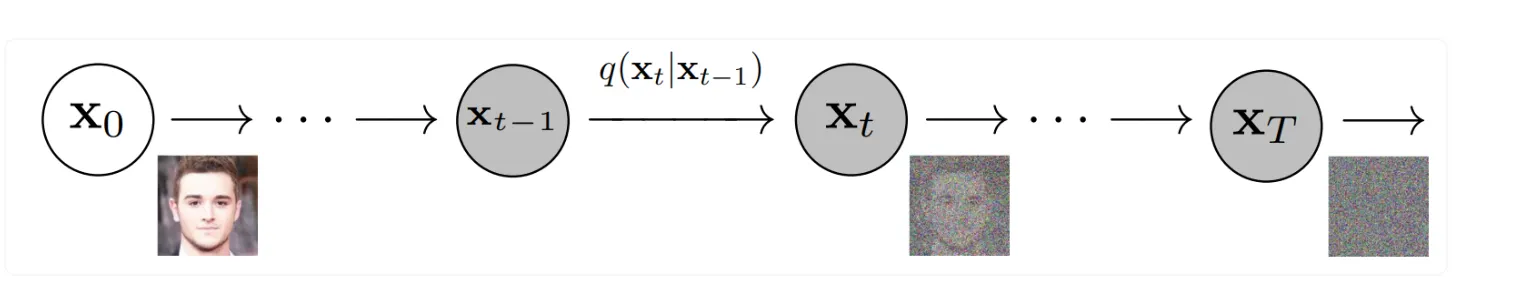
\includegraphics[width=0.95\linewidth]{figures/bcg/SFE-F-B.png}
    \caption{Illustration of the forward adiffusion processes in
    the SDE framework. The forward SDE (top) gradually corrupts data
    $\mathbf{x}(0) \sim p_{\text{data}}$ into noise $\mathbf{x}(T) \sim p_T$
    over continuous time}
    \label{fig:sde_forward_reverse}
\end{figure}

The SDE framework thus provides three practically significant contributions.
First, it provides a rigorous theoretical framework — grounded in stochastic
calculus — that bridges the relationship between previously distinct modeling concepts. Second, it decouples the \emph{design} of the forward process
(the choice of SDE) from the \emph{training} of the reverse model (score
matching), permitting principled exploration of novel noise schedules and
process geometries. Third, and most directly relevant to the present work,
the probability flow ODE reveals that the generative process of a diffusion
model can be expressed as a continuous trajectory in data space.


% =============================================================
\section{Flow Matching}
\label{sec:flow_matching}
% =============================================================

Diffusion models and score-based generative models, as discussed in the preceding sections,
construct a stochastic transport between a data distribution $p_{\text{data}}$ and a tractable
noise distribution through a \emph{fixed}, physically motivated degradation process. While
powerful, this design choice imposes constraints on training and inference efficiency:
the reverse process must be simulated over many discrete time steps, and the forward
noising schedule is not optimized for the geometry of the data. Flow matching constitutes
a complementary paradigm that frames generative modeling as the problem of learning a
\emph{deterministic} vector field whose associated ordinary differential equation (ODE)
transports samples from a source distribution to a target distribution in a principled,
simulation-free manner \cite{lipman2022flow, liu2022flow, albergo2023building}.
This section develops the theoretical foundations of flow matching, beginning with the
continuous normalizing flow framework, proceeding to the flow matching objective and
its conditional formulation, and concluding with the role of optimal transport and
rectified flows in producing straight, efficient trajectories.

% -------------------------------------------------------------
\subsection{Continuous Normalizing Flows}
\label{subsec:cnf}
% -------------------------------------------------------------

Normalizing flows define a family of generative models that express the data distribution
$p_1$ as an exact change-of-variables transformation of a simple base distribution
$p_0 = \mathcal{N}(\mathbf{0}, \mathbf{I})$. In discrete normalizing flows
\cite{rezende2015variational, dinh2016density}, this transformation is composed of a finite
sequence of invertible, differentiable mappings with analytically tractable Jacobian
determinants. Continuous normalizing flows (CNFs) \cite{chen2018neural} generalize this
construction by parameterizing the transformation as the solution to an autonomous
ordinary differential equation:

\begin{equation}
    \frac{d\mathbf{x}(t)}{dt} = v_\theta(\mathbf{x}(t),\, t), \quad t \in [0, 1],
    \label{eq:cnf_ode}
\end{equation}

\noindent where $\mathbf{x}(t) \in \mathbb{R}^d$ is the state of the system at time $t$,
and $v_\theta : \mathbb{R}^d \times [0,1] \to \mathbb{R}^d$ is a time-dependent vector
field parameterized by a neural network with parameters $\theta$. Given an initial
condition $\mathbf{x}(0) \sim p_0$, integrating the ODE in Equation~\ref{eq:cnf_ode}
forward in time from $t=0$ to $t=1$ yields a sample $\mathbf{x}(1) \sim p_1$, defining
the push-forward $p_1 = [\phi_1]_\# p_0$ where $\phi_t$ denotes the \emph{flow map}
associated with $v_\theta$.

The instantaneous change in log-density along a trajectory is governed by the
instantaneous change-of-variables formula \cite{chen2018neural}:

\begin{equation}
    \frac{d \log p_t(\mathbf{x}(t))}{dt} = -\nabla_{\mathbf{x}} \cdot v_\theta(\mathbf{x}(t), t),
    \label{eq:cnf_density}
\end{equation}

\noindent where $\nabla_{\mathbf{x}} \cdot v_\theta$ denotes the divergence of the
vector field. Equation~\ref{eq:cnf_density} enables exact likelihood computation by
integrating both the state and the log-density jointly; however, computing the
divergence in full generality requires $\mathcal{O}(d^2)$ operations or the use of
the Hutchinson stochastic trace estimator \cite{hutchinson1989stochastic}, which introduces
variance into training. Furthermore, CNF training requires solving an ODE at every
gradient step, rendering naive maximum-likelihood training computationally prohibitive
at scale. Flow matching addresses both of these limitations.

% -------------------------------------------------------------
\subsection{The Flow Matching Objective}
\label{subsec:flow_matching_objective}
% -------------------------------------------------------------

The central insight of flow matching \cite{lipman2022flow} is that one can train a CNF
without ever simulating the ODE during training, provided that a \emph{target} vector
field whose flow interpolates between $p_0$ and $p_1$ can be specified. Let
$p_t : [0,1] \to \mathcal{P}(\mathbb{R}^d)$ be a time-indexed probability path such
that $p_0 = \mathcal{N}(\mathbf{0}, \mathbf{I})$ and $p_1 \approx p_{\text{data}}$.
A vector field $u_t(\mathbf{x})$ is said to \emph{generate} the path $p_t$ if the
associated continuity equation is satisfied:

\begin{equation}
    \frac{\partial p_t(\mathbf{x})}{\partial t} + \nabla_{\mathbf{x}} \cdot \bigl(p_t(\mathbf{x})\, u_t(\mathbf{x})\bigr) = 0.
    \label{eq:continuity}
\end{equation}

The marginal flow matching (MFM) objective regresses the neural vector field $v_\theta$
directly onto $u_t$:

\begin{equation}
    \mathcal{L}_{\text{FM}}(\theta) = \mathbb{E}_{t \sim \mathcal{U}[0,1],\, \mathbf{x} \sim p_t}
    \bigl\| v_\theta(\mathbf{x}, t) - u_t(\mathbf{x}) \bigr\|^2.
    \label{eq:fm_loss}
\end{equation}

Although this objective is well-posed in principle, the marginal vector field $u_t(\mathbf{x})$
is generally intractable because it requires integrating over all data points that
could have generated a given noisy sample $\mathbf{x}$ at time $t$. Lipman et al.\
\cite{lipman2022flow} resolve this through the \emph{conditional flow matching} (CFM)
formulation. For each data sample $\mathbf{x}_1 \sim p_{\text{data}}$, one defines a
\emph{conditional} probability path $p_t(\mathbf{x} \mid \mathbf{x}_1)$ and an
associated conditional vector field $u_t(\mathbf{x} \mid \mathbf{x}_1)$, chosen such
that the marginals $p_t(\mathbf{x}) = \int p_t(\mathbf{x} \mid \mathbf{x}_1)\,
p_{\text{data}}(\mathbf{x}_1)\, d\mathbf{x}_1$ recover the desired path. The
conditional flow matching loss is then:

\begin{equation}
    \mathcal{L}_{\text{CFM}}(\theta) = \mathbb{E}_{t,\, \mathbf{x}_1 \sim p_{\text{data}},\,
    \mathbf{x} \sim p_t(\cdot \mid \mathbf{x}_1)}
    \bigl\| v_\theta(\mathbf{x}, t) - u_t(\mathbf{x} \mid \mathbf{x}_1) \bigr\|^2.
    \label{eq:cfm_loss}
\end{equation}

A key theoretical result establishes that $\mathcal{L}_{\text{CFM}}$ and
$\mathcal{L}_{\text{FM}}$ share identical gradients with respect to $\theta$
\cite{lipman2022flow}, meaning the conditional objective can be minimized in place of
the intractable marginal objective without any approximation. A natural and widely
adopted choice for the conditional path is the Gaussian interpolant:

\begin{align}
    p_t(\mathbf{x} \mid \mathbf{x}_1) &= \mathcal{N}\!\left(\mathbf{x};\; \mu_t(\mathbf{x}_1),\; \sigma_t^2 \mathbf{I}\right), \label{eq:gaussian_path}\\
    \mu_t(\mathbf{x}_1) &= \bigl(1 - (1 - \sigma_{\min})t\bigr)\,\mathbf{x}_0 + t\,\mathbf{x}_1, \label{eq:interpolant_mean}
\end{align}

\noindent with $\sigma_{\min} \ll 1$ controlling residual noise at $t=1$. The
corresponding conditional vector field admits the closed form:

\begin{equation}
    u_t(\mathbf{x} \mid \mathbf{x}_1) = \frac{\mathbf{x}_1 - (1 - \sigma_{\min})\mathbf{x}_0}
    {1 - (1 - \sigma_{\min})t},
    \label{eq:conditional_vf}
\end{equation}

\noindent which is a \emph{constant} vector field pointing from $\mathbf{x}_0$ to
$\mathbf{x}_1$ along a straight line. This observation has profound implications for
inference efficiency: if $v_\theta$ learns to reproduce straight-line trajectories, a
single Euler integration step suffices for generation, a property exploited directly
by consistency models \cite{song2023consistency} and rectified flows \cite{liu2022flow},
as discussed in Chapter~\ref{chap:knowledge_distillation}.

\begin{figure}[ht]
    \centering
    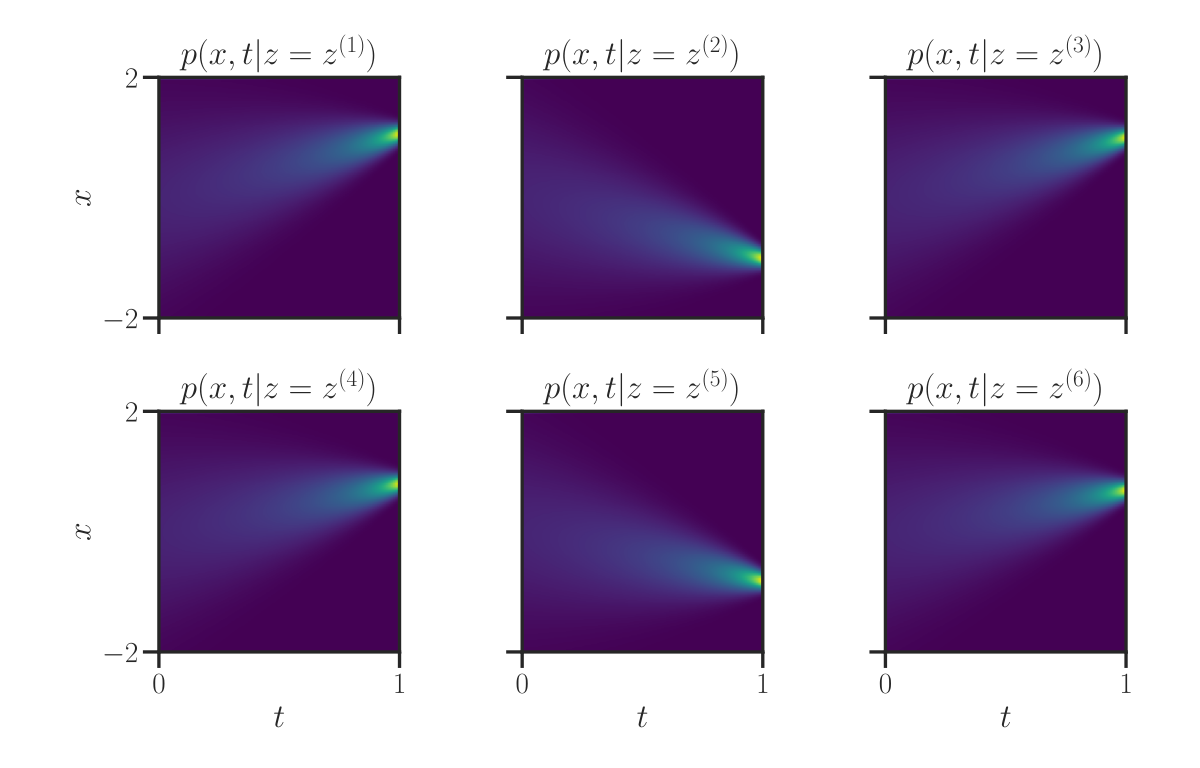
\includegraphics[width=0.85\linewidth]{figures/bcg/FM-CFM.png}
    \caption{Conditional probability paths as linear interpolation. $p(x|t, z = z^{(i)})$ for six samples $z^{(i)}$ (each being a pair $(x_0, x_1)$)}
    \label{fig:cfm_trajectories}
\end{figure}

% -------------------------------------------------------------
\subsection{Optimal Transport and Rectified Flows}
\label{subsec:ot_rectified}
% -------------------------------------------------------------

The freedom to specify the coupling between $p_0$ and $p_1$ in the CFM framework gives
rise to a natural optimization question: which coupling minimizes the average trajectory
length, and thus minimizes the integration error incurred during inference with a
finite-step ODE solver? This question is answered by the theory of optimal transport (OT)
\cite{villani2009optimal}.

Formally, given two distributions $p_0$ and $p_1$ on $\mathbb{R}^d$, the
$\ell^2$-optimal transport plan $\pi^* \in \mathcal{P}(\mathbb{R}^d \times \mathbb{R}^d)$
solves the Monge--Kantorovich problem:

\begin{equation}
    \pi^* = \underset{\pi \in \Pi(p_0,\, p_1)}{\arg\min}\;
    \mathbb{E}_{(\mathbf{x}_0, \mathbf{x}_1) \sim \pi}
    \bigl[\|\mathbf{x}_1 - \mathbf{x}_0\|^2\bigr],
    \label{eq:ot_problem}
\end{equation}

\noindent where $\Pi(p_0, p_1)$ denotes the set of all joint distributions with
marginals $p_0$ and $p_1$. $\pi^*$ is induced by a deterministic map $T^*$, i.e.\
$\pi^* = (\text{Id} \times T^*)_\# p_0$, and the optimal trajectories are straight
lines. Lipman et al.\ \cite{lipman2022flow} refer to the CFM variant that employs the
OT plan as \emph{OT-CFM}, and demonstrate empirically that it produces significantly
straighter flows and requires fewer function evaluations at inference time compared to
the independent coupling $\pi_{\text{ind}} = p_0 \otimes p_1$.

An independent but closely related approach, \emph{Rectified Flow} (RF) \cite{liu2022flow},
addresses the same problem of flow straightening through an iterative reflow procedure.
The core observation is that the linear interpolant between independently sampled pairs
$(\mathbf{x}_0, \mathbf{x}_1)$ defines a valid training target but may produce
trajectories that cross one another in data space, resulting in a non-straight marginal
vector field. Rectified flow proceeds as follows: given a coupling $\pi^{(k)}$ at
iteration $k$, one trains a vector field $v_\theta^{(k)}$ with the CFM loss under
$\pi^{(k)}$, generates paired samples $(\mathbf{x}_0, \hat{\mathbf{x}}_1)$ by
simulating $v_\theta^{(k)}$, and defines the refined coupling
$\pi^{(k+1)} = \text{Law}(\mathbf{x}_0, \hat{\mathbf{x}}_1)$. This reflow operation
progressively straightens trajectories, as proved in \cite{liu2022flow} through the
monotone decrease of the expected squared trajectory curvature.

The stochastic interpolants framework of Albergo and Vanden-Eijnden
\cite{albergo2023building} provides a unifying perspective that subsumes both flow
matching and score-based diffusion models. In that framework, an interpolant
$\mathbf{x}(t) = \alpha_t \mathbf{x}_1 + \beta_t \mathbf{x}_0 + \gamma_t \boldsymbol{\epsilon}$
with $\boldsymbol{\epsilon} \sim \mathcal{N}(\mathbf{0}, \mathbf{I})$ induces a
probability path whose generating vector field can be expressed either as a drift
(yielding an ODE) or as a drift-diffusion pair (yielding an SDE), depending on whether
$\gamma_t$ is identically zero. When $\gamma_t = 0$ and the coupling is the OT plan,
one recovers a deterministic OT-CFM; when $\gamma_t > 0$, the framework recovers
the DDPM forward process as a special case \cite{ho2020denoising}. This unification
demonstrates that diffusion models and flow-based models differ not in kind but in the
choice of trajectory geometry and stochasticity, a distinction with direct consequences
for the design of knowledge distillation strategies.

\begin{figure}[ht]
    \centering
    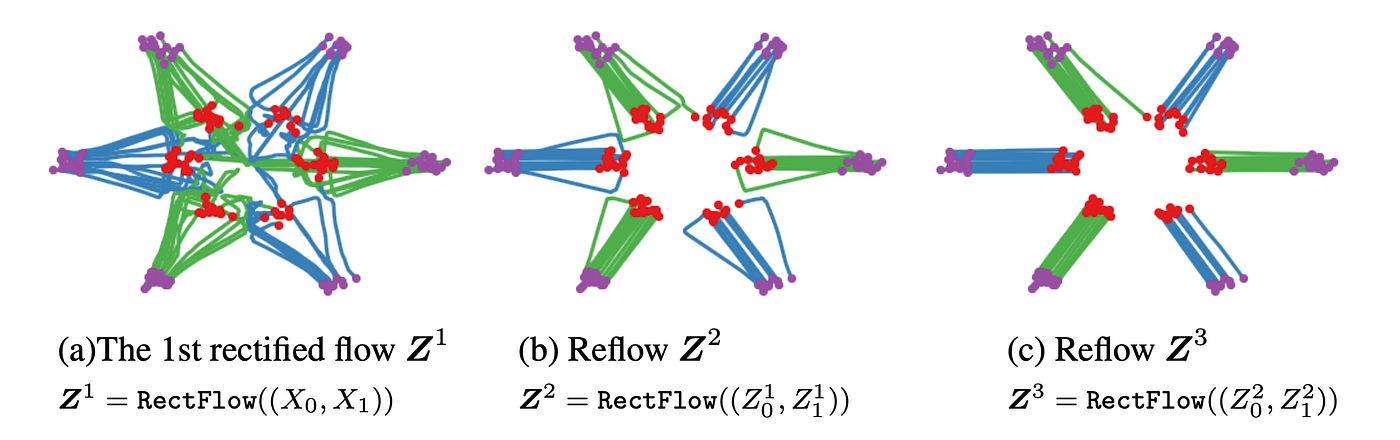
\includegraphics[width=0.82\linewidth]{figures/bcg/RF.png}
    \caption{Schematic of the rectified flow reflow procedure. a): an initial
    1-Rectified Flow trained on independent couplings exhibits crossing trajectories.
    b): after a single reflow step (2-Rectified Flow), trajectories become
    approximately straight. c): 3-Rectified Flow trajectories have become completely straight.}
    \label{fig:rectified_flow}
\end{figure}

In summary, flow matching provides a simulation-free, likelihood-free training framework
for continuous normalizing flows whose flexibility in specifying the probability path
and source-target coupling makes it highly desirable formulation in modern generative models architecture like the "Just Image Transformer" that we will see in Chapter~\ref{chap:architectures}.
    % ============================================================
\chapter{Image Generation Architectures: From Convolutions to Transformers}
\label{chap:architectures}
% ============================================================

The architectural substrate of a generative model is not merely an implementation detail; it determines the inductive biases brought to bear on the data distribution, the computational complexity of training and inference, and ultimately the fidelity and diversity of the generated outputs. The rapid progress of image generation over the past decade is inseparable from a corresponding evolution in backbone architectures — from the early adoption of convolutional neural networks (CNNs) in adversarial and variational frameworks, through the emergence of U-shaped encoder-decoder networks as the workhorse of score-based and diffusion models, to the more recent integration of the self-attention mechanism and its descendant, the Vision Transformer. This chapter surveys these architectural developments with emphasis on the components most directly relevant to diffusion-based image synthesis and the knowledge distillation paradigms discussed in Chapter~\ref{chap:knowledge_distillation}.

% ============================================================
\section{Convolutional Neural Networks}
\label{sec:cnns}
% ============================================================

Convolutional neural networks, whose modern form was systematized by \cite{lecun1998gradient} and subsequently scaled to deep configurations by \cite{krizhevsky2012imagenet}, established the dominant representational paradigm for visual data throughout the 2010s. Their defining structural property is the exploitation of spatial locality and translational equivariance: a learnable filter $\mathbf{w} \in \mathbb{R}^{k \times k \times C_{\text{in}}}$ is convolved with a feature map $\mathbf{x} \in \mathbb{R}^{H \times W \times C_{\text{in}}}$ to produce an output feature map $\mathbf{y} \in \mathbb{R}^{H' \times W' \times C_{\text{out}}}$, where the same filter weights are shared across all spatial positions. Formally, the output at spatial location $(i, j)$ and output channel $c$ is

\begin{equation}
    \mathbf{y}_{i,j,c} = \sum_{c'=1}^{C_{\text{in}}} \sum_{p=0}^{k-1} \sum_{q=0}^{k-1} \mathbf{w}_{p,q,c',c} \cdot \mathbf{x}_{s \cdot i + p,\; s \cdot j + q,\; c'},
    \label{eq:convolution}
\end{equation}

where $s$ denotes the stride. This parameter-sharing scheme yields a substantially smaller model compared to a fully connected layer operating on the same input dimensions, and simultaneously encodes the prior that meaningful visual patterns can occur at arbitrary spatial locations.

Progressive downsampling via strided convolutions or pooling operations reduces the spatial resolution while increasing the number of feature channels, enabling a hierarchical extraction of features at multiple scales. Early layers respond to low-level statistics such as edges and color gradients; deeper layers encode increasingly abstract, semantically meaningful representations \cite{zeiler2014visualizing}. This multi-scale hierarchy is a property that generative architectures have deliberately preserved and exploited.

Normalization layers, principally Batch Normalization \cite{ioffe2015batch} and, later, Group Normalization \cite{wu2018group}, proved essential for stabilizing the training of deep convolutional stacks by reducing internal covariate shift. In the context of generative models conditioned on auxiliary information — such as the diffusion timestep $t$ or a class label — adaptive normalization schemes, specifically Adaptive Group Normalization and Adaptive Layer Normalization, were introduced to modulate intermediate feature representations \cite{dhariwal2021diffusion}. In these schemes, the affine parameters $(\gamma, \beta)$ of the normalization are not fixed scalars but are instead predicted from a conditioning embedding, allowing the network to adjust its internal feature statistics as a function of the condition.

% ============================================================
\subsection{U-Net and its Role in Diffusion}
\label{subsec:unet}
% ============================================================

The U-Net architecture, introduced by \cite{ronneberger2015unet} for biomedical image segmentation, represents a pivotal design pattern for tasks that require both global contextual understanding and fine-grained spatial precision. Its defining characteristic is a symmetric encoder-decoder structure augmented with skip connections that bypass the bottleneck and concatenate encoder feature maps directly to their spatially corresponding decoder feature maps.

Formally, denote the encoder as a sequence of resolution-halving blocks $\{E_\ell\}_{\ell=1}^{L}$ and the decoder as a sequence of resolution-doubling blocks $\{D_\ell\}_{\ell=1}^{L}$. The skip connection at level $\ell$ concatenates the encoder output $\mathbf{h}^{E}_\ell$ with the upsampled decoder feature $\mathbf{h}^{D}_{\ell+1}$ prior to processing by $D_\ell$:

\begin{equation}
    \mathbf{h}^{D}_{\ell} = D_\ell\!\left(\left[\mathbf{h}^{D}_{\ell+1};\; \mathbf{h}^{E}_\ell\right]\right),
    \label{eq:unet_skip}
\end{equation}

where $[\cdot\,;\,\cdot]$ denotes channel-wise concatenation. This mechanism preserves high-frequency spatial detail that would otherwise be irrecoverably lost through successive downsampling operations, enabling precise, pixel-level outputs.

The U-Net was adopted as the denoising backbone in the seminal Denoising Diffusion Probabilistic Models (DDPMs) framework of \cite{ho2020denoising}, and it has since become the near-universal architectural choice for diffusion-based image generators \cite{nichol2021improved, dhariwal2021diffusion, rombach2022latent}. Its suitability for this role stems from several complementary properties. First, the denoising task is itself a dense prediction problem: the network must predict the noise $\boldsymbol{\epsilon}$ (or, equivalently, the score $\nabla_{\mathbf{x}_t} \log p(\mathbf{x}_t)$) at every pixel of an input noisy image $\mathbf{x}_t$, which demands that spatial resolution be maintained end-to-end — precisely the function of the decoder and skip connections. Second, the multi-scale feature hierarchy naturally accommodates the multi-frequency nature of image content: low-frequency structure (overall layout, global semantics) is captured at the bottleneck, while high-frequency detail (texture, edges) is routed through the skip connections. Third, the bottleneck of the U-Net serves as a natural site for injecting conditioning information, whether temporal (the diffusion timestep $t$), semantic (a text embedding from a language model), or structural.

\begin{figure}[ht]
    \centering
    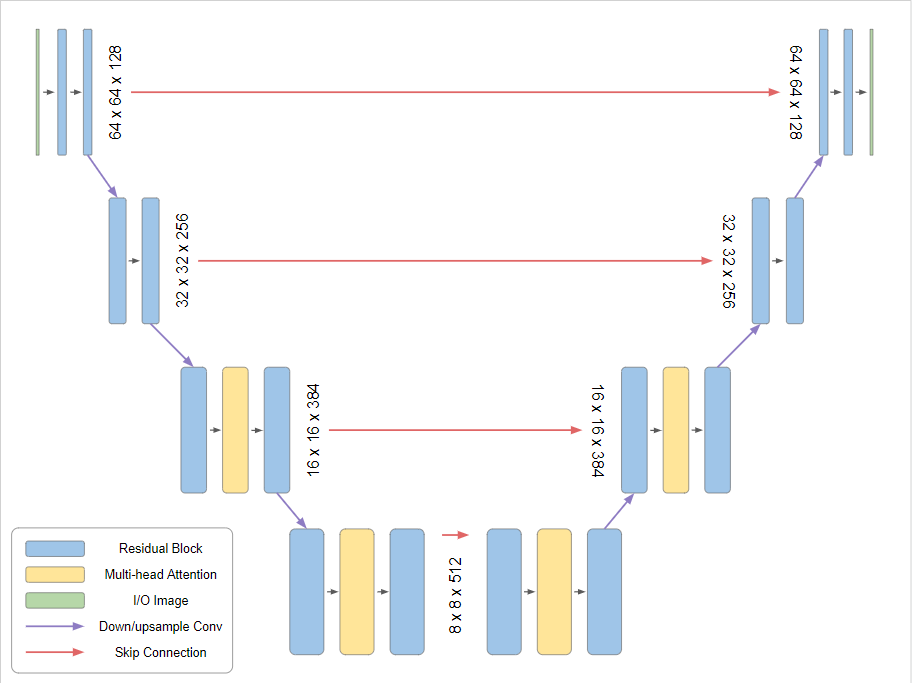
\includegraphics[width=0.85\linewidth]{figures/bcg/unetdiffusion.png}
    \caption{Schematic of a U-Net denoising backbone as employed in diffusion models. Encoder blocks (left) progressively reduce spatial resolution while expanding the channel dimension; decoder blocks (right) reverse this process. Skip connections (horizontal arrows) concatenate encoder features into the corresponding decoder stage. The timestep embedding $\tau(t)$, derived from a sinusoidal encoding, is injected via adaptive normalization at each resolution level.}
    \label{fig:unet_diffusion}
\end{figure}

The specific instantiation of the U-Net used in \cite{dhariwal2021diffusion} — which established a new state of the art for class-conditional image synthesis and whose architecture underpins much of the subsequent work on distillation — departs from the original segmentation-oriented design in several important respects. Each resolution level consists of multiple residual blocks \cite{he2016deep} rather than single convolutional layers, providing increased representational capacity at each scale without altering the spatial resolution. Self-attention layers (discussed in Section~\ref{sec:attention}) are interleaved with the convolutional residual blocks, initially only at the lowest-resolution levels where the global receptive field of attention is computationally tractable, but extending to higher resolutions in the largest model variants. Timestep conditioning is implemented by computing a sinusoidal positional embedding of $t$, projecting it through a small feed-forward network, and using the result to modulate the affine parameters of Group Normalization layers via Adaptive Group Normalization. This architecture served as the direct predecessor to the latent diffusion model U-Nets \cite{rombach2022latent}, and variants of it are employed in many of the knowledge distillation frameworks surveyed in Chapter~\ref{chap:knowledge_distillation}.

% ============================================================
\section{The Attention Mechanism}
\label{sec:attention}
% ============================================================

The attention mechanism, first introduced in the context of sequence-to-sequence neural machine translation by \cite{bahdanau2015neural} and subsequently generalized into the Transformer architecture by \cite{vaswani2017attention}, represents a fundamentally different computational primitive from convolution. Whereas a convolutional filter aggregates information within a fixed local neighborhood, an attention layer computes a weighted aggregation over all positions in a feature map, with the weights themselves being input-dependent. This endows attention-based models with a global receptive field at every layer and the capacity to model long-range dependencies that require many stacked convolutional layers to capture, if they are captured at all.

% ============================================================
\subsection{Self-Attention}
\label{subsec:self_attention}
% ============================================================

In the self-attention formulation, a single input sequence $\mathbf{X} \in \mathbb{R}^{N \times d}$, consisting of $N$ tokens each of dimension $d$, is linearly projected into three distinct representations: the query matrix $\mathbf{Q} = \mathbf{X}\mathbf{W}^Q$, the key matrix $\mathbf{K} = \mathbf{X}\mathbf{W}^K$, and the value matrix $\mathbf{V} = \mathbf{X}\mathbf{W}^V$, where $\mathbf{W}^Q, \mathbf{W}^K, \mathbf{W}^V \in \mathbb{R}^{d \times d_k}$ are learned projection matrices. The attention output is then computed as

\begin{equation}
    \text{Attention}(\mathbf{Q}, \mathbf{K}, \mathbf{V}) = \text{softmax}\!\left(\frac{\mathbf{Q}\mathbf{K}^\top}{\sqrt{d_k}}\right)\mathbf{V},
    \label{eq:self_attention}
\end{equation}

where the factor $\sqrt{d_k}$ is a scaling constant introduced to prevent the dot products from growing too large in magnitude and saturating the softmax function \cite{vaswani2017attention}. The $(i, j)$-th entry of the pre-softmax matrix $\mathbf{Q}\mathbf{K}^\top / \sqrt{d_k}$ can be interpreted as an unnormalized compatibility score between position $i$ and position $j$. After row-wise softmax normalization, these scores form a probability distribution over positions, and the output at position $i$ is a convex combination of all value vectors, weighted by the compatibility of position $i$ with every other position. The computational complexity of this operation is $\mathcal{O}(N^2 d_k)$, which is the primary practical limitation of self-attention when applied to high-resolution images.

When self-attention is applied to two-dimensional feature maps $\mathbf{F} \in \mathbb{R}^{H \times W \times C}$, the spatial dimensions are first flattened into a sequence of $N = H \times W$ tokens, each of dimension $C$. The attention computation then proceeds as described above, after which the output is reshaped back to $\mathbb{R}^{H \times W \times C}$. The quadratic cost in $N$ explains why, in the U-Nets used for diffusion, full self-attention is typically applied only at the lowest-resolution feature maps (e.g., $8 \times 8$ or $16 \times 16$), where $N$ is small, while higher-resolution stages rely on convolutional blocks. Efficient variants such as linear attention \cite{katharopoulos2020transformers} and window-based local attention \cite{liu2021swin} have been proposed to mitigate this bottleneck, and several of these are employed in more recent diffusion architectures.

% ============================================================
\subsection{Multi-Head and Cross-Attention}
\label{subsec:multihead_cross_attention}
% ============================================================

A single attention head, as defined in Equation~\ref{eq:self_attention}, is constrained to learn a single query-key compatibility function operating in a $d_k$-dimensional subspace. Multi-head attention \cite{vaswani2017attention} overcomes this limitation by executing $H$ independent attention computations in parallel, each in a lower-dimensional subspace of dimension $d_k = d / H$, and concatenating their outputs before a final linear projection:

\begin{equation}
    \text{MultiHead}(\mathbf{Q}, \mathbf{K}, \mathbf{V}) = \left[\text{head}_1; \cdots; \text{head}_H\right]\mathbf{W}^O,
    \label{eq:multihead}
\end{equation}

where $\text{head}_h = \text{Attention}(\mathbf{X}\mathbf{W}^Q_h, \mathbf{X}\mathbf{W}^K_h, \mathbf{X}\mathbf{W}^V_h)$ and $\mathbf{W}^O \in \mathbb{R}^{d \times d}$ is the output projection. Empirically, different attention heads specialize in capturing different relational patterns — some may attend to syntactically proximate tokens, others to semantically related but spatially distant regions — and their combination yields richer representations than any single head \cite{voita2019analyzing}.

Cross-attention generalizes the self-attention mechanism to settings in which the queries are derived from one sequence and the keys and values from a distinct, conditioning sequence. Given a primary feature map $\mathbf{Z} \in \mathbb{R}^{N \times d}$ and a conditioning context $\mathbf{C} \in \mathbb{R}^{M \times d_c}$, the cross-attention output is

\begin{equation}
    \text{CrossAttention}(\mathbf{Z}, \mathbf{C}) = \text{softmax}\!\left(\frac{(\mathbf{Z}\mathbf{W}^Q)(\mathbf{C}\mathbf{W}^K)^\top}{\sqrt{d_k}}\right)(\mathbf{C}\mathbf{W}^V),
    \label{eq:cross_attention}
\end{equation}

where $\mathbf{W}^Q \in \mathbb{R}^{d \times d_k}$, $\mathbf{W}^K, \mathbf{W}^V \in \mathbb{R}^{d_c \times d_k}$. In this formulation, each position in the primary sequence $\mathbf{Z}$ attends over all $M$ positions in the conditioning sequence $\mathbf{C}$, effectively allowing information to flow from the condition into the primary representation. This mechanism is the architectural foundation of text-conditioned image generation: in Latent Diffusion Models \cite{rombach2022latent} and their successors, the text prompt is encoded by a pre-trained language model (e.g., CLIP \cite{radford2021learning} or T5 \cite{raffel2020exploring}) into a sequence of token embeddings $\mathbf{C}$, and cross-attention layers within the U-Net denoising backbone enable the model to align generated visual features with textual semantics at every resolution stage. The interaction between the visual and linguistic modalities through cross-attention has proven to be a highly expressive conditioning mechanism, and its parameters are among the primary targets of investigation in text-to-image distillation methods \cite{meng2023distillation}.

\begin{figure}[ht]
    \centering
    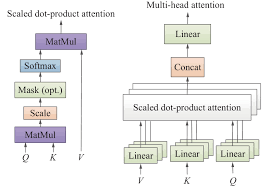
\includegraphics[width=0.80\linewidth]{figures/bcg/attention.png}
    \caption{Illustration of (a) scaled dot-product self-attention, (b) multi-head self-attention, and (c) cross-attention. In cross-attention, queries $\mathbf{Q}$ are projected from the visual feature sequence while keys $\mathbf{K}$ and values $\mathbf{V}$ are projected from the conditioning text embedding sequence $\mathbf{C}$, enabling each spatial position to selectively aggregate information from the text tokens.}
    \label{fig:attention_mechanisms}
\end{figure}

\section{The Transformer Architecture}
\label{sec:transformer}

The Transformer architecture, introduced by Vaswani et al.\ \cite{vaswani2017attention}, constitutes a paradigm shift in the design of deep neural networks for sequence modelling. Prior to its introduction, the dominant approaches for processing sequential data relied on recurrent neural networks (RNNs) and their gated variants, such as Long Short-Term Memory networks (LSTMs) \cite{hochreiter1997long} and Gated Recurrent Units (GRUs) \cite{cho2014learning}. These architectures suffer from an inherent sequential computation bottleneck: hidden states must be propagated step-by-step along the temporal axis, which prevents efficient parallelisation and impedes the capture of long-range dependencies due to vanishing gradient phenomena. The Transformer addresses both limitations by dispensing with recurrence entirely and replacing it with a mechanism of \emph{scaled dot-product attention}, enabling each position in a sequence to attend directly to every other position in a single computational step.

Formally, the core operation of the Transformer is the \emph{multi-head self-attention} mechanism. Given an input sequence represented as a matrix $\mathbf{X} \in \mathbb{R}^{n \times d_{\text{model}}}$, where $n$ is the sequence length and $d_{\text{model}}$ is the model dimensionality, three distinct linear projections produce the query, key, and value matrices:
\begin{equation}
    \mathbf{Q} = \mathbf{X}\mathbf{W}^Q, \quad
    \mathbf{K} = \mathbf{X}\mathbf{W}^K, \quad
    \mathbf{V} = \mathbf{X}\mathbf{W}^V,
    \label{eq:qkv}
\end{equation}
where $\mathbf{W}^Q, \mathbf{W}^K \in \mathbb{R}^{d_{\text{model}} \times d_k}$ and $\mathbf{W}^V \in \mathbb{R}^{d_{\text{model}} \times d_v}$ are learnable weight matrices. The attention output is then computed as:
\begin{equation}
    \text{Attention}(\mathbf{Q}, \mathbf{K}, \mathbf{V}) = \text{softmax}\!\left(\frac{\mathbf{Q}\mathbf{K}^\top}{\sqrt{d_k}}\right)\mathbf{V},
    \label{eq:attention}
\end{equation}
where the scaling factor $\sqrt{d_k}$ prevents the inner products from growing excessively large in magnitude, which would saturate the softmax function into near-zero gradient regions. In practice, multi-head attention runs $h$ parallel attention heads, each operating in a lower-dimensional subspace of dimension $d_k = d_v = d_{\text{model}} / h$, and their outputs are concatenated and linearly projected back to $d_{\text{model}}$:
\begin{equation}
    \text{MultiHead}(\mathbf{Q}, \mathbf{K}, \mathbf{V}) =
    \text{Concat}(\text{head}_1, \ldots, \text{head}_h)\,\mathbf{W}^O,
    \label{eq:multihead}
\end{equation}
where $\text{head}_i = \text{Attention}(\mathbf{X}\mathbf{W}_i^Q, \mathbf{X}\mathbf{W}_i^K, \mathbf{X}\mathbf{W}_i^V)$ and $\mathbf{W}^O \in \mathbb{R}^{h d_v \times d_{\text{model}}}$. This multi-head formulation allows the model to jointly attend to information from different representation subspaces at different positions, enriching the learned representations.

Each Transformer layer consists of two sub-layers: (i) the multi-head self-attention mechanism defined above and (ii) a position-wise feed-forward network (FFN) applied independently to each sequence position:
\begin{equation}
    \text{FFN}(\mathbf{z}) = \max(0, \mathbf{z}\mathbf{W}_1 + \mathbf{b}_1)\mathbf{W}_2 + \mathbf{b}_2,
    \label{eq:ffn}
\end{equation}
where $\mathbf{W}_1 \in \mathbb{R}^{d_{\text{model}} \times d_{\text{ff}}}$, $\mathbf{W}_2 \in \mathbb{R}^{d_{\text{ff}} \times d_{\text{model}}}$, and $d_{\text{ff}}$ is typically set to $4 d_{\text{model}}$. Residual connections \cite{he2016deep} wrap each sub-layer, followed by Layer Normalisation \cite{ba2016layer}, producing the standard pre-norm or post-norm Transformer block. Because the attention mechanism is inherently permutation-equivariant and thus insensitive to the order of input elements, positional information must be explicitly injected. The original formulation uses fixed sinusoidal encodings, though learned positional embeddings and more sophisticated relative positional schemes have been subsequently proposed \cite{shaw2018self, su2024roformer}.

The self-attention computation has a time and memory complexity of $\mathcal{O}(n^2 d_{\text{model}})$ with respect to sequence length $n$, which poses scalability challenges for long sequences. This quadratic bottleneck has motivated a rich body of work on efficient attention variants, including sparse attention \cite{child2019generating}, linear attention approximations \cite{katharopoulos2020transformers}, and hierarchical attention schemes. Notwithstanding this limitation, the Transformer has become the \emph{de facto} backbone for a broad range of tasks spanning natural language processing, speech, and, increasingly, computer vision and generative modelling, owing to its strong inductive biases towards long-range dependency modelling and its excellent scalability with respect to model size and training data.

% ============================================================
%  Section: Vision Transformers (ViT)
% ============================================================

\section{Vision Transformers}
\label{sec:vit}

The extension of the Transformer architecture to the visual domain was systematically explored by Dosovitskiy et al.\ \cite{dosovitskiy2020image}, who demonstrated that a pure Transformer applied directly to sequences of image patches can achieve competitive or superior performance compared to convolutional neural networks (CNNs) on image recognition benchmarks, provided that sufficient training data are available. This model, known as the Vision Transformer (ViT), challenged the long-standing dominance of convolutional architectures in computer vision and stimulated a proliferation of Transformer-based methods across discriminative and generative visual tasks alike.

\begin{figure}[ht]
    \centering
    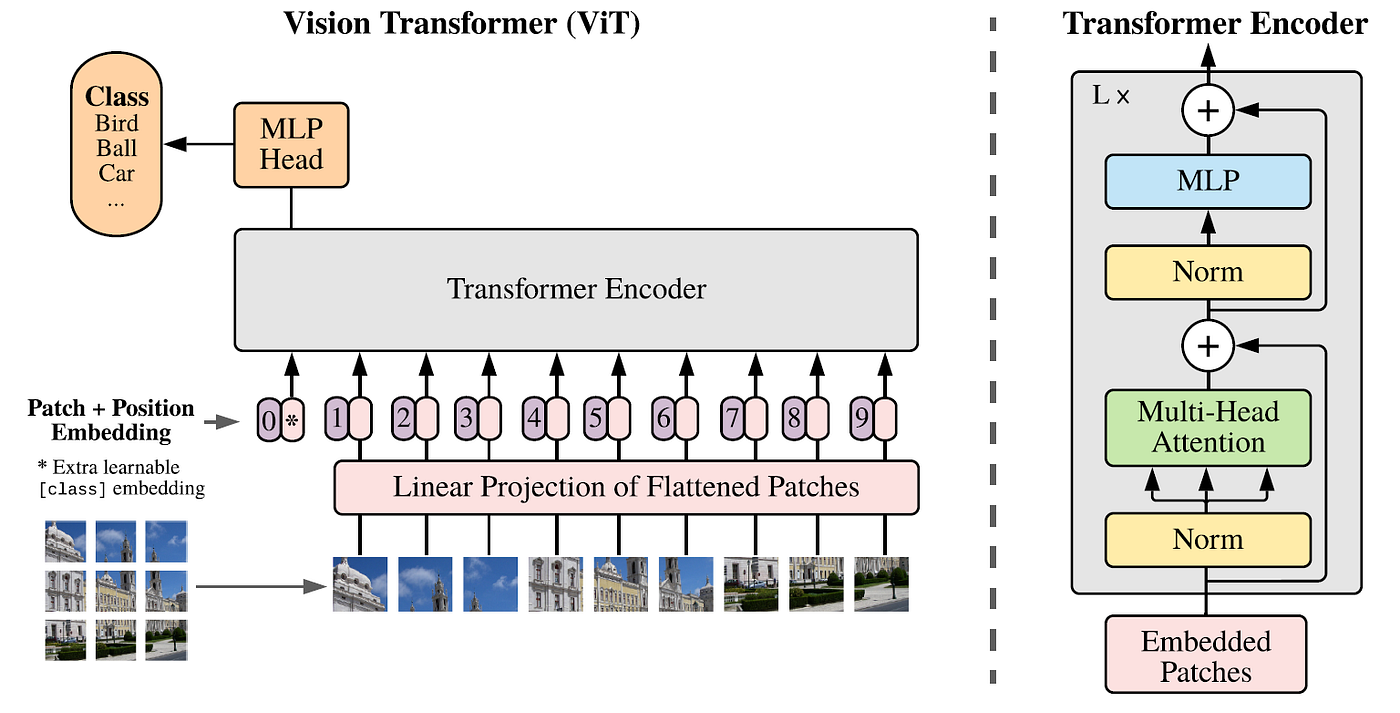
\includegraphics[width=0.85\linewidth]{figures/bcg/VIT.png}
    \caption{Overview of the Vision Transformer (ViT) architecture. An input image is partitioned into a grid of fixed-size patches, each linearly projected into a patch embedding. A learnable \texttt{[CLS]} token is prepended, positional embeddings are added, and the resulting sequence is processed by a stack of standard Transformer encoder blocks. The representation at the \texttt{[CLS]} token is used for classification. Figure adapted from \cite{dosovitskiy2020image}.}
    \label{fig:vit_architecture}
\end{figure}

% ============================================================
%  Subsection: Patch Embeddings and Positional Encoding
% ============================================================

\subsection{Patch Embeddings and Positional Encoding}
\label{subsec:patch_embeddings}

The principal challenge in applying Transformers to images lies in managing the computational cost of the quadratic attention mechanism. A raw image $\mathbf{x} \in \mathbb{R}^{H \times W \times C}$, if naively unrolled into a sequence of individual pixels, would yield a sequence of length $n = HW$, rendering self-attention computationally intractable for any practical image resolution. ViT resolves this by partitioning the image into a grid of non-overlapping patches of fixed size $P \times P$, resulting in $n = HW / P^2$ patches. Each patch $\mathbf{x}_i \in \mathbb{R}^{P^2 C}$ is then linearly projected into a $d_{\text{model}}$-dimensional embedding space via a learnable matrix $\mathbf{E} \in \mathbb{R}^{P^2 C \times d_{\text{model}}}$:
\begin{equation}
    \mathbf{z}_i^{(0)} = \mathbf{x}_i \mathbf{E} + \mathbf{e}_i^{\text{pos}},
    \quad i = 1, \ldots, n,
    \label{eq:patch_embedding}
\end{equation}
where $\mathbf{e}_i^{\text{pos}} \in \mathbb{R}^{d_{\text{model}}}$ is the positional embedding associated with the $i$-th position. Equivalently, the linear projection $\mathbf{E}$ can be implemented as a strided $P \times P$ convolution with $d_{\text{model}}$ output channels and stride $P$, which establishes a conceptual bridge to convolutional feature extraction.

A learnable classification token $\mathbf{z}_{\text{cls}} \in \mathbb{R}^{d_{\text{model}}}$, prepended to the patch sequence following the BERT convention \cite{devlin2019bert}, aggregates global image information through the attention mechanism. The full input sequence to the Transformer encoder is thus:
\begin{equation}
    \mathbf{Z}^{(0)} = \left[\mathbf{z}_{\text{cls}};\, \mathbf{z}_1^{(0)};\, \ldots;\, \mathbf{z}_n^{(0)}\right] \in \mathbb{R}^{(n+1) \times d_{\text{model}}}.
    \label{eq:vit_input}
\end{equation}
This sequence is then processed by $L$ stacked Transformer encoder blocks, each applying multi-head self-attention as described in Section~\ref{sec:transformer}, followed by a layer-normalised FFN with residual connections.

Positional encoding in ViT is typically realised through \emph{learned} 1D positional embeddings $\{\mathbf{e}_i^{\text{pos}}\}_{i=0}^{n}$, one for each patch position (plus the class token). Empirical comparisons reported in \cite{dosovitskiy2020image} indicate that 1D learned embeddings perform comparably to 2D-aware positional schemes for standard image resolutions, suggesting that the Transformer is capable of inferring 2D spatial relationships from 1D position information given sufficient data. More recent work has proposed relative positional encodings \cite{shaw2018self} and rotary positional embeddings (RoPE) \cite{su2024roformer} for ViT-style models, particularly to improve generalisation to image resolutions not seen during training — a practically important property for generative applications where spatial resolution may vary.

% ============================================================
%  Subsection: Scalability and Inductive Bias
% ============================================================

\subsection{Scalability and Inductive Bias}
\label{subsec:vit_scalability}

A defining characteristic of ViT relative to CNN-based architectures is its substantially weaker set of built-in inductive biases. Convolutional networks impose locality (each filter operates on a spatially contiguous receptive field), translation equivariance (a feature detector applied at one spatial location is reused across the entire feature map), and weight sharing. These structural priors are highly effective for natural image data and enable CNNs to generalise well even in data-limited regimes. The Transformer, in contrast, makes no structural assumptions about the spatial arrangement of its input tokens: every pair of patch tokens can interact with every other pair through the global attention mechanism, irrespective of their spatial distance. This architectural agnosticism is a double-edged property: it renders the model highly expressive and capable of capturing global dependencies that local convolutions cannot model efficiently, but it also necessitates substantially larger training datasets to learn the relevant spatial regularities that convolutional architectures acquire as an architectural prior.

This interplay between inductive bias and data scale is reflected empirically in the scaling behaviour of ViT. When trained on moderately sized datasets such as ImageNet-1k (${\sim}1.2$ million images), ViT lags behind well-regularised CNNs such as ResNet and EfficientNet \cite{he2016deep, tan2019efficientnet} in classification accuracy. However, when pre-trained on substantially larger corpora — in the order of hundreds of millions or billions of images — ViT models consistently outperform CNN counterparts \cite{dosovitskiy2020image, zhai2022scaling}. This observation motivates a shift in the design philosophy for large-scale vision models: rather than engineering architectural priors, one invests in data and compute, relying on the expressivity of the attention mechanism to discover the relevant structure from data.

The scalability of ViT is further underscored by the near-linear relationship between model capacity and downstream performance observed across multiple orders of magnitude in parameter count, from ViT-Small (${\sim}22$M parameters) through ViT-Base (${\sim}86$M) and ViT-Large (${\sim}307$M) to ViT-Huge (${\sim}632$M) and beyond \cite{zhai2022scaling}. This predictable scaling behaviour stands in contrast to CNN architectures, for which performance improvements tend to saturate more rapidly with increasing depth or width. Consequently, ViT has become the preferred backbone for foundation model pre-training in vision, underpinning models such as DINO \cite{caron2021emerging}, MAE \cite{he2022masked}, and CLIP \cite{radford2021learning}, all of which are directly relevant to the construction of powerful visual representations for downstream generative tasks.

% ============================================================
%  Subsection: Adapting ViT to Generative Tasks
% ============================================================

\subsection{Adapting ViT to Generative Tasks}
\label{subsec:vit_generative}

The success of ViT as a discriminative backbone has prompted extensive investigation into its utility as a backbone for generative modelling. This adaptation is non-trivial, as generative models impose architectural requirements that differ substantially from classification: they must produce spatially coherent, high-resolution outputs, and they must condition their generation on auxiliary signals such as class labels, text embeddings, or noisy latent states. Several strategies have emerged for repurposing the ViT architecture in this setting.

The most direct adaptation employs ViT as the denoising network within a diffusion model framework. The Diffusion Transformer (DiT), proposed by Peebles and Xie \cite{peebles2023scalable}, replaces the U-Net backbone conventionally used in denoising diffusion probabilistic models \cite{ho2020denoising} with a pure Transformer operating on sequences of latent image patches. DiT operates in the latent space of a pre-trained variational autoencoder (VAE), accepting as input the noisy latent $\mathbf{z}_t \in \mathbb{R}^{h \times w \times c}$ at diffusion timestep $t$, which is tokenised into a sequence of $n = hw/P^2$ patch tokens. Conditioning on the diffusion timestep $t$ and an optional class label $y$ is achieved through \emph{adaptive layer normalisation} (adaLN), wherein the scale and shift parameters of each layer normalisation are predicted by a small MLP applied to the sum of the timestep embedding and the class embedding:
\begin{equation}
    \text{adaLN}(\mathbf{h}, t, y) = \boldsymbol{\gamma}(t, y) \odot \frac{\mathbf{h} - \mu(\mathbf{h})}{\sigma(\mathbf{h})} + \boldsymbol{\beta}(t, y),
    \label{eq:adaln}
\end{equation}
where $\boldsymbol{\gamma}(t, y), \boldsymbol{\beta}(t, y) \in \mathbb{R}^{d_{\text{model}}}$ are the predicted scale and shift vectors, $\odot$ denotes element-wise multiplication, and $\mu$, $\sigma$ denote the mean and standard deviation computed over the feature dimension. This conditioning mechanism is more expressive than simple token concatenation and has been shown to be critical for the quality of conditional image synthesis.

\begin{figure}[ht]
    \centering
    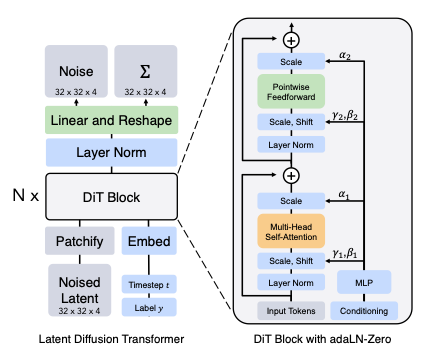
\includegraphics[width=0.85\linewidth]{figures/bcg/DIT-ADA.png}
    \caption{Schematic of a DiT block with adaptive layer normalization (adaLN). Conditioning signals from the diffusion timestep embedding and optional class label are used to modulate the layer normalization parameters $\boldsymbol{\gamma}$ and $\boldsymbol{\beta}$, providing flexible conditional control over the denoising process \cite{peebles2023scalable}.}
    \label{fig:dit_block}
\end{figure}

DiT exhibits the same favourable scaling properties as discriminative ViT: larger models trained for longer consistently achieve lower FID scores on class-conditional ImageNet generation, with DiT-XL/2 (trained at $256 \times 256$ resolution) surpassing all prior diffusion models including those based on U-Net backbones \cite{peebles2023scalable}. This scalability is particularly germane to the subject of the present thesis, as the Transformer backbone makes DiT an attractive target for knowledge distillation: the clean, modular structure of Transformer layers facilitates the design of intermediate feature-matching objectives, and the availability of a family of models at different scales (DiT-S, DiT-B, DiT-L, DiT-XL) provides natural student-teacher pairs that share an identical architectural template, differing only in depth and width.

Beyond DiT, other generative Transformer variants have been proposed. The U-ViT architecture \cite{bao2023all} hybridises the U-Net skip-connection topology with a Transformer backbone, introducing long skip connections between shallow and deep Transformer blocks to facilitate multi-scale feature propagation — a design motivated by the observation that low-frequency spatial information is most effectively communicated through direct shortcuts rather than through the deep processing stack. More recently, Flux and related flow-matching models \cite{lipman2022flow, esser2024scaling} have adopted Transformer-based backbones with multi-modal attention streams, enabling joint processing of image and text tokens within a unified attention computation. These architectures represent the current state of the art in text-to-image synthesis and are directly relevant to the distillation methodologies examined in Chapter~\ref{chap:knowledge_distillation}.

% ================================================================
% SECTION: The Just Image Transformer (JiT)
% ================================================================

\section{The Just Image Transformer (JiT)}
\label{sec:jit}

The Just image Transformer (JiT), introduced by \cite{li2025jit}, represents a principled return to the foundational objective of denoising generative models: directly predicting clean data rather than noise or a noised quantity. Despite the apparent simplicity of this design choice, it carries profound consequences for how neural networks handle high-dimensional image spaces. The JiT framework demonstrates that a plain Vision Transformer (ViT) operating directly on raw pixel patches — without any latent tokenizer, adversarial loss, perceptual loss, or self-supervised pre-training — can serve as a powerful and competitive generative backbone, provided the network is tasked with predicting the clean image $\bm{x}$ rather than the noise $\bm{\epsilon}$ or the flow velocity $\bm{v}$. This section details the theoretical motivation underpinning this design philosophy, the architectural choices that realise it, and the diffusion and flow-matching formulation within which JiT operates.

% ----------------------------------------------------------------
\subsection{The Manifold Assumption and the x-Prediction}
\label{subsec:jit_manifold}

A central premise of the JiT framework is the \emph{manifold hypothesis}, a long-standing conjecture in machine learning and statistics asserting that high-dimensional observational data, such as natural images, reside approximately on a low-dimensional nonlinear manifold embedded within the ambient observation space \cite{chapelle2006semi, carlsson2009topology, roweis2000nonlinear, tenenbaum2000global}. Formally, if $\bm{x} \in \mathbb{R}^D$ denotes a natural image of dimensionality $D$ (e.g., $D = 256 \times 256 \times 3 = 196{,}608$ for a colour image), the manifold hypothesis posits the existence of an intrinsic dimension $d \ll D$ such that the data distribution $p_{\mathrm{data}}(\bm{x})$ is supported on a $d$-dimensional submanifold $\mathcal{M} \subset \mathbb{R}^D$.

The implications of this hypothesis for diffusion model training are stark and have been largely overlooked in prior literature. In a standard Gaussian diffusion process, the noised intermediate variable at time $t$ is:
\begin{equation}
    \bm{z}_t = a_t \bm{x} + b_t \bm{\epsilon},
    \label{eq:jit_noisy}
\end{equation}
where $\bm{\epsilon} \sim \mathcal{N}(\bm{0}, \bm{I})$ is pure Gaussian noise and $a_t, b_t \in \mathbb{R}$ are pre-defined noise schedule coefficients. While the clean image $\bm{x}$ lies approximately on $\mathcal{M}$, both the noise $\bm{\epsilon}$ and the flow velocity $\bm{v} = \bm{x} - \bm{\epsilon}$ are inherently distributed across the full ambient space $\mathbb{R}^D$, as they involve an isotropic Gaussian component that fills the entire high-dimensional space \cite{vincent2010stacked}. This distinction is illustrated schematically in Figure~\ref{fig:jit_manifold}.

\begin{figure}[ht]
    \centering
    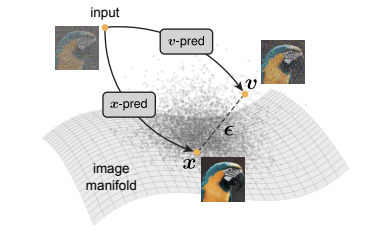
\includegraphics[width=0.72\linewidth]{figures/bcg/Manifold.png}
    \caption{c. A clean image $\bm{x}$ resides approximately on the low-dimensional data manifold $\mathcal{M}$ embedded within the high-dimensional pixel space $\mathbb{R}^D$. In contrast, the noise $\bm{\epsilon}$ and flow velocity $\bm{v} = \bm{x} - \bm{\epsilon}$ are off-manifold, distributed throughout $\mathbb{R}^D$. Training a network to predict $\bm{x}$ ($\bm{x}$-prediction) is therefore fundamentally different from training it to predict $\bm{\epsilon}$ or $\bm{v}$ (adapted from \cite{li2025jit}).}
    \label{fig:jit_manifold}
\end{figure}

This geometric insight has a direct consequence for neural network capacity. A network that must predict $\bm{\epsilon}$ is compelled to faithfully represent a full-dimensional Gaussian vector; it must retain all $D$ degrees of freedom of the noise, since any loss of information corrupts the prediction. In contrast, a network predicting $\bm{x}$ need only capture the $d$-dimensional structure of the data manifold and suppress the off-manifold noise components. Remarkably, this implies that even an \emph{under-capacity} network — one whose hidden dimension is smaller than the ambient dimension $D$ — can still perform $\bm{x}$-prediction effectively, because the information it must preserve is intrinsically low-dimensional.

\cite{li2025jit} verify this claim through a controlled toy experiment. A $d$-dimensional latent variable $\hat{\bm{x}} \in \mathbb{R}^d$ is embedded into an observed space of dimension $D \gg d$ via a fixed, randomly drawn column-orthogonal projection matrix $P \in \mathbb{R}^{D \times d}$, yielding $\bm{x} = P\hat{\bm{x}}$. A five-layer ReLU multilayer perceptron (MLP) with 256 hidden units is then trained as a generative model under $\bm{x}$-, $\bm{\epsilon}$-, and $\bm{v}$-prediction, all using the flow velocity loss (detailed in Section~\ref{subsec:jit_diffusion}). For small $D$ (e.g., $D = 2$ or $D = 8$), all three prediction modes perform reasonably. However, as $D$ increases to 16 and catastrophically to $D = 512$, $\bm{\epsilon}$-prediction and $\bm{v}$-prediction degrade severely, while $\bm{x}$-prediction continues to succeed — even though the MLP is strictly under-complete relative to the ambient space. This empirical finding is consistent with the manifold-theoretic argument: only $\bm{x}$-prediction respects the intrinsic dimensionality of the data, freeing the network from having to model the full high-dimensional noise distribution.

The broader context for this distinction can be traced to the prior literature on denoising autoencoders (DAEs) \cite{vincent2008extracting, vincent2010stacked}, where directly predicting clean data from corrupted observations was explicitly motivated by the manifold assumption. However, when \cite{ho2020denoising} demonstrated that $\bm{\epsilon}$-prediction dramatically outperformed $\bm{x}$-prediction within the DDPM framework, the field largely abandoned direct clean-image prediction. \cite{li2025jit} argue that this historical choice was appropriate in lower-dimensional regimes (e.g., latent spaces of dimensionality $\sim 64$–$256$ per token) where the capacity constraint is not binding, but becomes critically detrimental in the high-dimensional pixel space, where per-patch dimensionalities can reach 768 or 3072 depending on the patch size.

Furthermore, popular remedies for the high-dimensionality problem — such as reweighting the training loss, shifting the noise schedule, or increasing the network width — are shown by \cite{li2025jit} to be insufficient. Reweighting adjusts which noise levels receive more gradient signal but does not alter the fundamental capacity requirement for noise prediction. Increasing the network width proportionally to the token dimension rapidly becomes computationally intractable as resolution and patch size grow. The only principled remedy, JiT argues, is to change the prediction target itself.

% ----------------------------------------------------------------
\subsection{Architecture Overview: A Self-Contained ViT}
\label{subsec:jit_architecture}

The architectural design of JiT deliberately eschews the layers of specialisation that have accumulated in modern diffusion pipelines. Contemporary state-of-the-art image generators typically rely on a cascade of components: a pre-trained variational autoencoder (VAE) or vector-quantised tokeniser to project images into a compact latent space \cite{rombach2022ldm}, followed by adversarial or perceptual auxiliary losses drawn from pre-trained discriminators or classifiers \cite{goodfellow2014generative, zhang2018unreasonable}, and increasingly on self-supervised representation alignment objectives \cite{chen2024repa}. JiT eliminates all of these, operating entirely in raw pixel space with a single training objective and no external supervisory signal.

Formally, let $\bm{x} \in \mathbb{R}^{H \times W \times C}$ denote an input image of spatial dimensions $H \times W$ and $C = 3$ colour channels. JiT divides the image into non-overlapping square patches of side length $p$, yielding a sequence of $N = \frac{H}{p} \times \frac{W}{p}$ tokens, each of dimension $p^2 C$. For the canonical JiT/16 and JiT/32 configurations benchmarked on ImageNet at $256 \times 256$ and $512 \times 512$ resolutions respectively, the per-token dimensionalities are:
\begin{equation}
    d_{\text{token}} = p^2 C = \begin{cases} 16^2 \times 3 = 768 & \text{(JiT/16 at } 256 \times 256\text{)}, \\ 32^2 \times 3 = 3072 & \text{(JiT/32 at } 512 \times 512\text{)}. \end{cases}
    \label{eq:jit_token_dim}
\end{equation}
These dimensionalities are comparable to or substantially larger than those encountered in standard latent diffusion pipelines, where per-token latent dimensionalities are typically 4–16 \cite{rombach2022ldm, esser2024sd3}.

Each token is linearly projected into the Transformer's hidden dimension $d_{\text{model}}$ via a learned embedding matrix $W_e \in \mathbb{R}^{p^2 C \times d_{\text{model}}}$. Absolute sinusoidal positional embeddings are added, following the original ViT formulation \cite{dosovitskiy2021vit}. The sequence is then processed by $L$ standard Transformer blocks, each consisting of multi-head self-attention (MHSA) and a position-wise feed-forward network (FFN), with pre-normalisation via layer norm \cite{ba2016layer}. An output linear predictor $W_o \in \mathbb{R}^{d_{\text{model}} \times p^2 C}$ maps each output token back to a $p^2 C$-dimensional patch prediction. The complete pipeline is summarised in Figure~\ref{fig:jit_architecture}.

\begin{figure}[ht]
    \centering
    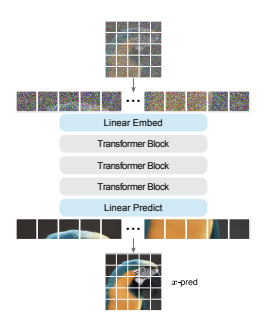
\includegraphics[width=0.78\linewidth]{figures/bcg/JIT.png}
    \caption{The JiT architecture. A noisy image $\bm{z}_t$ is patchified into a sequence of $N$ tokens, linearly embedded, processed by $L$ standard Transformer blocks conditioned on the diffusion time $t$ and class label $c$ via adaLN-Zero, and decoded back to pixel patches via a linear predictor. The direct output of the network is the clean image prediction $\hat{\bm{x}}_\theta$.}
    \label{fig:jit_architecture}
\end{figure}

Conditioning on the diffusion time step $t \in [0, 1]$ and, for class-conditional generation, on a class embedding $c$, is achieved through the adaptive layer normalisation with zero initialisation (adaLN-Zero) mechanism, as introduced by \cite{peebles2023dit}. In this formulation, time and class embeddings are combined and used to predict per-channel scale and shift parameters for the layer normalisation operations within each Transformer block, as well as a gating scalar applied to the residual branch outputs. The gate is initialised to zero, ensuring that the Transformer begins training as an identity mapping. Formally, for a hidden representation $\bm{h}$ at a given block:
\begin{equation}
    \bm{h} \leftarrow \bm{h} + \gamma \cdot \mathrm{Block}\!\left(\alpha \cdot \frac{\bm{h} - \mu}{\sigma} + \beta\right),
    \label{eq:adaln}
\end{equation}
where $\mu, \sigma$ are the layer-wise mean and standard deviation, and $\alpha, \beta, \gamma \in \mathbb{R}^{d_{\text{model}}}$ are affine parameters predicted from the joint time-class conditioning vector.

A notable finding from \cite{li2025jit} concerns the relationship between the network's hidden dimension $d_{\text{model}}$ and the per-patch dimension $d_{\text{token}}$. For $\bm{\epsilon}$- or $\bm{v}$-prediction, it has been suggested that the network width must at least match the token dimension, i.e., $d_{\text{model}} \geq d_{\text{token}}$, in order to avoid catastrophic failure \cite{TODO:chen2024highdim}. For JiT's $\bm{x}$-prediction, this constraint is relaxed: a bottleneck architecture in which $d_{\text{model}} < d_{\text{token}}$ can still perform well and may even improve generalisation, echoing classical results from manifold learning \cite{roweis2000nonlinear, tenenbaum2000global}. This bottleneck behaviour is consistent with the theoretical picture: if the true output is low-dimensional, the information compression induced by an under-complete hidden representation eliminates noise rather than distorting the signal. The authors exploit this with an optional bottleneck patch embedding that projects patches into a compressed 128-dimensional representation before the standard linear embedding, further reducing computational overhead without sacrificing generation quality.

The resulting architecture is intentionally minimal. It introduces no U-Net-style skip connections \cite{ronneberger2015unet}, no hierarchical multi-scale processing \cite{karras2018progressive}, no cross-attention to auxiliary conditioning sequences, and no dense convolutional layers. In this respect, JiT represents the most direct realisation of the Scalable Diffusion Transformers (DiT) \cite{peebles2023dit} philosophy: a clean, modality-agnostic ``Diffusion $+$ Transformer'' paradigm that operates on raw data tokens without domain-specific inductive biases.

% ----------------------------------------------------------------
\subsection{Diffusion Formulation and Flow Matching}
\label{subsec:jit_diffusion}

JiT adopts a flow-matching formulation \cite{lipman2022flow, liu2022flow, albergo2023building}, which can be interpreted as a specific instance of the broader diffusion modelling framework and provides a cleaner analytical foundation for understanding the relationships among the different prediction targets.

Let $\bm{x} \sim p_{\mathrm{data}}$ be a data sample and $\bm{\epsilon} \sim p_{\mathrm{noise}} = \mathcal{N}(\bm{0}, \bm{I})$ be independent Gaussian noise. A noisy interpolant at time $t \in [0, 1]$ is defined by the linear schedule:
\begin{equation}
    \bm{z}_t = t\bm{x} + (1-t)\bm{\epsilon},
    \label{eq:jit_interpolant}
\end{equation}
so that $\bm{z}_1 = \bm{x}$ (clean data) and $\bm{z}_0 \sim \mathcal{N}(\bm{0}, \bm{I})$ (pure noise). The time variable $t$ is sampled from a logit-normal distribution \cite{esser2024sd3}, i.e., $\mathrm{logit}(t) \sim \mathcal{N}(\mu, \sigma^2)$, which concentrates training signal in the intermediate noise levels that are most informative for learning.

The corresponding flow velocity is defined as the time-derivative of $\bm{z}_t$:
\begin{equation}
    \bm{v} \coloneqq \frac{d\bm{z}_t}{dt} = \bm{x} - \bm{\epsilon}.
    \label{eq:jit_velocity}
\end{equation}
Given this parametrisation, the three primary prediction targets — clean data, noise, and velocity — are algebraically related via Equations~\ref{eq:jit_interpolant} and \ref{eq:jit_velocity}:
\begin{equation}
    \bm{\epsilon}_\theta = \frac{\bm{z}_t - t\bm{x}_\theta}{1-t}, \qquad \bm{v}_\theta = \frac{\bm{x}_\theta - \bm{z}_t}{1-t},
    \label{eq:jit_derived}
\end{equation}
where $\bm{x}_\theta \coloneqq \mathrm{net}_\theta(\bm{z}_t, t)$ is the direct network output under $\bm{x}$-prediction. This shows that, regardless of the chosen prediction target, all three quantities can always be derived from any one of them, given $\bm{z}_t$ and $t$. A complete taxonomy of all nine possible combinations of (prediction space, loss space) in $\{\bm{x}, \bm{\epsilon}, \bm{v}\}$ is provided in \cite{li2025jit}.

For JiT, the training objective is the mean-squared error in the $\bm{v}$-space, applied to the $\bm{x}$-predicted network output — i.e., the $v$-loss with $x$-prediction:
\begin{equation}
    \mathcal{L}_{\mathrm{JiT}}(\theta) = \mathbb{E}_{t, \bm{x}, \bm{\epsilon}} \left\| \bm{v}_\theta(\bm{z}_t, t) - \bm{v} \right\|^2 = \mathbb{E}_{t, \bm{x}, \bm{\epsilon}} \frac{1}{(1-t)^2} \left\| \bm{x}_\theta(\bm{z}_t, t) - \bm{x} \right\|^2,
    \label{eq:jit_loss}
\end{equation}
where the right-hand side follows from substituting Equation~\ref{eq:jit_derived} into the $v$-loss. This reveals that the $v$-loss with $x$-prediction is equivalent to a reweighted $x$-loss with time-dependent weight $(1-t)^{-2}$, placing increasing emphasis on high-$t$ (low-noise) predictions as the sample approaches the clean data manifold. This loss-space and prediction-space decoupling is a key conceptual contribution of JiT's analysis, demonstrating that the \emph{combination} of loss weighting and prediction target must be considered jointly, not in isolation.

At inference, generation proceeds by numerically solving the following ordinary differential equation (ODE) from $t = 0$ to $t = 1$:
\begin{equation}
    \frac{d\bm{z}_t}{dt} = \bm{v}_\theta(\bm{z}_t, t),
    \label{eq:jit_ode}
\end{equation}
starting from $\bm{z}_0 \sim \mathcal{N}(\bm{0}, \bm{I})$. By default, \cite{li2025jit} employ a 50-step Heun solver \cite{karras2022edm} for numerical integration, which provides a favourable trade-off between generation fidelity and computational cost. At each step, the network produces an $\bm{x}$-prediction, from which the velocity $\bm{v}_\theta$ is derived via Equation~\ref{eq:jit_derived}, and the state $\bm{z}_t$ is advanced accordingly.

The JiT pipeline also supports classifier-free guidance (CFG) \cite{ho2022cfg} for class-conditional generation. During training, class labels are dropped with a fixed probability, and at inference the guided velocity is computed as:
\begin{equation}
    \tilde{\bm{v}}_\theta(\bm{z}_t, t, c) = \bm{v}_\theta(\bm{z}_t, t, \varnothing) + w \left[\bm{v}_\theta(\bm{z}_t, t, c) - \bm{v}_\theta(\bm{z}_t, t, \varnothing)\right],
    \label{eq:jit_cfg}
\end{equation}
where $c$ is the class label, $\varnothing$ denotes the null conditioning, and $w > 1$ is the guidance scale. \cite{li2025jit} further employ the CFG interval technique of \cite{kynkaanniemi2024applying}, which restricts CFG to the high-noise end of the trajectory (low $t$), a modification that consistently improves generation quality.

On the ImageNet benchmark at $256 \times 256$ and $512 \times 512$ resolutions, JiT achieves competitive Fréchet Inception Distance (FID) scores relative to contemporary latent diffusion models, despite operating entirely in pixel space and employing none of the auxiliary training components that such models rely upon. In configurations where the per-patch dimensionality exceeds the network's hidden dimension — the under-complete regime — $\bm{x}$-prediction maintains stable training and strong generation quality, while $\bm{\epsilon}$- and $\bm{v}$-prediction degrade catastrophically, with FID scores collapsing entirely. This empirical evidence, combined with the manifold-theoretic analysis outlined in Section~\ref{subsec:jit_manifold}, constitutes the core argument for $\bm{x}$-prediction as a principled design choice for high-dimensional generative modelling.

The relevance of JiT to the broader thesis theme of knowledge distillation in diffusion models is multifaceted. As a self-contained, tokeniser-free architecture, JiT presents a particularly clean setting for studying distillation: the absence of a pre-trained VAE removes one source of representational mismatch between teacher and student, and the manifold-theoretic justification for $\bm{x}$-prediction aligns naturally with consistency-based distillation objectives \cite{song2023consistency}, which also operate directly in the data space. The implications of the prediction target choice — and its interaction with student network capacity — are thus directly relevant to the distillation strategies discussed in Chapter~\ref{chap:knowledge_distillation}.
    \chapter{Knowledge Distillation}
\label{chap:knowledge_distillation}

% ─────────────────────────────────────────────────────────────────────────────
\section{Overview and Motivation}
\label{sec:kd_overview}
% ─────────────────────────────────────────────────────────────────────────────

The remarkable performance of modern deep neural networks is, in large part, a function of their scale.
Empirical evidence consistently demonstrates that increases in model depth, width, and training-data volume
yield systematic improvements across a wide range of tasks in computer vision, natural language processing,
and generative modelling \cite{kaplan2020scaling}.
Nevertheless, scale imposes a fundamental tension between accuracy and deployability: large models incur
prohibitive inference latency, memory footprint, and energy consumption that render them impractical in
resource-constrained settings such as mobile devices, embedded systems, and real-time applications.

Knowledge Distillation (KD) addresses this tension by transferring the predictive capability of a large,
high-capacity \emph{teacher} network $\mathcal{T}$ into a compact \emph{student} network $\mathcal{S}$,
without requiring the student to be trained from scratch on raw data alone.
The central insight, first systematically articulated by Hinton et al.\ \cite{hinton2015distilling}, is
that the soft output distributions produced by a well-trained teacher encode substantially richer
supervisory signals than the hard one-hot labels used in standard supervised learning.
For a classification problem over $C$ classes, the teacher produces a probability vector
$\mathbf{q}^{\mathcal{T}} \in \Delta^{C-1}$ via a temperature-scaled softmax,

\begin{equation}
    q^{\mathcal{T}}_c = \frac{\exp\!\left(z^{\mathcal{T}}_c / \tau\right)}{\sum_{j=1}^{C} \exp\!\left(z^{\mathcal{T}}_j / \tau\right)},
    \label{eq:soft_softmax}
\end{equation}

\noindent where $z^{\mathcal{T}}_c$ denotes the $c$-th logit of the teacher and $\tau \geq 1$ is a
temperature hyperparameter that softens the distribution, amplifying the information carried by
non-dominant classes.
The student is then trained to minimise a convex combination of the standard cross-entropy loss against
ground-truth labels and a distillation loss—typically the Kullback–Leibler divergence—against the teacher's
soft targets:

\begin{equation}
    \mathcal{L}_{\mathrm{KD}} = (1 - \alpha)\,\mathcal{L}_{\mathrm{CE}}\!\left(\mathbf{y},\, \mathbf{q}^{\mathcal{S}}\right)
    + \alpha \tau^2\, D_{\mathrm{KL}}\!\left(\mathbf{q}^{\mathcal{T}} \,\|\, \mathbf{q}^{\mathcal{S}}\right),
    \label{eq:kd_loss}
\end{equation}

\noindent where $\mathbf{y}$ is the one-hot label vector, $\mathbf{q}^{\mathcal{S}}$ is the student's
soft output evaluated at the same temperature $\tau$, and $\alpha \in [0,1]$ balances the two objectives.
The $\tau^2$ scaling factor compensates for the reduced magnitude of gradients at higher temperatures
\cite{hinton2015distilling}.

Beyond model compression, knowledge distillation has evolved into a versatile training paradigm.
It has been employed for domain adaptation \cite{Lopez-Paz2016unifying}, data-free compression
\cite{lopes2017data}, continual learning \cite{li2017learning}, and, most relevantly to the present work,
the acceleration of computationally intensive generative models such as diffusion models
\cite{salimans2022progressive, song2023consistency, luo2023lcm}.
The breadth of these applications motivates a systematic review of the classical distillation paradigms
before examining their specialised instantiation in the diffusion model context.

% ─────────────────────────────────────────────────────────────────────────────
\section{Classical Distillation Paradigms}
\label{sec:kd_classical}
% ─────────────────────────────────────────────────────────────────────────────

The literature on knowledge distillation can be taxonomised along two principal axes: the \emph{type} of
knowledge transferred (response-based, feature-based, or relation-based) and the \emph{training
scheme} employed (offline, online, or self-distillation) \cite{gou2021knowledge}.
The following subsections focus on the two paradigms most directly relevant to the distillation of
generative models: response-based and intermediate representation distillation.

% ─────────────────────────────────────────────────────────────────────────────
\subsection{Response-Based Distillation}
\label{subsec:kd_response}
% ─────────────────────────────────────────────────────────────────────────────

Response-based distillation, sometimes referred to as \emph{output distillation}, defines the knowledge to
be transferred exclusively through the final output layer of the teacher network.
In the classification setting, this corresponds to matching the soft class-probability vectors as
described by Equation~\ref{eq:kd_loss}.
The appeal of this formulation lies in its generality: it requires neither architectural alignment between
teacher and student nor access to intermediate activations, making it straightforwardly applicable across
heterogeneous model families.

From a probabilistic perspective, soft targets encode the teacher's \emph{dark knowledge}—the relative
likelihoods assigned to non-target classes that reflect inter-class similarities learned during training.
For instance, an image of the digit ``3'' may receive a non-negligible probability under the class ``8'',
reflecting shared visual structure.
Hard labels suppress this information entirely, whereas soft targets preserve it, providing a richer
inductive bias for the student \cite{hinton2015distilling}.

The temperature parameter $\tau$ in Equation~\ref{eq:soft_softmax} plays a critical regulatory role.
As $\tau \to \infty$, the soft distribution approaches the uniform distribution, reducing the distillation
signal to noise; as $\tau \to 1$, it collapses toward the teacher's argmax prediction, recovering the hard
label regime.
Empirically, intermediate values $\tau \in [2, 10]$ have been found to yield the best student performance
\cite{hinton2015distilling, tang2020understanding}.

In regression settings and generative modelling—where there is no discrete class structure—response-based
distillation takes the form of direct output matching.
Given a teacher output $\hat{\mathbf{y}}^{\mathcal{T}} = f_{\mathcal{T}}(\mathbf{x})$ for an input
$\mathbf{x}$, the student is trained under the mean squared error (MSE) objective,

\begin{equation}
    \mathcal{L}_{\mathrm{resp}} = \mathbb{E}_{\mathbf{x}}\!\left[\left\| f_{\mathcal{T}}(\mathbf{x}) - f_{\mathcal{S}}(\mathbf{x}) \right\|_2^2\right],
    \label{eq:response_mse}
\end{equation}

\noindent which constitutes the foundational loss used in methods such as Progressive Distillation for
diffusion models \cite{salimans2022progressive} and will be revisited in Section~\ref{sec:kd_diffusion}.

% ─────────────────────────────────────────────────────────────────────────────
\subsection{Intermediate Representation Distillation}
\label{subsec:kd_feature}
% ─────────────────────────────────────────────────────────────────────────────

Intermediate representation distillation—also referred to as \emph{feature-based} or
\emph{hint-based} distillation—augments the response-based objective by aligning the internal
representations of teacher and student at one or more intermediate layers.
The foundational contribution in this direction is FitNets \cite{romero2015fitnets}, which proposed
training the student to mimic the activation maps of a selected ``hint'' layer in the teacher,
enabling the transfer of richer, more structured knowledge than is available from the output alone.

Let $\mathbf{h}^{\mathcal{T}}_l \in \mathbb{R}^{d_{\mathcal{T}}}$ and
$\mathbf{h}^{\mathcal{S}}_{l'} \in \mathbb{R}^{d_{\mathcal{S}}}$ denote the feature maps at chosen
layers $l$ and $l'$ of the teacher and student, respectively.
Since the spatial and channel dimensions of these tensors generally differ, a learnable regressor
$r_\phi: \mathbb{R}^{d_{\mathcal{S}}} \to \mathbb{R}^{d_{\mathcal{T}}}$ (typically a convolutional
projection) is introduced to align the student features into the teacher's representation space.
The hint loss is then defined as

\begin{equation}
    \mathcal{L}_{\mathrm{hint}} = \mathbb{E}_{\mathbf{x}}\!\left[\left\| \mathbf{h}^{\mathcal{T}}_l(\mathbf{x}) - r_\phi\!\left(\mathbf{h}^{\mathcal{S}}_{l'}(\mathbf{x})\right) \right\|_2^2\right].
    \label{eq:hint_loss}
\end{equation}

A key motivation for feature-level supervision is that intermediate representations capture
\emph{structural} properties of the data—edges, textures, object parts—which are discarded in the
final output but are highly informative for guiding the student's internal computation.
This is particularly consequential for generative models, where the intermediate denoising activations
encode hierarchical semantic and perceptual information \cite{romero2015fitnets, zagoruyko2017paying}.

Subsequent work has explored a variety of alignment strategies beyond raw MSE matching.
Attention Transfer \cite{zagoruyko2017paying} matches spatial attention maps derived from feature
activations, defined as $\mathbf{A}_l = \text{vec}\!\left(\sum_c |\mathbf{h}^{\mathcal{T}}_{l,c}|^p\right)$
for $p \geq 1$, capturing the \emph{where} of network attention rather than the full activation volume.
Probabilistic Knowledge Transfer \cite{passalis2018learning} instead models the joint distribution of
feature activations and aligns it across teacher and student using kernel density estimation.
More recently, relational knowledge distillation \cite{park2019relational} has proposed transferring
structural relationships between instances—encoding pairwise or higher-order geometric configurations in
the representation space—rather than aligning individual activations.

\begin{figure}[ht]
    \centering
    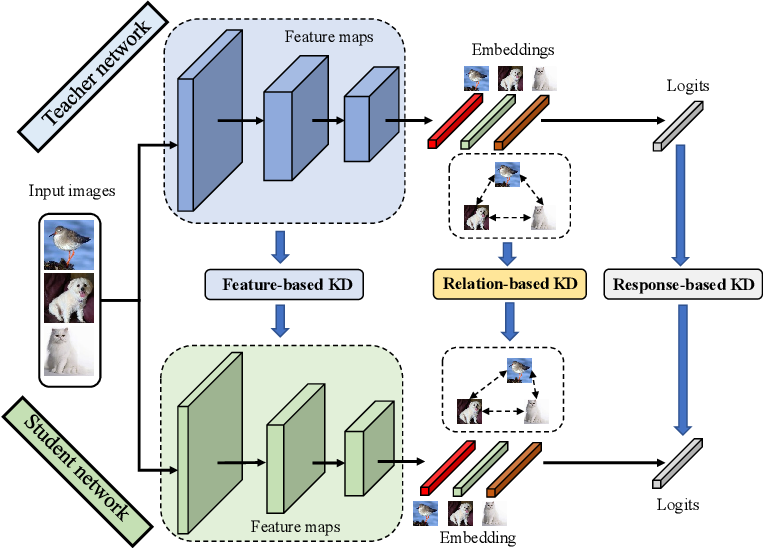
\includegraphics[width=0.88\linewidth]{figures/bcg/KD-M.png}
    \caption{Schematic comparison of response-based and intermediate representation distillation.
             In response-based distillation (left), only the final output of the teacher guides the
             student. In feature-based distillation (right), intermediate activation maps at selected
             layers are additionally aligned via a regression loss. A learnable projector $r_\phi$ is
             employed when the teacher and student feature dimensions are incompatible.}
    \label{fig:kd_paradigms}
\end{figure}

The selection of which layers to use for hint supervision is a non-trivial design decision.
Deeper layers tend to encode more semantically abstract features that are task-specific, while shallower
layers retain more generic, low-level visual information.
In practice, layer selection is often guided by architectural symmetry, cross-validation, or information-
theoretic criteria \cite{heo2019comprehensive}.
The combined training objective integrates both paradigms,

\begin{equation}
    \mathcal{L}_{\mathrm{total}} = \mathcal{L}_{\mathrm{task}} + \lambda_1 \mathcal{L}_{\mathrm{resp}} + \lambda_2 \mathcal{L}_{\mathrm{hint}},
    \label{eq:total_kd_loss}
\end{equation}

\noindent where $\lambda_1, \lambda_2 \geq 0$ are weighting hyperparameters balancing task performance,
output matching, and representational alignment.

% ─────────────────────────────────────────────────────────────────────────────
\section{Diffusion Model Distillation}
\label{sec:kd_diffusion}
% ─────────────────────────────────────────────────────────────────────────────

The application of knowledge distillation to diffusion models is motivated primarily by the high
computational cost of iterative sampling.
Standard Denoising Diffusion Probabilistic Models (DDPMs) \cite{ho2020denoising} require on the order
of $T \sim 1000$ sequential network function evaluations (NFEs) to generate a single sample, as the
reverse process progressively denoises a Gaussian variable $\mathbf{x}_T \sim \mathcal{N}(\mathbf{0},
\mathbf{I})$ through a learned Markov chain.
While accelerated samplers such as DDIM \cite{song2021denoising} and DPM-Solver \cite{lu2022dpm} reduce
the required NFEs to tens or dozens by exploiting deterministic or higher-order ODE integration,
further reduction to a handful of steps—or ideally a single step—without material quality degradation
requires a fundamentally different approach: distillation of the multi-step sampling trajectory into a
student that directly learns to approximate the full trajectory mapping.

\textbf{Progressive Distillation.}
Salimans and Ho \cite{salimans2022progressive} introduced Progressive Distillation (PD) as a response-
based distillation scheme applied iteratively to the diffusion sampling trajectory.
Given a teacher that executes $N$ denoising steps, the student is trained to match the teacher's
\emph{two-step} output in a \emph{single} step, effectively halving the number of required NFEs.
This procedure is applied repeatedly: the trained student is promoted to the teacher role, and a new
student is distilled with another 2$\times$ reduction, yielding a sequence of models requiring
$N, N/2, N/4, \ldots$ steps respectively.
The student's denoising network $\epsilon_\theta$ is trained under

\begin{equation}
    \mathcal{L}_{\mathrm{PD}} = \mathbb{E}_{t, \mathbf{x}_0, \boldsymbol{\epsilon}}\!\left[\omega(t) \left\| \hat{\mathbf{x}}_0^{\mathcal{T}}(\mathbf{x}_t) - \hat{\mathbf{x}}_0^{\mathcal{S}}(\mathbf{x}_t) \right\|_2^2\right],
    \label{eq:progressive_distillation}
\end{equation}

\noindent where $\hat{\mathbf{x}}_0^{\mathcal{T}}(\mathbf{x}_t)$ is the teacher's two-step prediction
of the clean image from the noisy input $\mathbf{x}_t$, $\hat{\mathbf{x}}_0^{\mathcal{S}}(\mathbf{x}_t)$
is the student's single-step prediction, and $\omega(t)$ is a time-step-dependent weighting function.
Progressive Distillation has demonstrated that image quality competitive with the teacher can be achieved
with as few as 4 NFEs, representing an over two-orders-of-magnitude reduction relative to the original
DDPM schedule.

\textbf{Consistency Distillation and Consistency Models.}
Song et al.\ \cite{song2023consistency} proposed Consistency Models, which are grounded in the
observation that all points along a deterministic probability flow ODE trajectory, conditioned on the same
final sample $\mathbf{x}_0$, must be mapped to the same clean image by the learned consistency function
$f_\theta(\mathbf{x}_t, t) \approx \mathbf{x}_0$.
Consistency Distillation (CD) trains the student by enforcing \emph{self-consistency} of adjacent
trajectory points: for two time steps $t > s$ connected by one step of the numerical ODE solver,

\begin{equation}
    \mathcal{L}_{\mathrm{CD}}(\theta, \theta^{-}) = \mathbb{E}_{t, \mathbf{x}_0}\!\left[\, d\!\left(f_\theta(\mathbf{x}_t,\, t),\; f_{\theta^{-}}(\hat{\mathbf{x}}_s,\, s)\right)\right],
    \label{eq:consistency_distillation}
\end{equation}

\noindent where $\hat{\mathbf{x}}_s$ is the one-step numerical estimate of $\mathbf{x}_s$ obtained from
$\mathbf{x}_t$ via a pre-trained diffusion teacher, $\theta^{-}$ are exponential moving average (EMA)
parameters used as the target network to stabilise training, and $d(\cdot, \cdot)$ is a
perceptual or $\ell_2$ distance metric.
Importantly, Consistency Models can also be trained in a teacher-free regime—Consistency Training
(CT)—by bootstrapping the target from the model's own EMA parameters, thus circumventing the need for a
pre-trained diffusion teacher altogether.

\textbf{Latent Consistency Models.}
Luo et al.\ \cite{luo2023lcm} extended the consistency distillation framework to the latent space of
pre-trained latent diffusion models (LDMs) \cite{rombach2022latent}, yielding Latent Consistency Models
(LCMs).
By operating in the compressed latent space of a variational autoencoder rather than in pixel space,
LCMs inherit both the high fidelity of LDMs and the inference efficiency of consistency distillation,
achieving competitive image quality with as few as 2–4 denoising steps on large-scale text-to-image
benchmarks.

The distillation methods described above share a common structural blueprint: a pre-trained diffusion
model serves as the teacher, providing trajectory or output supervision; a student of equal or smaller
capacity is trained to replicate this supervision in fewer function evaluations; and the quality of the
resulting student is evaluated via established metrics such as the Fréchet Inception Distance (FID)
\cite{heusel2017gans} and CLIP score \cite{radford2021learning}.
The specific choice of distillation paradigm—response-based trajectory matching, consistency
enforcement, or adversarial refinement via score distillation sampling \cite{poole2022dreamfusion}—
introduces distinct trade-offs between sample quality, training stability, and generality that will be
examined in depth in Chapter~\ref{chap:knowledge_distillation}.

\begin{figure}[ht]
    \centering
    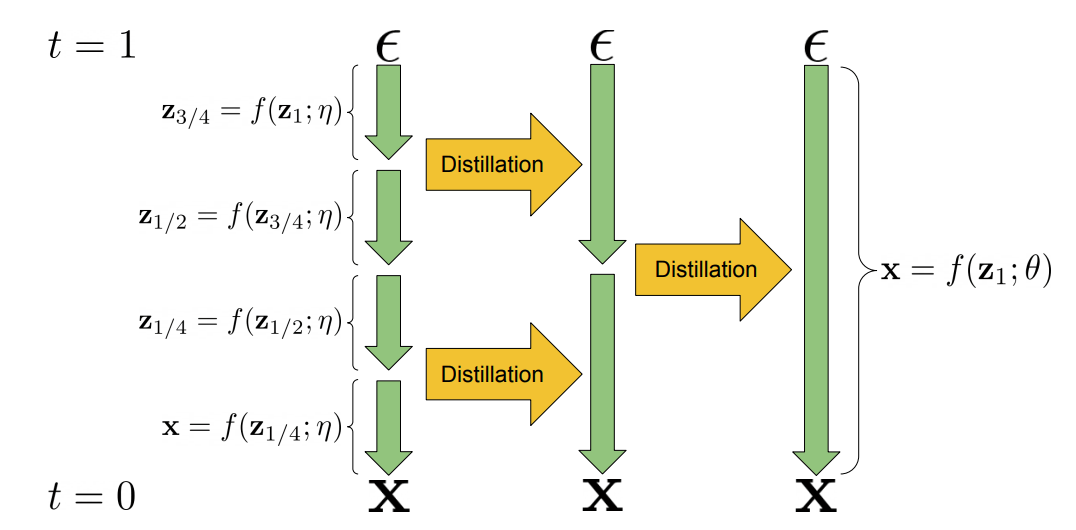
\includegraphics[width=0.92\linewidth]{figures/bcg/progressive_distillation.png}
    \caption{Conceptual overview of diffusion model distillation approaches.
             Progressive Distillation (top) iteratively halves the number of required sampling steps
             by matching two-step teacher outputs with single-step student predictions.
             Consistency Distillation (bottom) enforces self-consistency of all trajectory points
             mapping to the same clean sample $\mathbf{x}_0$, enabling one- or few-step generation.}
    \label{fig:diffusion_distillation_overview}
\end{figure}
\end{figure}
    \chapter{Our Distillation Framework for Pixel-Space Diffusion}
\label{chap:framework}

% ============================================================
\section{Framework Overview and Motivation}
\label{sec:framework_overview}
% ============================================================

The prevailing paradigm of knowledge distillation applied to diffusion models has been almost exclusively concerned with \emph{sampling acceleration}: given a fully trained teacher, a student is trained to reproduce the teacher's output in fewer denoising steps, thereby reducing the number of function evaluations (NFE) at inference time \cite{salimans2022progressive, song2023consistency, luo2023lcm}. While this line of work is practically valuable, it addresses a fundamentally different objective than the one pursued in this thesis. Sampling-acceleration methods do not alter the capacity or representational quality of the student model; a student that converges under such a scheme simply learns to approximate the teacher's multi-step trajectory in fewer steps, but it cannot surpass the teacher's generative quality ceiling at a fixed NFE. Our goal is orthogonal: we seek to \emph{improve the generative quality} of a smaller JiT model without modifying its inference-time architecture, parameter count, or computational cost. That is, for an identical deployment budget, we aim to produce a strictly higher-quality generative model by leveraging supervision from a larger, pretrained JiT teacher during training. The distillation signal is discarded at inference time; the student runs as a standalone model.

This quality-boosting objective is enabled by a property specific to JiT \cite{li2025jit}: it operates directly in pixel space. Unlike latent diffusion models \cite{rombach2022ldm}, whose denoising trajectories unfold over opaque, high-dimensional latent codes with no direct visual interpretation, JiT's intermediate states at every denoising timestep are actual noisy images — semantically grounded, spatially structured, and directly inspectable. This observability has a concrete consequence for distillation: the internal representations of JiT, including its multi-head self-attention maps and intermediate feature tensors, are dense, spatially coherent, and carry interpretable information about image structure at every point along the denoising trajectory. In latent-space models, by contrast, such intermediate representations encode statistics of an abstract embedding space, and their spatial correspondence to image content is indirect and architecture-dependent. The pixel-space setting thus exposes a richer and more supervisable knowledge structure, making JiT a uniquely suitable backbone for feature-level distillation.

Concretely, this thesis investigates three complementary distillation strategies applied within a unified teacher--student framework. The teacher is a larger, pretrained JiT variant with its weights held frozen throughout training. The student is a smaller JiT variant trained from scratch — or from an informed initialisation — under the combined supervision of the standard flow-matching objective and additional distillation losses derived from the teacher's internal representations. We conduct experiments on two benchmarks at different scales of difficulty: CIFAR-10 \cite{krizhevsky2009cifar}, where the teacher--student pair is JiT-S/2 (48.2M parameters) and JiT-T/2 (16.5M parameters), respectively; and ImageNet-1K \cite{russakovsky2015imagenet}, where the pair is JiT-B/16 (teacher) and JiT-S/16 (student). Full experimental details, training protocols, and quantitative results are reported in Chapter~\ref{chap:experiments}.

The three distillation strategies are as follows. First, the primary methodology is \emph{feature map distillation via ViTKD} (Section~\ref{sec:vitkd}), which transfers knowledge encoded in the intermediate hidden-state tensors of the teacher's transformer blocks. Second, \emph{attention map distillation} (Section~\ref{sec:attn_kd}) transfers the spatial attention routing patterns of the teacher — the learned structure governing how information flows between image patch tokens. Third, \emph{weight selection} (Section~\ref{sec:weight_selection}) serves as a complementary initialisation strategy rather than an online loss, seeding the student's parameters from a structured subset of the teacher's pretrained weights before any gradient update. A schematic overview of the full framework is illustrated in Figure~\ref{fig:framework_overview}.

\begin{figure}[ht]
    \centering
    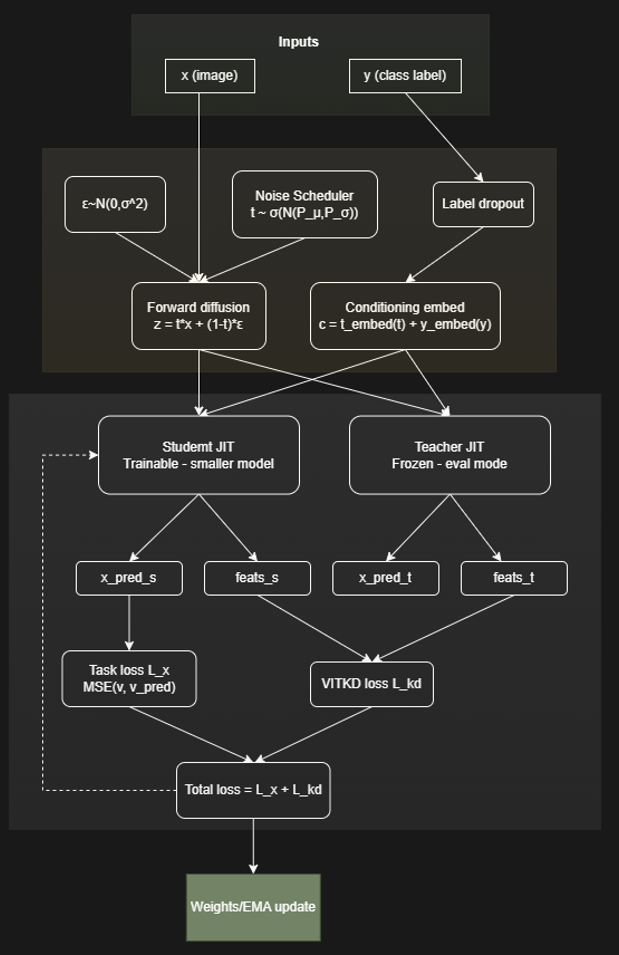
\includegraphics[width=0.92\linewidth]{figures/formula/training-loop.png}
    \caption{Overview of the proposed knowledge distillation framework. The teacher JiT model (larger variant) is frozen and processes the same noisy input as the student (smaller variant) at every training step. Three distillation signals are derived from the teacher: (i) intermediate feature maps from shallow and deep transformer blocks, used by the ViTKD loss; (ii) post-softmax self-attention weight matrices from the final $K$ blocks, used by the attention KD loss; and (iii) a structured subset of pretrained weights, used to initialise the student prior to training. The student is additionally supervised by the standard flow-matching denoising loss $\mathcal{L}_{\text{flow}}$. At inference time, only the student is used.}
    \label{fig:framework_overview}
\end{figure}


% ============================================================
\section{Feature Map Distillation via ViTKD}
\label{sec:vitkd}
% ============================================================

\subsection{Motivation: Feature Distillation for Vision Transformers}
\label{subsec:vitkd_motivation}

Feature-based knowledge distillation has a long history in the context of convolutional neural networks (CNNs), tracing back to the seminal FitNets framework \cite{romero2015fitnets}, which proposed to match intermediate feature maps between teacher and student networks via a regression objective. Subsequent works refined this idea through attention-based feature transfer \cite{zagoruyko2017paying}, relational feature distillation \cite{park2019relational}, and various forms of channel-wise or spatial normalisation \cite{heo2019comprehensive}. These methods, however, were designed with the specific inductive biases of CNNs in mind: hierarchical spatial resolution, local receptive fields, and feature maps with explicit channel-height-width structure. When applied naïvely to Vision Transformers \cite{dosovitskiy2020vit}, they tend to be ineffective or even detrimental, owing to the fundamental architectural differences: ViTs operate on a flat sequence of patch tokens with a fixed spatial resolution throughout, no pooling hierarchy, and feature representations that encode information in a distributed, non-local manner across the sequence dimension.

Responding to this gap, \cite{yang2022vitkd} conducted a systematic empirical study of feature distillation strategies tailored specifically to ViTs. Through a series of controlled ablations, they derived three practical guidelines that deviate substantially from CNN-era conventions. First, \emph{shallow transformer layers} are best distilled via direct mimicking: aligning the student's early hidden states to the teacher's counterparts through a simple learned linear projection, supervised by a mean squared error objective. In contrast to CNN practices, where shallow feature distillation is often less informative than deep feature distillation, shallow ViT layers attend to low-level structural patterns and positional relationships that are foundational to the subsequent processing of the sequence; transferring them directly proves highly beneficial. Second, \emph{deep transformer layers} are best distilled via a generative reconstruction objective: a fraction of the student's final-layer tokens are masked and replaced with a learned mask token, and a lightweight convolutional projector is trained to reconstruct the teacher's corresponding deep features at the masked positions. This forces the student to capture the global context and high-level semantic structure encoded in the teacher's final hidden states, rather than merely performing local point-wise regression. Third, a simple linear projection is sufficient for dimension alignment between teacher and student embedding spaces; elaborate multi-layer projection heads introduce unnecessary optimisation difficulty and degrade distillation performance. On ImageNet-1K image classification with DeiT architectures, this framework, termed ViTKD, yields consistent and significant improvements across multiple student sizes \cite{yang2022vitkd}.

The applicability of ViTKD to diffusion model distillation is non-trivial, but its core principles are well-motivated in this context. In JiT, the transformer blocks process patch token sequences derived directly from noisy pixel-space images, and the resulting feature representations are conditioned on both the class label $y$ and the continuous noise level $t$. Early blocks encode coarse low-level denoising patterns, positional structure, and texture statistics, while the final block aggregates global contextual information that determines the model's final velocity prediction $v_\theta(\mathbf{z}, t, y)$. Supervising the student's intermediate representations to match those of a larger teacher thus exerts pressure for the student to develop more accurate and better-calibrated internal models of the denoising process, which translates directly into higher generative quality.

\subsection{Adapting ViTKD to the Diffusion Setting}
\label{subsec:vitkd_adaptation}

Although the architectural backbone is shared — both the original ViTKD and our setting involve a pair of Vision Transformers of differing capacities — several non-trivial adaptations are required to apply ViTKD effectively to a conditional diffusion model. The central challenge is that, unlike a classification network whose internal representations are conditioned only on the input image, the hidden states of a diffusion model are explicitly conditioned on the noise level $t \in [0, 1]$. In JiT, this conditioning is implemented via adaptive layer normalisation (adaLN) \cite{peebles2023scalable}, in which each transformer block computes per-block shift and scale vectors from a conditioning signal $\mathbf{c} \in \mathbb{R}^{D}$ that fuses the timestep embedding and the class embedding. As a result, the statistical properties of the intermediate hidden states — their scale, orientation in embedding space, and distributional shape — vary substantially across the denoising trajectory. A plain linear alignment layer $\phi: \mathbb{R}^{D_S} \to \mathbb{R}^{D_T}$, as prescribed in the original ViTKD, is a static affine map that cannot account for this trajectory-dependent variation and may therefore produce a poorly calibrated distillation objective at certain noise levels.

To address this, we introduce a \textbf{timestep-conditioned alignment layer}, which we term \texttt{AdaLNAlign}. Rather than applying a bare linear projection, the aligned feature is modulated by an adaLN operation conditioned on the student's conditioning vector $\mathbf{c}$:
%
\begin{equation}
    \phi_i^{\text{AdaLN}}(\mathbf{F}_i^S, \mathbf{c}) = \left(1 + \boldsymbol{\gamma}_i(\mathbf{c})\right) \odot \mathbf{W}_i \mathbf{F}_i^S + \boldsymbol{\delta}_i(\mathbf{c}),
    \label{eq:adaln_align}
\end{equation}
%
where $\mathbf{F}_i^S \in \mathbb{R}^{B \times N \times D_S}$ denotes the student's feature tensor at shallow layer $i$, $\mathbf{W}_i \in \mathbb{R}^{D_T \times D_S}$ is a learnable linear projection, and the per-token shift and scale vectors $\boldsymbol{\delta}_i(\mathbf{c}), \boldsymbol{\gamma}_i(\mathbf{c}) \in \mathbb{R}^{B \times N \times D_T}$ are produced by a two-layer MLP applied to $\mathbf{c}$ and broadcast over the token dimension. The MLP's output layer is initialised to zero, ensuring that at the start of training the alignment degenerates to a plain linear projection, and the modulation is learned progressively. This design allows the alignment layer to dynamically rescale and shift the student's features according to the current noise level before computing the mimicking loss, thereby normalising out trajectory-induced distributional variation.

A second adaptation concerns the weighting of individual training samples in the distillation loss. At extreme noise levels, particularly for $t$ close to zero or one, the signal-to-noise ratio (SNR) of the noisy input $\mathbf{z} = t\mathbf{x} + (1-t)\mathbf{e}$ is either very high (nearly clean) or very low (nearly pure noise), and the gradients produced by the distillation loss at these regimes tend to be either trivially small or dominated by noise artefacts. To mitigate this, we adopt \textbf{Min-SNR-$\gamma$ loss weighting} \cite{hang2023efficient}, which assigns per-sample weights $w(t)$ based on the effective SNR of the training sample:
%
\begin{equation}
    \mathrm{SNR}(t) = \left( \frac{t}{1 - t} \right)^2, \qquad w(t) = \frac{\min\!\left(\mathrm{SNR}(t),\, \gamma\right)}{\gamma},
    \label{eq:snr_weight}
\end{equation}
%
where $\gamma > 0$ is a clipping hyperparameter that prevents samples with very high SNR from dominating the loss. When $\gamma = 0$, the weighting is disabled and all samples are treated uniformly. This weighting is applied to both the mimicking and generation components of the ViTKD loss.


\subsection{Shallow-Layer Mimicking Loss}
\label{subsec:vitkd_mimic}

The mimicking component of ViTKD operates on the output hidden states of the first two transformer blocks of both teacher and student. Let $\mathbf{F}_i^S \in \mathbb{R}^{B \times N \times D_S}$ and $\mathbf{F}_i^T \in \mathbb{R}^{B \times N \times D_T}$ denote the post-block feature tensors of the student and teacher at shallow layer $i \in \{0, 1\}$, respectively, where $B$ is the batch size, $N$ is the number of patch tokens, and $D_S$, $D_T$ are the respective embedding dimensions. When $D_S \neq D_T$, dimension alignment is required before computing the loss. Depending on whether timestep conditioning is enabled, the alignment is performed by either the \texttt{AdaLNAlign} module introduced in Equation~\eqref{eq:adaln_align} or a plain learned linear projection $\mathbf{W}_i \in \mathbb{R}^{D_T \times D_S}$. In both cases, the aligned student feature is denoted $\hat{\mathbf{F}}_i^S \in \mathbb{R}^{B \times N \times D_T}$.

The mimicking loss is then computed as a mean squared error between aligned student features and the corresponding teacher features, summed over the two shallow layers and normalised by batch size:
%
\begin{equation}
    \mathcal{L}_{\text{mimic}} = \frac{\alpha}{B} \sum_{i=0}^{1} \sum_{b=1}^{B} w(t_b) \cdot \left\| \hat{\mathbf{F}}_{i,b}^S - \mathbf{F}_{i,b}^T \right\|_F^2,
    \label{eq:loss_mimic}
\end{equation}
%
where $\alpha$ is a scalar loss weight, $w(t_b)$ is the Min-SNR-$\gamma$ weight for sample $b$ (equal to 1 when weighting is disabled), and $\|\cdot\|_F^2$ denotes the squared Frobenius norm over the token and channel dimensions. The alignment layers $\{\mathbf{W}_i\}_{i=0}^{1}$ are the only learnable parameters introduced by this component; they are trained jointly with the student network via backpropagation. The teacher features $\mathbf{F}_i^T$ are computed under \texttt{torch.no\_grad()} and treated as fixed targets.

In the JiT architecture, the first two transformer blocks operate on the patch embedding before the deeper adaLN-modulated blocks begin to integrate strong class and noise-level conditioning. Their outputs therefore reflect a relatively stable, low-level decomposition of the input, making them suitable targets for direct regression. The mimicking loss exerts a force that aligns the student's early computational pathway to the teacher's, promoting the development of analogous low-level feature detectors.


\subsection{Deep-Layer Generation Loss}
\label{subsec:vitkd_gen}

The generation component of ViTKD targets the output hidden states of the final transformer block of both teacher and student. Let $\mathbf{H}^S \in \mathbb{R}^{B \times N \times D_S}$ and $\mathbf{H}^T \in \mathbb{R}^{B \times N \times D_T}$ denote these deep features. The rationale for treating shallow and deep layers differently is that the final-block representations in a trained ViT encode high-level, globally integrated semantic information that is difficult to transfer via direct regression: a student with insufficient capacity may simply overfit to matching the teacher's final features locally without developing the underlying distributed processing structure required to produce them. The generation objective sidesteps this issue by introducing a reconstruction task under partial information, compelling the student to leverage global context rather than performing local point-wise imitation.

The procedure operates as follows. The student's deep features $\mathbf{H}^S$ are first linearly projected to the teacher's dimension: $\tilde{\mathbf{H}}^S = \mathbf{W}_{\text{deep}} \mathbf{H}^S$, where $\mathbf{W}_{\text{deep}} \in \mathbb{R}^{D_T \times D_S}$. A random binary mask $\mathbf{m} \in \{0, 1\}^{B \times N}$ is then sampled per batch, with each token independently masked with probability $\lambda \in (0, 1)$. Masked token positions in $\tilde{\mathbf{H}}^S$ are replaced with a shared learnable mask token $\boldsymbol{\mu} \in \mathbb{R}^{1 \times 1 \times D_T}$, broadcast over the batch and masked positions. The resulting partially-masked sequence is reshaped from its flat token representation $\mathbb{R}^{B \times N \times D_T}$ into a spatial grid $\mathbb{R}^{B \times D_T \times \sqrt{N} \times \sqrt{N}}$, passed through a lightweight convolutional projector consisting of two $3 \times 3$ convolutions with a ReLU nonlinearity, and then reshaped back to the token format. The generation loss is computed only on the masked positions, measuring how well the projector can reconstruct the teacher's deep features at those locations using the spatial context provided by the surrounding unmasked tokens:
%
\begin{equation}
    \mathcal{L}_{\text{gen}} = \frac{\beta}{B \lambda} \sum_{b=1}^{B} w(t_b) \cdot \left\| \left( \hat{\mathbf{H}}_b^S - \mathbf{H}_b^T \right) \odot \mathbf{m}_b \right\|_F^2,
    \label{eq:loss_gen}
\end{equation}
%
where $\hat{\mathbf{H}}_b^S$ denotes the projector output for sample $b$, $\mathbf{m}_b \in \{0,1\}^{N \times 1}$ is the per-sample mask broadcast over the channel dimension, $\beta$ is a scalar loss weight, and the $\lambda$ factor in the denominator normalises for the varying number of masked tokens. The mask is sampled uniformly at random without replacement using a noise-based shuffling procedure \cite{he2022masked}. In practice, $\lambda = 0.5$ is used as the default masking ratio, meaning that half of the student's deep tokens are masked per step.

The convolutional projector is the critical architectural element distinguishing the generation component from a second mimicking term: by requiring the model to spatially interpolate across masked positions using a $3 \times 3$ receptive field, it forces the student's projected features to encode local spatial coherence consistent with the teacher's global deep representation. This is particularly meaningful in the diffusion context, where the final-block features must ultimately support a spatially consistent velocity prediction across the entire image.

An ablation mode \texttt{mimic\_only} is provided, in which the generation loss is omitted entirely and only $\mathcal{L}_{\text{mimic}}$ is applied. This configuration is investigated experimentally in Chapter~\ref{chap:experiments} to isolate the contribution of each component.


\subsection{Total ViTKD Loss}
\label{subsec:vitkd_total}

The overall ViTKD distillation loss is the sum of the shallow-layer mimicking loss and the deep-layer generation loss:
%
\begin{equation}
    \mathcal{L}_{\text{ViTKD}} = \mathcal{L}_{\text{mimic}} + \mathcal{L}_{\text{gen}},
    \label{eq:loss_vitkd}
\end{equation}
%
where $\mathcal{L}_{\text{mimic}}$ and $\mathcal{L}_{\text{gen}}$ are as defined in Equations~\eqref{eq:loss_mimic} and~\eqref{eq:loss_gen}, respectively. The two terms are independently scaled by $\alpha$ and $\beta$, with default values $\alpha = 3 \times 10^{-5}$ and $\beta = 3 \times 10^{-6}$, reflecting the fact that the generation loss is applied to a smaller subset of tokens and its gradient norm would otherwise dominate at higher values. During training, $\mathcal{L}_{\text{ViTKD}}$ is added to the primary flow-matching denoising loss of the student, described in Section~\ref{sec:unified_objective}. The learnable parameters introduced by ViTKD — the alignment layers $\{\mathbf{W}_i\}$, the deep alignment layer $\mathbf{W}_{\text{deep}}$, the mask token $\boldsymbol{\mu}$, and the convolutional projector — are trained jointly with the student network. A summary of all ViTKD hyperparameters is provided in Table~\ref{tab:vitkd_hyperparams}.

\begin{table}[ht]
    \centering
    \caption{Summary of ViTKD hyperparameters, their default values, the ranges explored during ablation, and their functional role in the distillation objective. Full ablation results are reported in Chapter~\ref{chap:experiments}.}
    \label{tab:vitkd_hyperparams}
    \begin{tabular}{lccl}
        \toprule
        \textbf{Hyperparameter} & \textbf{Symbol} & \textbf{Default} & \textbf{Role} \\
        \midrule
        Mimicking loss weight   & $\alpha$             & $3 \times 10^{-5}$ & Scales $\mathcal{L}_{\text{mimic}}$ \\
        Generation loss weight  & $\beta$              & $3 \times 10^{-6}$ & Scales $\mathcal{L}_{\text{gen}}$ \\
        Masking ratio           & $\lambda$            & $0.5$              & Fraction of deep tokens masked \\
        Min-SNR clipping        & $\gamma$             & $0.0$ (disabled)   & Controls SNR-based loss weighting \\
        Time conditioning       & ---                  & disabled           & Enables \texttt{AdaLNAlign} vs.\ plain linear \\
        Mimicking only          & ---                  & disabled           & Ablates generation loss \\
        \bottomrule
    \end{tabular}
\end{table}

\begin{figure}[ht]
    \centering
    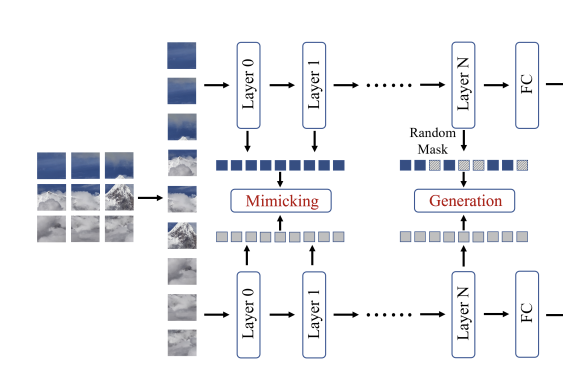
\includegraphics[width=\linewidth]{figures/formula/VITKD.png}
    \caption{Detailed schematic of the ViTKD distillation pipeline applied to the JiT teacher--student pair. \textbf{Top path (mimicking):} hidden-state tensors $\mathbf{F}_i^T$ and $\mathbf{F}_i^S$ from the first two transformer blocks of teacher and student, respectively, are aligned via learned projections $\phi_i$ (plain linear or \texttt{AdaLNAlign}) and compared under an MSE loss $\mathcal{L}_{\text{mimic}}$. \textbf{Bottom path (generation):} the student's final-block features $\mathbf{H}^S$ are linearly projected to $D_T$ dimensions, a random subset of tokens is masked (shown in grey), and a convolutional projector reconstructs the masked positions from spatial context; the reconstruction error against the teacher's final features $\mathbf{H}^T$ defines $\mathcal{L}_{\text{gen}}$. The conditioning vector $\mathbf{c}$ (encoding timestep and class) feeds the \texttt{AdaLNAlign} modulation when timestep conditioning is enabled. All teacher computations are performed without gradient tracking. Dimension annotations: $D_S$ and $D_T$ denote student and teacher embedding dimensions, respectively; $N$ denotes the number of patch tokens.}
    \label{fig:vitkd_pipeline}
\end{figure}

% ============================================================
\section{Attention Map Distillation}
\label{sec:attn_kd}
% ============================================================

A central finding of the recent work by \citet{li2024attentiontransfer} (NeurIPS 2024) challenges the conventional understanding of what pre-training accomplishes in Vision Transformers. The authors demonstrate that the specific feature representations learned during pre-training are not essential to recover its downstream benefits; rather, it is the \emph{attention patterns} — the learned distributions over which tokens attend to which — that constitute the primary carrier of transferable knowledge. They formalise this observation through a method called attention transfer, in which only the post-softmax attention weight matrices of a pretrained teacher ViT are used to supervise a student, while the student is free to develop its own feature representations from scratch. In the attention distillation variant of their framework, the student computes its own attention maps and is trained with an auxiliary cross-entropy loss that encourages those maps to match the teacher's. Despite its simplicity, this approach recovers most of the accuracy gap between training from scratch and full weight fine-tuning on ImageNet-1K classification.

This finding is particularly well-motivated in the pixel-space diffusion setting of JiT. At each denoising timestep $t$, the multi-head self-attention maps of a JiT block directly encode spatial relationships between image patch tokens: which patches attend to which others, reflecting spatial proximity, texture coherence, semantic grouping, and structural layout at the pixel level. Because JiT operates on raw pixel patches rather than abstract latent codes, these attention distributions carry a direct and interpretable correspondence to image content. A teacher model that has been trained to convergence will have developed refined attention routing — grouping semantically related patches, suppressing noisy or uninformative tokens, and resolving long-range spatial dependencies — that a smaller student model has insufficient capacity to discover independently within the same training budget. Supervising the student's attention distributions to approximate those of the teacher therefore transfers a form of relational inductive bias that cannot be conveyed by the output-level flow-matching loss alone.

\subsection*{Attention Map Extraction and Preprocessing}

Attention maps are extracted from the last $K$ transformer blocks of both teacher and student, where $K$ is a hyperparameter (\texttt{num\_attn\_layers}, default $K = 2$). Within each selected block, each of the $H$ attention heads produces a matrix $\mathbf{A} \in \mathbb{R}^{N_{\text{total}} \times N_{\text{total}}}$, where $N_{\text{total}}$ includes both the image patch tokens $N$ and the in-context conditioning tokens appended by JiT's in-context conditioning mechanism. Before the distillation loss is computed, two preprocessing steps are applied. First, the in-context conditioning tokens are stripped, reducing each attention matrix to $\mathbb{R}^{N \times N}$, so that the supervision signal concerns only the spatial routing among image patch tokens and is not confounded by the conditioning tokens. Second, the $H$ per-head maps are averaged across the head dimension to produce a single head-averaged map $\bar{\mathbf{A}} \in \mathbb{R}^{N \times N}$ per block; rows are then renormalised to sum to one, ensuring each row remains a valid probability distribution over the $N$ key positions. This head-averaging strategy is adopted for tractability and consistency: the teacher and student may in general have different numbers of attention heads ($H_T \neq H_S$), and aligning individual heads across architectures introduces an arbitrary correspondence problem. Head-averaging sidesteps this issue cleanly, producing a common spatial routing distribution that is architecture-agnostic.

\subsection*{Distillation Objective: KL Divergence}

Let $\bar{\mathbf{A}}_S^{(\ell)} \in \mathbb{R}^{B \times N \times N}$ and $\bar{\mathbf{A}}_T^{(\ell)} \in \mathbb{R}^{B \times N \times N}$ denote the preprocessed, head-averaged attention maps of the student and teacher at selected layer $\ell \in \{1, \ldots, K\}$, respectively. The attention distillation loss penalises distributional discrepancy between corresponding student and teacher attention maps. Whereas the original attention transfer paper of \cite{li2024attentiontransfer} employs cross-entropy $H(\bar{\mathbf{A}}_T^{(\ell)}, \bar{\mathbf{A}}_S^{(\ell)})$ as the distillation objective, we adopt the Kullback-Leibler (KL) divergence as the primary loss function. This choice is motivated by the fact that the rows of $\bar{\mathbf{A}}$ are proper probability distributions over the $N$ token positions; KL divergence is the canonical information-theoretic measure of how much one distribution diverges from another, and unlike cross-entropy it is invariant to the entropy of the target distribution, making the loss magnitude more interpretable and stable across different noise levels $t$ where the teacher's attention entropy may vary significantly.

For each query token position $n \in \{1, \ldots, N\}$ and each selected layer $\ell$, the KL divergence from the student's distribution to the teacher's is:
%
\begin{equation}
    D_{\mathrm{KL}}\!\left(\bar{\mathbf{A}}_{T,n}^{(\ell)} \,\big\|\, \bar{\mathbf{A}}_{S,n}^{(\ell)}\right)
    = \sum_{n'=1}^{N} \bar{A}_{T,n,n'}^{(\ell)} \log \frac{\bar{A}_{T,n,n'}^{(\ell)}}{\bar{A}_{S,n,n'}^{(\ell)}},
    \label{eq:kl_per_query}
\end{equation}
%
where $\bar{A}_{T,n,n'}^{(\ell)}$ denotes the $(n, n')$ entry of the teacher's head-averaged attention map at layer $\ell$. The full attention distillation loss aggregates over all query tokens, batch samples, and selected layers:
%
\begin{equation}
    \mathcal{L}_{\text{attn}} = \frac{\gamma}{K} \sum_{\ell=1}^{K} \frac{1}{B'} \sum_{b=1}^{B'} \frac{1}{N} \sum_{n=1}^{N} D_{\mathrm{KL}}\!\left(\bar{\mathbf{A}}_{T,b,n}^{(\ell)} \,\big\|\, \bar{\mathbf{A}}_{S,b,n}^{(\ell)}\right),
    \label{eq:loss_attn}
\end{equation}
%
where $\gamma$ is a scalar loss weight (\texttt{gamma\_attn}, default $\gamma = 10^{-4}$), $B' \leq B$ is the number of samples in the batch that pass the timestep gate (described below), and the division by $K$ normalises the loss magnitude to be independent of the number of supervised layers. A numerical stability offset $\varepsilon = 10^{-8}$ is added to all attention weights before computing the logarithm, followed by a renormalisation pass to ensure strict distributional validity. We additionally investigate a \textbf{symmetric} variant of the loss, defined as $\frac{1}{2}\left[D_{\mathrm{KL}}(\bar{\mathbf{A}}_T \| \bar{\mathbf{A}}_S) + D_{\mathrm{KL}}(\bar{\mathbf{A}}_S \| \bar{\mathbf{A}}_T)\right]$, which penalises divergence in both directions and may be preferable when the student and teacher attention distributions overlap substantially. The asymmetric variant (default) enforces a one-directional pressure pushing the student toward the teacher without penalising the student for distributing probability mass differently in regions the teacher ignores.

\subsection*{Timestep Gating}

A critical consideration specific to the diffusion setting is that at very low noise levels — concretely, for $t \leq t_{\min}$ (default $t_{\min} = 0.1$) — the noisy input $\mathbf{z} = t\mathbf{x} + (1-t)\mathbf{e}$ is dominated by Gaussian noise and carries negligible image content. In this regime, the attention maps of both teacher and student tend toward near-uniform distributions, as no meaningful spatial structure is recoverable from the near-pure-noise input. Supervising the student to match the teacher's near-uniform attention at these timesteps would inject gradient noise rather than useful signal, potentially destabilising training. Accordingly, any sample $b$ in the batch for which $t_b \leq t_{\min}$ is excluded from $\mathcal{L}_{\text{attn}}$: the gated batch size $B'$ in Equation~\eqref{eq:loss_attn} counts only those samples for which $t_b > t_{\min}$. If all samples in a batch fall below this threshold, the attention loss evaluates to zero for that step. The full set of hyperparameters governing the attention distillation loss is summarised in Table~\ref{tab:attn_hyperparams}.

\begin{table}[ht]
    \centering
    \caption{Hyperparameters of the attention map distillation loss. Default values reflect those used in the primary experimental configuration; ablation over selected hyperparameters is reported in Chapter~\ref{chap:experiments}.}
    \label{tab:attn_hyperparams}
    \begin{tabular}{lccl}
        \toprule
        \textbf{Hyperparameter} & \textbf{Symbol} & \textbf{Default} & \textbf{Role} \\
        \midrule
        Attention loss weight    & $\gamma$       & $10^{-4}$         & Overall scale of $\mathcal{L}_{\text{attn}}$ \\
        Number of supervised layers & $K$         & $2$               & Last $K$ blocks used for supervision \\
        Timestep gate threshold  & $t_{\min}$    & $0.1$             & Excludes near-noise samples \\
        Numerical stability      & $\varepsilon$ & $10^{-8}$         & Added before log to prevent $\log(0)$ \\
        Symmetric KL             & ---           & enabled           & Uses $\frac{1}{2}(\mathrm{KL}_{T\to S} + \mathrm{KL}_{S\to T})$ \\
        \bottomrule
    \end{tabular}
\end{table}

\begin{figure}[ht]
    \centering
    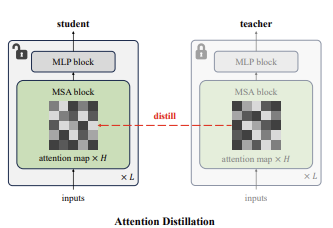
\includegraphics[width=\linewidth]{figures/formula/attn-d.png}
    \caption{Illustration of the attention map distillation procedure. From each of the last $K$ transformer blocks, the $H$ per-head attention matrices are extracted from both teacher (frozen) and student (trainable), averaged across heads, and stripped of in-context conditioning tokens to yield spatial routing distributions $\bar{\mathbf{A}}_T^{(\ell)}, \bar{\mathbf{A}}_S^{(\ell)} \in \mathbb{R}^{N \times N}$. Samples with $t \leq t_{\min}$ are excluded (greyed out). KL divergence is computed between the resulting distributions and aggregated across layers and tokens to form $\mathcal{L}_{\text{attn}}$. No learnable parameters are introduced by this component; the student's attention maps are computed by its own multi-head self-attention mechanism.}
    \label{fig:attn_kd_pipeline}
\end{figure}

The attention distillation component introduces no learnable parameters: the student's attention maps are produced by its own query--key dot-product mechanism, and no projection or alignment layer is required because both teacher and student produce head-averaged maps of the same spatial dimension $N \times N$, regardless of their respective embedding dimensions or head counts. This makes the attention loss computationally inexpensive relative to the ViTKD feature distillation, as it requires only the collection of attention weight matrices during the student and teacher forward passes — operations that are already performed internally and need only be returned rather than discarded.


% ============================================================
\section{Weight Selection as Complementary Initialisation}
\label{sec:weight_selection}
% ============================================================

The two distillation methods described in Sections~\ref{sec:vitkd} and~\ref{sec:attn_kd} are \emph{online} training objectives: they are evaluated and differentiated at every gradient step throughout the entire training run. Weight selection \cite{xu2024initializing}, by contrast, is an \emph{offline} initialisation strategy that is applied once, before any gradient update, and whose effect is therefore mediated entirely through the quality of the student's starting point on the loss landscape. It is nonetheless a meaningful component of the framework, as the starting point from which distillation training begins can substantially influence both the convergence speed and the quality of the eventual solution.

\subsection*{Method}

\cite{xu2024initializing} (ICLR 2024, Spotlight) introduce weight selection as a general technique for initialising a smaller model by extracting a structured subset of weights from a larger, pretrained counterpart. The key observation motivating the method is that, in the large-model era, pretrained weights encode learned representations, inductive biases, and optimised parameter configurations that took substantial compute to acquire. Discarding this information entirely in favour of random initialisation — as is standard practice when training a smaller model from scratch — is unnecessarily wasteful. Weight selection proposes instead to \emph{inherit} a portion of the teacher's learned knowledge directly through the initialisation of the student's parameters, at zero additional training cost.

The initialisation procedure operates parameter-tensor by parameter-tensor. For each learnable parameter key $k$ present in both teacher and student state dictionaries, the following cases are handled. If the teacher and student tensors at key $k$ have identical shapes, the teacher tensor is copied directly into the student. If the teacher tensor is strictly larger than the student tensor in one or more dimensions — which is the generic case when the student has fewer hidden units or fewer layers — a \emph{uniform element selection} is applied: for each dimension $d$ in which the shapes differ, a set of $s_d$ indices is drawn at uniform spacing from the teacher's $t_d$ entries, where $s_d$ and $t_d$ are the student and teacher sizes along dimension $d$, respectively. When $t_d$ is divisible by $s_d$, a regular stride of $t_d / s_d$ is used; otherwise, indices are computed via evenly-spaced linspace rounding. This selection is applied sequentially across all differing dimensions, yielding a student-shaped sub-tensor drawn from the teacher. Parameters for which the teacher tensor is smaller than the student tensor in any dimension, or whose key is absent from the teacher's state dictionary, are left at their default random initialisation.

\subsection*{Application to JiT and Handling of Architectural Mismatches}

Applying weight selection to the JiT model family requires careful handling of several architecture-specific considerations. The primary cases encountered in our experimental pairs are summarised as follows.

\paragraph{Hidden dimension reduction.} In the CIFAR-10 setting, the teacher is JiT-S/2 with hidden dimension $D_T = 512$ and the student is JiT-T/2 with $D_S = 384$. All weight matrices of the form $\mathbf{W} \in \mathbb{R}^{D_T \times D_T}$ — including query, key, value, and projection weight matrices in every attention block, as well as FFN weight matrices — are reduced to $\mathbb{R}^{D_S \times D_S}$ by uniform selection along both dimensions. In the ImageNet setting, the teacher is JiT-B/16 with $D_T = 768$ and the student is JiT-S/16 with $D_S = 384$; the same procedure applies.

\paragraph{Depth reduction.} In the CIFAR-10 pair, the teacher has 10 transformer blocks and the student has 6. Since the student has fewer layers, the selected layers must be chosen from the teacher's depth. In our implementation, the student's layers are matched to the teacher's by a uniform stride across the teacher's block indices, preserving early and late layers which encode respectively the low-level denoising patterns and the high-level velocity prediction structure.

\paragraph{Non-learnable and regenerated parameters.} Positional embedding buffers (\texttt{pos\_embed}), rotary embedding frequency tensors (\texttt{freqs\_cos}, \texttt{freqs\_sin}), and similar deterministic buffers are excluded from weight selection and recomputed from the student's own configuration. These quantities depend on the model's spatial resolution and sequence length and cannot be meaningfully inherited from the teacher.

\paragraph{Class embedding remapping.} When the teacher was trained on a dataset with a different number of classes than the student's target (e.g., a teacher pretrained on ImageNet-1K being adapted to CIFAR-10), the class embedding table $\mathbf{E}_y \in \mathbb{R}^{(C+1) \times D}$ — where $C$ is the number of classes and the extra row corresponds to the unconditional null class — has incompatible first dimensions. In this case, the class embeddings are excluded from weight selection and re-initialised randomly in the student. This is an expected and handled edge case in our codebase.

\subsection*{Role Within the Framework}

Weight selection is complementary to the ViTKD and attention distillation losses in a precise sense: it does not introduce any additional loss term, does not modify the training loop, and does not impose any computational overhead during training. Its benefit is expressed entirely through the starting configuration of the student's parameters. A student initialised via weight selection begins its training in a region of parameter space that is structurally similar to a converged teacher — its attention heads already encode meaningful queries and keys, its MLP weights already perform useful feature transformations, and its adaLN modulation layers are already calibrated to reasonable scale and shift ranges. This informed starting point means that the ViTKD and attention distillation losses, which provide supervision from the teacher's internal representations throughout training, operate on a student that is already in approximate alignment with the teacher from step zero, rather than having to first correct the large initial mismatch that would arise from random initialisation. Empirically, this is expected to translate into faster convergence and potentially higher final performance, as the distillation losses can focus on refining rather than bootstrapping the student's representations. The combination of weight selection initialisation with online distillation training is accordingly the recommended default configuration of the proposed framework.

\begin{figure}[ht]
    \centering
    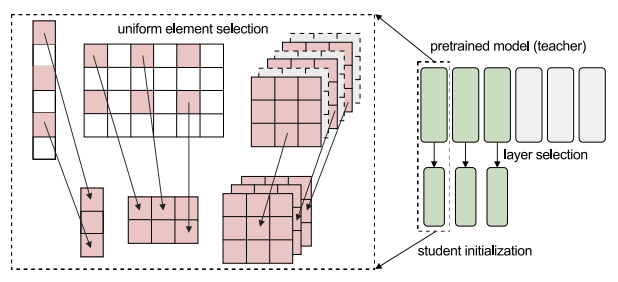
\includegraphics[width=0.85\linewidth]{figures/formula/weight-selection.png}
    \caption{Illustration of the weight selection initialisation procedure for the JiT-S/2 $\to$ JiT-T/2 pair ($D_T = 512$, $D_S = 384$, teacher depth 10, student depth 6). \textbf{Left:} for each weight matrix, a structured subset of rows and columns is selected at uniform spacing from the teacher tensor (shown in orange), yielding a student-sized initialisation (shown in blue). \textbf{Right:} layer correspondence for the depth reduction case; the student's 6 blocks are matched to 6 of the teacher's 10 blocks at uniform stride, preserving both early and late layers.}
    \label{fig:weight_selection}
\end{figure}


% ============================================================
\section{Unified Training Objective}
\label{sec:unified_objective}
% ============================================================

The three components described in the preceding sections are integrated into a single training procedure. Weight selection provides a one-time initialisation of the student's parameters from the teacher's pretrained weights before training commences. During each subsequent training step, the student is optimised under a combined loss that aggregates the base denoising objective with the two distillation losses:
%
\begin{equation}
    \mathcal{L}_{\text{total}} = \mathcal{L}_{\text{flow}} + \mathcal{L}_{\text{ViTKD}} + \mathcal{L}_{\text{attn}},
    \label{eq:loss_total}
\end{equation}
%
where each term serves a distinct supervisory role. The flow-matching denoising loss $\mathcal{L}_{\text{flow}}$ ensures that the student remains a well-formed generative model, trained to predict the velocity field of the probability flow ODE for the data distribution. For a batch of clean images $\mathbf{x}$ and class labels $y$, with noise $\mathbf{e} \sim \mathcal{N}(\mathbf{0}, \sigma^2 \mathbf{I})$ and timestep $t$ sampled from a log-normal distribution mapped through the sigmoid function, the noisy input is $\mathbf{z} = t\mathbf{x} + (1-t)\mathbf{e}$ and the target velocity is $\mathbf{v} = (\mathbf{x} - \mathbf{z}) / (1 - t)$. The denoising loss is:
%
\begin{equation}
    \mathcal{L}_{\text{flow}} = \mathbb{E}_{t, \mathbf{x}, \mathbf{e}, y}\!\left[ \left\| \mathbf{v}_\theta(\mathbf{z}, t, y) - \mathbf{v} \right\|_2^2 \right],
    \label{eq:loss_flow}
\end{equation}
%
where $\mathbf{v}_\theta$ denotes the student's velocity prediction. The ViTKD loss $\mathcal{L}_{\text{ViTKD}} = \mathcal{L}_{\text{mimic}} + \mathcal{L}_{\text{gen}}$ (Equation~\eqref{eq:loss_vitkd}) transfers intermediate feature map knowledge from the teacher's shallow and deep transformer blocks. The attention distillation loss $\mathcal{L}_{\text{attn}}$ (Equation~\eqref{eq:loss_attn}) transfers the teacher's learned spatial routing patterns. The relative magnitudes of the three loss components are governed by the hyperparameters $\alpha$, $\beta$, and $\gamma$; in practice, $\mathcal{L}_{\text{flow}}$ is of order one, while $\mathcal{L}_{\text{ViTKD}}$ and $\mathcal{L}_{\text{attn}}$ are scaled to be approximately one to two orders of magnitude smaller, ensuring that the distillation signal acts as a regulariser on the student's internal representations without displacing the primary generative objective.

The teacher's weights are held frozen for the entirety of training. Concretely, no gradients are propagated through the teacher's parameters at any point; all teacher forward passes are executed under \texttt{torch.no\_grad()}. The only parameters updated by backpropagation are those of the student network and the ViTKD alignment layers ($\{\mathbf{W}_i\}$, $\mathbf{W}_{\text{deep}}$, $\boldsymbol{\mu}$, and the convolutional projector weights). The attention distillation component introduces no additional learnable parameters. Following each gradient update, an exponential moving average (EMA) of the student's parameters is maintained — independently of the teacher — and used for all generation and evaluation passes. Algorithm~\ref{alg:distill_training} provides a concise summary of one complete training step.

\begin{algorithm}[ht]
\caption{One Training Step of the Distillation Framework}
\label{alg:distill_training}
\begin{algorithmic}[1]
    \Require Clean images $\mathbf{x}$, class labels $y$; frozen teacher $f_T$; student $f_S$ (trainable); ViTKD loss module $\mathcal{L}_{\text{ViTKD}}$; attention KD loss module $\mathcal{L}_{\text{attn}}$
    \State Sample $t \sim \sigma({\mathcal{N}(\mu_P, \sigma_P^2)})$, $\mathbf{e} \sim \mathcal{N}(\mathbf{0}, \sigma_{\text{noise}}^2\mathbf{I})$
    \State $\mathbf{z} \leftarrow t\mathbf{x} + (1-t)\mathbf{e}$ \Comment{Construct noisy image}
    \State $\mathbf{v} \leftarrow (\mathbf{x} - \mathbf{z}) / (1-t)$ \Comment{Target velocity}
    \State $\hat{\mathbf{v}}_S,\, \mathbf{F}_S,\, \mathbf{A}_S \leftarrow f_S(\mathbf{z}, t, y)$ \Comment{Student forward pass; collect features and attention maps}
    \State $\mathcal{L}_{\text{flow}} \leftarrow \|\hat{\mathbf{v}}_S - \mathbf{v}\|_2^2$
    \State \textbf{with} \texttt{no\_grad():}
    \State \quad $\mathbf{F}_T,\, \mathbf{A}_T \leftarrow f_T(\mathbf{z}, t, y)$ \Comment{Teacher forward pass; no gradient}
    \State $\mathcal{L}_{\text{ViTKD}} \leftarrow \mathcal{L}_{\text{mimic}}(\mathbf{F}_S^{\text{low}}, \mathbf{F}_T^{\text{low}}) + \mathcal{L}_{\text{gen}}(\mathbf{F}_S^{\text{high}}, \mathbf{F}_T^{\text{high}})$
    \State $\mathcal{L}_{\text{attn}} \leftarrow \mathcal{L}_{\text{attn}}(\mathbf{A}_S, \mathbf{A}_T, t)$ \Comment{Gated by $t > t_{\min}$}
    \State $\mathcal{L}_{\text{total}} \leftarrow \mathcal{L}_{\text{flow}} + \mathcal{L}_{\text{ViTKD}} + \mathcal{L}_{\text{attn}}$
    \State $\theta_S \leftarrow \theta_S - \eta \nabla_{\theta_S} \mathcal{L}_{\text{total}}$ \Comment{Update student and alignment layers only}
    \State Update student EMA parameters \Comment{Teacher EMA not updated}
\end{algorithmic}
\end{algorithm}

The modular structure of the framework offers flexibility in ablation: any subset of the three components can be enabled or disabled independently. The ViTKD and attention distillation losses can each be toggled individually; weight selection can be replaced by standard random initialization; and within ViTKD, the generation loss can be ablated via the \texttt{mimic\_only} flag. This modularity is exploited systematically in the experimental evaluation of Chapter~\ref{chap:experiments}, where the contribution of each component is isolated and quantified.
    % ============================================================
%  CHAPTER: Experiments and Results
%  Thesis: Knowledge Distillation in Diffusion Models for Image Generation
%  NTUA School of Electrical and Computer Engineering
% ============================================================

\chapter{Experiments and Results}
\label{chap:experiments}

This chapter presents the empirical evaluation of the distillation framework
described in Chapter~\ref{chap:framework}. The objective of the
experiments is to validate the central claim of the thesis: that,
for the same student model architecture and inference cost, distillation
training produces a strictly superior generative model compared to training
the student from scratch. The chapter is structured as follows.
Section~\ref{sec:setup} specifies the datasets, model configurations, training
protocol, computational resources, and evaluation methodology.
Section~\ref{sec:main_results} reports the results of the experiments. Section~\ref{sec:disc_limits} discusses the results and acknowledges limitations.

% ============================================================
\section{Experimental Setup}
\label{sec:setup}
% ============================================================

\subsection{Datasets and Preprocessing}
\label{subsec:datasets}

The main dataset used is \textbf{Imagenette} which contains 10{,}000 training images evenly distributed across 10 classes. The images are resized to $256 \times 256$ pixels for all experiments. Images preprocessing consist of: a centre-crop that is applied using the implementation of
\cite{dhariwal2021diffusion} to preserve the principal content of each image,
followed by random horizontal flipping as the sole data augmentation strategy.
Pixel values are normalised from the range $[0, 255]$ to $[-1, 1]$ prior to
being passed to the model, and class labels are used as conditioning
information throughout.

% ============================================================
\subsection{Model Configurations and Baselines}
\label{subsec:models}

All experiments are conducted using the Just-image Transformer (JiT)
architecture~\cite{li2025jit}, a minimalist pixel-space diffusion model based
on a Vision Transformer backbone~\cite{dosovitskiy2020vit} trained with a
flow-matching objective. Two model variants are considered, their architectural specifications are
summarized in Table~\ref{tab:model_configs}.

\begin{table}[ht]
    \centering
    \caption{Architectural specifications of the two JiT model variants used
    in this work. $L$ denotes the number of transformer blocks, $D$ the hidden
    dimension, $H$ the number of attention heads, $P$ the patch size in pixels,
    $C$ the in-context conditioning token length, and \#Params the total
    parameter count.}
    \label{tab:model_configs}
    \begin{tabular}{lcccccc}
        \toprule
        Model & $L$ & $D$ & $H$ & $P$ & $C$ & \#Params \\
        \midrule
        JiT-S/16 & 12 & 384 &  6 & 16 & 32 & 33.3M \\
        JiT-B/16 & 12 & 768 & 12 & 16 & 32 & 131M \\
        \bottomrule
    \end{tabular}
\end{table}

The JiT-S/16 student is distilled from a pretrained
JiT-B/16 teacher on ImageNet-1K at $256 \times 256$ resolution. The primary baseline in all comparisons is the
corresponding student architecture trained from scratch under an identical
training budget and optimization configuration, with no access to teacher
supervision.

% ============================================================
\subsection{Training Protocol and Hyperparameters}
\label{subsec:training}

All models are trained with the AdamW optimiser~\cite{loshchilov2019decoupled}
with momentum coefficients $\beta_1 = 0.9$ and $\beta_2 = 0.95$ and no weight
decay. The learning rate is set according to the linear scaling rule,
$\eta = \eta_\text{base} \times B_\text{eff} / 256$, with a base learning
rate of $\eta_\text{base} = 5 \times 10^{-5}$ and a warmup period of 5 epochs.
Two EMA tracks of the student parameters are maintained throughout training,
with decay constants $\mu_1 = 0.9999$ and $\mu_2 = 0.9996$; sampling at
evaluation time uses the first EMA track exclusively. Training is performed
in \texttt{bfloat16} mixed precision. The complete set of training
hyperparameters is provided in
Table~\ref{tab:training_hparams}.

\begin{table}[ht]
    \centering
    \caption{Training hyperparameters for the experimental setting.}
    \label{tab:training_hparams}
    \begin{tabular}{lc}
        \toprule
        Hyperparameter & Imagenette (JiT-S/16) \\
        \midrule
        Batch size (per GPU)           & 128 \\
        Effective batch size           & 128 \\
        Base LR ($\eta_\text{base}$)   & $5 \times 10^{-5}$ \\
        LR schedule                    & constant      \\
        Warmup epochs                  & 5             \\
        EMA decay $\mu_1$              & 0.9999        \\
        EMA decay $\mu_2$              & 0.9996        \\
        Weight decay                   & 0.0           \\
        Precision                      & BF16          \\
        $\alpha_\text{ViTKD}$          & $3\times10^{-5}$ \\
        $\beta_\text{ViTKD}$           & $3\times10^{-6}$ \\
        $\lambda_\text{ViTKD}$         & 0.5           \\
        $\gamma_\text{attn}$           & $1\times10^{-4}$ \\
        $K$ (attn layers)              & 2             \\
        $t_{\min}$ (attn gate)         & 0.1           \\
        \bottomrule
    \end{tabular}
\end{table}


% ============================================================
\subsection{Computational Resources}
\label{subsec:compute}

The small-scale experiments on CIFAR-10 were conducted on the Kaggle
computational platform, utilising two NVIDIA Tesla T4 GPUs (16\,GB VRAM each)
in a distributed data-parallel configuration. The experiments were conducted on Google Colab Pro, utilising a single NVIDIA A100
GPU (40\,GB VRAM).

% ============================================================
\subsection{Evaluation Protocol}
\label{subsec:eval}

Generative quality is assessed using two standard metrics: the
Fréchet Inception Distance (FID)~\cite{heusel2017gans} and the Inception Score
(IS)~\cite{salimans2016improved}. FID and IS are computed over 50{,}000
generated images to ensure statistical reliability;
All metrics are evaluated using the \texttt{torch-fidelity} library. At
inference time, sampling is performed with the Heun second-order ODE solver
with 50 function evaluations (NFE), and classifier-free
guidance~\cite{ho2022classifier} is applied with a fixed scale and interval
per setting. All evaluations use the first EMA track of the student model.






















































% ============================================================
%  SECTION 7.2 — Main Results
%  Thesis: Knowledge Distillation in Diffusion Models for Image Generation
%  NTUA School of Electrical and Computer Engineering
% ============================================================
%
%  REQUIRED PACKAGES (add to your preamble if not already present):
%
%    \usepackage{pgfplots}
%    \pgfplotsset{compat=1.18}
%    \usepackage{subcaption}   % for subfigure environments
%    \usepackage{booktabs}     % for \toprule, \midrule, \bottomrule in tables
%    \usepackage{xcolor}       % for custom color definitions
%
% ============================================================
%
%  COLOR DEFINITIONS
%  -----------------
%  Define the two bar colors here once; every figure below references
%  them by name, so changing a single line updates all plots globally.
%
%  Available color models in xcolor:
%    RGB  (0-255 each channel) :  \definecolor{name}{RGB}{r,g,b}
%    rgb  (0.0-1.0 each channel):  \definecolor{name}{rgb}{r,g,b}
%    HTML (hex string)         :  \definecolor{name}{HTML}{RRGGBB}
%    named colors (predefined) :  blue, red, gray, teal, olive, ...
%
\definecolor{colorBaseline}{RGB}{150, 150, 150}   % neutral gray  — baseline bar
\definecolor{colorExperiment}{RGB}{0, 84, 159}    % NTUA deep blue — experiment bar

% ============================================================
%
%  PGFPLOTS GLOBAL STYLE
%  ---------------------
%  Setting a global style here avoids repeating the same keys in
%  every axis environment. Override any key locally inside a specific
%  axis if needed.
%
\pgfplotsset{
    resultbar/.style={
        ybar,                        % vertical bar chart
        bar width     = 18pt,        % width of each bar in points; increase for fatter bars
        width         = 0.44\linewidth, % total plot width; adjust with \linewidth fraction
        height        = 5.5cm,       % total plot height; adjust in cm or pt
        enlarge x limits = 0.55,     % extra horizontal padding around bars (0–1 scale)
        symbolic x coords = {Baseline, Experiment}, % x-tick labels
        xtick         = data,
        ymin          = 0,           % y-axis lower bound; set explicitly to avoid clipping
        % ymax        = 100,         % uncomment and set to fix the y-axis upper bound
        ymajorgrids   = true,        % horizontal grid lines; set to false to remove
        grid style    = {dashed, gray!40},
        tick align    = outside,
        xtick style   = {draw=none}, % hide the small tick marks on the x-axis
        every axis/.append style = {font=\small},
        nodes near coords,           % print the numeric value on top of each bar
        % -------------------------------------------------------
        % To DISABLE numeric labels on top of bars, comment out
        % the "nodes near coords" line above and uncomment below:
        % nodes near coords = {},
        % -------------------------------------------------------
        nodes near coords align = {vertical},
        every node near coord/.append style = {font=\footnotesize},
        legend style = {
            at        = {(0.5, -0.22)}, % legend position: below the plot
            anchor    = north,
            legend columns = 2,        % number of columns in the legend
            font      = \footnotesize,
        },
    },
}

% ============================================================
\section{Main Results}
\label{sec:main_results}
% ============================================================

This section presents the quantitative results of the eight experimental
configurations evaluated on Imagenette at $256 \times 256$ resolution.
All results are obtained using the JiT-S/16 student architecture and are
reported in terms of Fréchet Inception Distance (FID; lower is better)
and Inception Score (IS; higher is better), computed over 50{,}000
generated images as described in Section~\ref{subsec:eval}. Each
subsection below follows the same structure: a brief description of the
experimental configuration, a figure containing side-by-side bar plots
for FID and IS, and a concise numerical interpretation of the outcome.
In all comparison figures, the left bar corresponds to the no-distillation
baseline (Experiment~1) and the right bar to the configuration under
examination, so that the magnitude of any improvement or regression is
immediately apparent.

% ============================================================
\subsection{Experiment 1: Baseline JiT-S/16 without Distillation}
\label{subsec:exp1}
% ============================================================

The first experiment establishes the performance floor of the JiT-S/16
student model when trained from scratch under the standard flow-matching
objective, with no teacher supervision of any kind. This configuration
serves as the reference point against which all subsequent distillation
experiments are evaluated. The model is trained with the hyperparameters
specified in Table~\ref{tab:training_hparams} and evaluated using the
first EMA track of the student weights.

\begin{figure}[ht]
    \centering
    %
    % ----- FID subplot (lower is better) -----
    \begin{subfigure}[b]{0.44\linewidth}
        \centering
        \begin{tikzpicture}
            \begin{axis}[
                resultbar,
                ylabel       = {FID $(\downarrow)$},  % axis label; \downarrow signals lower=better
                title        = {FID},
            ]
            \addplot[fill=colorBaseline, draw=colorBaseline!70!black]
                coordinates {(Baseline, 99.99)};  % TODO: replace 99.99 with actual FID value
            \legend{Baseline}
            \end{axis}
        \end{tikzpicture}
    \end{subfigure}
    \hfill
    % ----- IS subplot (higher is better) -----
    \begin{subfigure}[b]{0.44\linewidth}
        \centering
        \begin{tikzpicture}
            \begin{axis}[
                resultbar,
                ylabel       = {IS $(\uparrow)$},     % axis label; \uparrow signals higher=better
                title        = {Inception Score},
            ]
            \addplot[fill=colorBaseline, draw=colorBaseline!70!black]
                coordinates {(Baseline, 9.99)};   % TODO: replace 9.99 with actual IS value
            \legend{Baseline}
            \end{axis}
        \end{tikzpicture}
    \end{subfigure}
    %
    \caption{Experiment~1 — Baseline JiT-S/16 trained from scratch without
    any distillation. FID (left; lower is better) and IS (right; higher is
    better) serve as the reference metrics for all subsequent experiments.}
    \label{fig:exp1_results}
\end{figure}

The baseline JiT-S/16, trained without any distillation, achieves an FID
of \textbf{XX.XX} and an IS of \textbf{XX.XX}.   % TODO: fill in values
These figures represent the upper bound on FID and the lower bound on IS
that the distillation experiments are expected to improve upon.

% ============================================================
\subsection{Experiment 2: JiT-S/16 with ViTKD Mimic Distillation}
\label{subsec:exp2}
% ============================================================

The second experiment introduces the mimic component of the ViTKD
framework~\cite{yang2022vitkd} as the sole distillation signal. The mimic
loss encourages the student's intermediate feature maps to match those of
the frozen teacher at selected transformer blocks, using a lightweight
linear projection to bridge the hidden-dimension mismatch between the two
architectures. No projector loss is applied in this configuration.

\begin{figure}[ht]
    \centering
    %
    \begin{subfigure}[b]{0.44\linewidth}
        \centering
        \begin{tikzpicture}
            \begin{axis}[
                resultbar,
                ylabel = {FID $(\downarrow)$},
                title  = {FID},
            ]
            \addplot[fill=colorBaseline, draw=colorBaseline!70!black]
                coordinates {(Baseline, 99.99)};      % TODO: baseline FID
            \addplot[fill=colorExperiment, draw=colorExperiment!70!black]
                coordinates {(Experiment, 99.99)};    % TODO: Exp 2 FID
            \legend{Baseline, Mimic only}
            \end{axis}
        \end{tikzpicture}
    \end{subfigure}
    \hfill
    \begin{subfigure}[b]{0.44\linewidth}
        \centering
        \begin{tikzpicture}
            \begin{axis}[
                resultbar,
                ylabel = {IS $(\uparrow)$},
                title  = {Inception Score},
            ]
            \addplot[fill=colorBaseline, draw=colorBaseline!70!black]
                coordinates {(Baseline, 9.99)};       % TODO: baseline IS
            \addplot[fill=colorExperiment, draw=colorExperiment!70!black]
                coordinates {(Experiment, 9.99)};     % TODO: Exp 2 IS
            \legend{Baseline, Mimic only}
            \end{axis}
        \end{tikzpicture}
    \end{subfigure}
    %
    \caption{Experiment~2 — JiT-S/16 trained with the ViTKD mimic loss
    only, compared against the no-distillation baseline. FID (left; lower
    is better) and IS (right; higher is better).}
    \label{fig:exp2_results}
\end{figure}

Applying mimic distillation alone yields an FID of \textbf{XX.XX} and an
IS of \textbf{XX.XX}, compared to the baseline FID of \textbf{XX.XX} and  % TODO: fill in values
IS of \textbf{XX.XX}. This corresponds to a [improvement/regression] of
approximately \textbf{XX.XX} FID points and \textbf{XX.XX} IS points
relative to the baseline.

% ============================================================
\subsection{Experiment 3: JiT-S/16 with Full ViTKD Distillation}
\label{subsec:exp3}
% ============================================================

Experiment~3 extends the previous configuration by adding the projector
loss to the mimic loss, thereby activating the full ViTKD objective. The
projector loss operates on a deeper layer of the student's feature
hierarchy and introduces a more structured alignment target between student
and teacher representations.

\begin{figure}[ht]
    \centering
    %
    \begin{subfigure}[b]{0.44\linewidth}
        \centering
        \begin{tikzpicture}
            \begin{axis}[
                resultbar,
                ylabel = {FID $(\downarrow)$},
                title  = {FID},
            ]
            \addplot[fill=colorBaseline, draw=colorBaseline!70!black]
                coordinates {(Baseline, 99.99)};      % TODO: baseline FID
            \addplot[fill=colorExperiment, draw=colorExperiment!70!black]
                coordinates {(Experiment, 99.99)};    % TODO: Exp 3 FID
            \legend{Baseline, Full ViTKD}
            \end{axis}
        \end{tikzpicture}
    \end{subfigure}
    \hfill
    \begin{subfigure}[b]{0.44\linewidth}
        \centering
        \begin{tikzpicture}
            \begin{axis}[
                resultbar,
                ylabel = {IS $(\uparrow)$},
                title  = {Inception Score},
            ]
            \addplot[fill=colorBaseline, draw=colorBaseline!70!black]
                coordinates {(Baseline, 9.99)};       % TODO: baseline IS
            \addplot[fill=colorExperiment, draw=colorExperiment!70!black]
                coordinates {(Experiment, 9.99)};     % TODO: Exp 3 IS
            \legend{Baseline, Full ViTKD}
            \end{axis}
        \end{tikzpicture}
    \end{subfigure}
    %
    \caption{Experiment~3 — JiT-S/16 trained with the full ViTKD objective
    (mimic and projector losses), compared against the no-distillation
    baseline. FID (left; lower is better) and IS (right; higher is better).}
    \label{fig:exp3_results}
\end{figure}

The full ViTKD configuration yields an FID of \textbf{XX.XX} and an IS of
\textbf{XX.XX}. Relative to Experiment~2 (mimic only; FID \textbf{XX.XX},  % TODO: fill in values
IS \textbf{XX.XX}), the addition of the projector loss results in a
[improvement/regression], suggesting that the projector component
[adds complementary signal / introduces conflicting gradients] in this
setting. This observation motivates the adoption of the mimic-only
configuration as the feature distillation component in subsequent
combined experiments.

% ============================================================
\subsection{Experiment 4: JiT-S/16 with ViTKD Mimic and SNR-Weighted Loss}
\label{subsec:exp4}
% ============================================================

Experiment~4 augments the mimic-only distillation of Experiment~2 with
an SNR-based loss weighting scheme. Specifically, a min-SNR-$\gamma$
reweighting~\cite{hang2023efficient} is applied to both the flow-matching
and distillation objectives with $\gamma = 0.5$, clamping the effective
loss weight at each timestep $t$ to prevent high-noise timesteps from
dominating the gradient signal. The mimic loss is retained in preference
to the full ViTKD objective on the basis that Experiment~2 demonstrated
superior performance to Experiment~3.

\begin{figure}[ht]
    \centering
    %
    \begin{subfigure}[b]{0.44\linewidth}
        \centering
        \begin{tikzpicture}
            \begin{axis}[
                resultbar,
                ylabel = {FID $(\downarrow)$},
                title  = {FID},
            ]
            \addplot[fill=colorBaseline, draw=colorBaseline!70!black]
                coordinates {(Baseline, 99.99)};      % TODO: baseline FID
            \addplot[fill=colorExperiment, draw=colorExperiment!70!black]
                coordinates {(Experiment, 99.99)};    % TODO: Exp 4 FID
            \legend{Baseline, Mimic + SNR-$\gamma$}
            \end{axis}
        \end{tikzpicture}
    \end{subfigure}
    \hfill
    \begin{subfigure}[b]{0.44\linewidth}
        \centering
        \begin{tikzpicture}
            \begin{axis}[
                resultbar,
                ylabel = {IS $(\uparrow)$},
                title  = {Inception Score},
            ]
            \addplot[fill=colorBaseline, draw=colorBaseline!70!black]
                coordinates {(Baseline, 9.99)};       % TODO: baseline IS
            \addplot[fill=colorExperiment, draw=colorExperiment!70!black]
                coordinates {(Experiment, 9.99)};     % TODO: Exp 4 IS
            \legend{Baseline, Mimic + SNR-$\gamma$}
            \end{axis}
        \end{tikzpicture}
    \end{subfigure}
    %
    \caption{Experiment~4 — JiT-S/16 trained with the ViTKD mimic loss
    and min-SNR-$\gamma$ reweighting ($\gamma = 0.5$), compared against
    the no-distillation baseline. FID (left; lower is better) and IS
    (right; higher is better).}
    \label{fig:exp4_results}
\end{figure}

With SNR reweighting enabled, the model achieves an FID of \textbf{XX.XX}
and an IS of \textbf{XX.XX}. Relative to the mimic-only baseline of      % TODO: fill in values
Experiment~2 (FID \textbf{XX.XX}, IS \textbf{XX.XX}), this represents a
[improvement/regression], indicating that timestep-aware loss weighting
[does / does not] provide a meaningful complementary benefit to feature
map distillation in this setting.

% ============================================================
\subsection{Experiment 5: JiT-S/16 with Attention Map Distillation}
\label{subsec:exp5}
% ============================================================

Experiment~5 investigates a qualitatively different distillation signal:
rather than aligning intermediate feature maps, the attention distillation
loss encourages the student to reproduce the teacher's post-softmax
self-attention weight matrices in the final $K = 2$ transformer blocks.
No ViTKD loss of any kind is applied in this configuration, isolating the
contribution of structural attention transfer.

\begin{figure}[ht]
    \centering
    %
    \begin{subfigure}[b]{0.44\linewidth}
        \centering
        \begin{tikzpicture}
            \begin{axis}[
                resultbar,
                ylabel = {FID $(\downarrow)$},
                title  = {FID},
            ]
            \addplot[fill=colorBaseline, draw=colorBaseline!70!black]
                coordinates {(Baseline, 99.99)};      % TODO: baseline FID
            \addplot[fill=colorExperiment, draw=colorExperiment!70!black]
                coordinates {(Experiment, 99.99)};    % TODO: Exp 5 FID
            \legend{Baseline, Attention KD}
            \end{axis}
        \end{tikzpicture}
    \end{subfigure}
    \hfill
    \begin{subfigure}[b]{0.44\linewidth}
        \centering
        \begin{tikzpicture}
            \begin{axis}[
                resultbar,
                ylabel = {IS $(\uparrow)$},
                title  = {Inception Score},
            ]
            \addplot[fill=colorBaseline, draw=colorBaseline!70!black]
                coordinates {(Baseline, 9.99)};       % TODO: baseline IS
            \addplot[fill=colorExperiment, draw=colorExperiment!70!black]
                coordinates {(Experiment, 9.99)};     % TODO: Exp 5 IS
            \legend{Baseline, Attention KD}
            \end{axis}
        \end{tikzpicture}
    \end{subfigure}
    %
    \caption{Experiment~5 — JiT-S/16 trained with attention map
    distillation only, compared against the no-distillation baseline.
    FID (left; lower is better) and IS (right; higher is better).}
    \label{fig:exp5_results}
\end{figure}

Attention map distillation alone yields an FID of \textbf{XX.XX} and an
IS of \textbf{XX.XX}. The [improvement/regression] relative to the         % TODO: fill in values
baseline (FID \textbf{XX.XX}, IS \textbf{XX.XX}) suggests that aligning
the spatial routing structure of the student's attention heads to that of
the teacher [provides a useful structural prior / is insufficient as a
standalone distillation signal] at this capacity ratio.

% ============================================================
\subsection{Experiment 6: JiT-S/16 with Attention Distillation and Timestep Gating}
\label{subsec:exp6}
% ============================================================

Experiment~6 extends the attention distillation of Experiment~5 with a
hard timestep gate: the attention distillation loss is applied only for
denoising timesteps $t \geq t_{\min}$, where $t_{\min}$ is set as
specified in Table~\ref{tab:training_hparams}. The motivation for this
gating scheme is that attention patterns at very low noise levels
($t \approx 0$) primarily encode fine-grained textural detail rather
than the structural and semantic content that the student is most likely
to benefit from inheriting from the teacher.

\begin{figure}[ht]
    \centering
    %
    \begin{subfigure}[b]{0.44\linewidth}
        \centering
        \begin{tikzpicture}
            \begin{axis}[
                resultbar,
                ylabel = {FID $(\downarrow)$},
                title  = {FID},
            ]
            \addplot[fill=colorBaseline, draw=colorBaseline!70!black]
                coordinates {(Baseline, 99.99)};      % TODO: baseline FID
            \addplot[fill=colorExperiment, draw=colorExperiment!70!black]
                coordinates {(Experiment, 99.99)};    % TODO: Exp 6 FID
            \legend{Baseline, Attn KD + Gate}
            \end{axis}
        \end{tikzpicture}
    \end{subfigure}
    \hfill
    \begin{subfigure}[b]{0.44\linewidth}
        \centering
        \begin{tikzpicture}
            \begin{axis}[
                resultbar,
                ylabel = {IS $(\uparrow)$},
                title  = {Inception Score},
            ]
            \addplot[fill=colorBaseline, draw=colorBaseline!70!black]
                coordinates {(Baseline, 9.99)};       % TODO: baseline IS
            \addplot[fill=colorExperiment, draw=colorExperiment!70!black]
                coordinates {(Experiment, 9.99)};     % TODO: Exp 6 IS
            \legend{Baseline, Attn KD + Gate}
            \end{axis}
        \end{tikzpicture}
    \end{subfigure}
    %
    \caption{Experiment~6 — JiT-S/16 trained with attention map
    distillation and a hard timestep gate ($t \geq t_{\min}$), compared
    against the no-distillation baseline. FID (left; lower is better) and
    IS (right; higher is better).}
    \label{fig:exp6_results}
\end{figure}

Gating the attention loss to high-noise timesteps yields an FID of
\textbf{XX.XX} and an IS of \textbf{XX.XX}. Relative to the ungated        % TODO: fill in values
attention baseline of Experiment~5 (FID \textbf{XX.XX}, IS \textbf{XX.XX}),
this [improves / does not improve] performance, [supporting / challenging]
the hypothesis that attention distillation is most informative during the
high-noise, structure-forming phase of the denoising trajectory.

% ============================================================
\subsection{Experiment 7: JiT-S/16 with Combined Attention, Mimic, Timestep Gating, and SNR Weighting}
\label{subsec:exp7}
% ============================================================

Experiment~7 combines the most promising individual components identified
in the preceding experiments. Specifically, it jointly applies the mimic
distillation loss (Experiment~2), min-SNR-$\gamma$ reweighting
(Experiment~4), attention map distillation with timestep gating
(Experiment~6), and the SNR-weighted objective, constituting the most
complete distillation configuration evaluated in this work prior to weight
initialisation.

\begin{figure}[ht]
    \centering
    %
    \begin{subfigure}[b]{0.44\linewidth}
        \centering
        \begin{tikzpicture}
            \begin{axis}[
                resultbar,
                ylabel = {FID $(\downarrow)$},
                title  = {FID},
            ]
            \addplot[fill=colorBaseline, draw=colorBaseline!70!black]
                coordinates {(Baseline, 99.99)};      % TODO: baseline FID
            \addplot[fill=colorExperiment, draw=colorExperiment!70!black]
                coordinates {(Experiment, 99.99)};    % TODO: Exp 7 FID
            \legend{Baseline, Combined}
            \end{axis}
        \end{tikzpicture}
    \end{subfigure}
    \hfill
    \begin{subfigure}[b]{0.44\linewidth}
        \centering
        \begin{tikzpicture}
            \begin{axis}[
                resultbar,
                ylabel = {IS $(\uparrow)$},
                title  = {Inception Score},
            ]
            \addplot[fill=colorBaseline, draw=colorBaseline!70!black]
                coordinates {(Baseline, 9.99)};       % TODO: baseline IS
            \addplot[fill=colorExperiment, draw=colorExperiment!70!black]
                coordinates {(Experiment, 9.99)};     % TODO: Exp 7 IS
            \legend{Baseline, Combined}
            \end{axis}
        \end{tikzpicture}
    \end{subfigure}
    %
    \caption{Experiment~7 — JiT-S/16 trained with the combined distillation
    objective: ViTKD mimic loss, attention map distillation with timestep
    gating, and min-SNR-$\gamma$ loss reweighting ($\gamma = 0.5$),
    compared against the no-distillation baseline. FID (left; lower is
    better) and IS (right; higher is better).}
    \label{fig:exp7_results}
\end{figure}

The combined configuration yields an FID of \textbf{XX.XX} and an IS of
\textbf{XX.XX}. Relative to the baseline (FID \textbf{XX.XX}, IS            % TODO: fill in values
\textbf{XX.XX}), this represents the [best / second-best] result among
all distillation-only configurations, [confirming / suggesting] that the
individual distillation signals are [complementary / partially redundant]
when applied jointly.

% ============================================================
\subsection{Experiment 8: Best Configuration with Weight Initialisation}
\label{subsec:exp8}
% ============================================================

The final experiment augments the strongest-performing distillation
configuration identified among Experiments~2--7 with structured weight
initialisation~(Section~\ref{sec:weight_selection}).   % TODO: update cross-reference once best experiment is known
Prior to any gradient updates, the student model's parameters are seeded
using a structured subset of the pretrained teacher weights, selected
according to the layer-matching strategy described in
Chapter~\ref{chap:framework}. All distillation losses and training
hyperparameters are otherwise identical to those of the best preceding
experiment.

\begin{figure}[ht]
    \centering
    %
    \begin{subfigure}[b]{0.44\linewidth}
        \centering
        \begin{tikzpicture}
            \begin{axis}[
                resultbar,
                ylabel = {FID $(\downarrow)$},
                title  = {FID},
            ]
            \addplot[fill=colorBaseline, draw=colorBaseline!70!black]
                coordinates {(Baseline, 99.99)};      % TODO: baseline FID
            \addplot[fill=colorExperiment, draw=colorExperiment!70!black]
                coordinates {(Experiment, 99.99)};    % TODO: Exp 8 FID
            \legend{Baseline, Best + Init}
            \end{axis}
        \end{tikzpicture}
    \end{subfigure}
    \hfill
    \begin{subfigure}[b]{0.44\linewidth}
        \centering
        \begin{tikzpicture}
            \begin{axis}[
                resultbar,
                ylabel = {IS $(\uparrow)$},
                title  = {Inception Score},
            ]
            \addplot[fill=colorBaseline, draw=colorBaseline!70!black]
                coordinates {(Baseline, 9.99)};       % TODO: baseline IS
            \addplot[fill=colorExperiment, draw=colorExperiment!70!black]
                coordinates {(Experiment, 9.99)};     % TODO: Exp 8 IS
            \legend{Baseline, Best + Init}
            \end{axis}
        \end{tikzpicture}
    \end{subfigure}
    %
    \caption{Experiment~8 — Best distillation configuration augmented with
    structured weight initialisation from the pretrained teacher, compared
    against the no-distillation baseline. FID (left; lower is better) and
    IS (right; higher is better).}
    \label{fig:exp8_results}
\end{figure}

Augmenting the best distillation configuration with teacher-derived weight
initialisation yields an FID of \textbf{XX.XX} and an IS of \textbf{XX.XX},  % TODO: fill in values
representing the strongest result in the experimental campaign. Relative
to the baseline (FID \textbf{XX.XX}, IS \textbf{XX.XX}), this corresponds
to a reduction of \textbf{XX.XX} FID points and an increase of
\textbf{XX.XX} IS points, [supporting / suggesting] that a favourable
parameter initialisation provides a complementary benefit to online
distillation supervision during training.

% ============================================================
\subsection{Summary of All Results}
\label{subsec:results_summary}
% ============================================================

Table~\ref{tab:all_results} consolidates the FID and IS scores across all
eight experimental configurations. Figure~\ref{fig:scatter_all} provides
a complementary view in the form of a scatter plot in IS--FID space, where
each point corresponds to one experiment; configurations closer to the
upper-left corner (high IS, low FID) represent superior generative quality.

% ------ Full Results Table ------
\begin{table}[ht]
    \centering
    \caption{Summary of FID and IS results for all experimental
    configurations evaluated on Imagenette at $256 \times 256$ resolution.
    FID is lower-is-better; IS is higher-is-better. All values are computed
    over 50{,}000 generated images using the first EMA track of the student.}
    \label{tab:all_results}
    \begin{tabular}{clcc}
        \toprule
        \textbf{Exp.} & \textbf{Configuration} & \textbf{FID} $(\downarrow)$ & \textbf{IS} $(\uparrow)$ \\
        \midrule
        1 & Baseline (no distillation)                         & XX.XX & XX.XX \\ % TODO
        2 & ViTKD mimic only                                   & XX.XX & XX.XX \\ % TODO
        3 & Full ViTKD (mimic + projector)                     & XX.XX & XX.XX \\ % TODO
        4 & ViTKD mimic + SNR-$\gamma$ ($\gamma{=}0.5$)       & XX.XX & XX.XX \\ % TODO
        5 & Attention distillation                             & XX.XX & XX.XX \\ % TODO
        6 & Attention distillation + timestep gate             & XX.XX & XX.XX \\ % TODO
        7 & Attention + mimic + gate + SNR-$\gamma$            & XX.XX & XX.XX \\ % TODO
        8 & Best configuration + weight initialisation         & XX.XX & XX.XX \\ % TODO
        \bottomrule
    \end{tabular}
\end{table}

% ------ IS vs FID Scatter Plot ------
%
% HOW TO USE THIS PLOT:
%   1. Replace each (IS_value, FID_value) coordinate pair with your actual results.
%   2. The "mark options" key controls the color and size of each point.
%      Available mark shapes: *, o, square*, triangle*, diamond* (add * for filled)
%   3. To add point labels (experiment numbers), the "nodes near coords" style
%      is used below. To disable labels, remove the "nodes near coords" line
%      and the \addplot[only marks, nodes near coords, ...] block.
%   4. Axis limits (xmin, xmax, ymin, ymax) are set to "auto" by default;
%      set them explicitly if your data clusters in a narrow range.
%
\begin{figure}[ht]
    \centering
    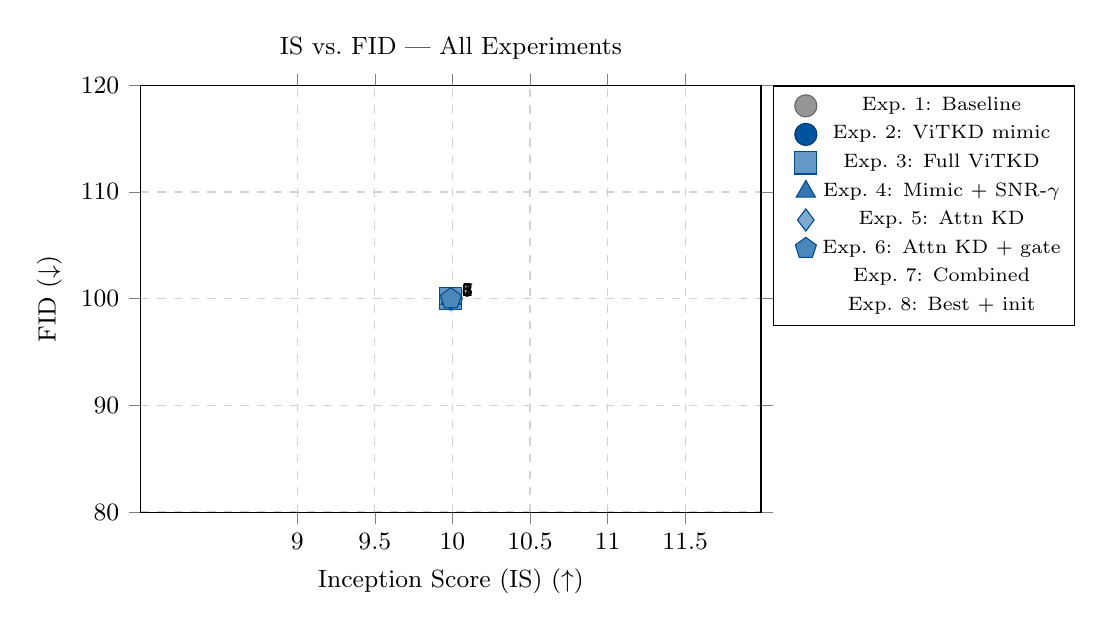
\begin{tikzpicture}
        \begin{axis}[
            width        = 0.78\linewidth,   % adjust overall plot width
            height       = 7cm,              % adjust overall plot height
            xlabel       = {Inception Score (IS) $(\uparrow)$},
            ylabel       = {FID $(\downarrow)$},
            title        = {IS vs.\ FID — All Experiments},
            grid         = both,
            grid style   = {dashed, gray!35},
            mark size    = 4pt,              % size of scatter markers in pt
            tick align   = outside,
            every axis/.append style = {font=\small},
            legend style = {
                at           = {(1.02, 1.0)}, % legend to the right of the plot
                anchor       = north west,
                font         = \scriptsize,
                legend columns = 1,
            },
            % xmin = 0, xmax = 30,   % uncomment to fix IS axis range
            % ymin = 0, ymax = 200,  % uncomment to fix FID axis range
        ]

        % -----------------------------------------------------------------
        % Each experiment is plotted as a separate \addplot so that it
        % appears individually in the legend with its own label and color.
        % To change a marker color, modify the "colorExperiment" argument
        % or replace it with any named color or \definecolor name.
        % To change the marker shape, replace "mark=*" with:
        %   mark=o          (open circle)
        %   mark=square*    (filled square)
        %   mark=triangle*  (filled triangle)
        %   mark=diamond*   (filled diamond)
        % -----------------------------------------------------------------

        \addplot[only marks, mark=*, mark options={fill=colorBaseline, draw=colorBaseline!70!black}]
            coordinates {(9.99, 99.99)};        % TODO: (IS_exp1, FID_exp1)
        \addlegendentry{Exp.\ 1: Baseline}

        \addplot[only marks, mark=*, mark options={fill=colorExperiment, draw=colorExperiment!70!black}]
            coordinates {(9.99, 99.99)};        % TODO: (IS_exp2, FID_exp2)
        \addlegendentry{Exp.\ 2: ViTKD mimic}

        \addplot[only marks, mark=square*, mark options={fill=colorExperiment!60, draw=colorExperiment!90!black}]
            coordinates {(9.99, 99.99)};        % TODO: (IS_exp3, FID_exp3)
        \addlegendentry{Exp.\ 3: Full ViTKD}

        \addplot[only marks, mark=triangle*, mark options={fill=colorExperiment!80, draw=colorExperiment!90!black}]
            coordinates {(9.99, 99.99)};        % TODO: (IS_exp4, FID_exp4)
        \addlegendentry{Exp.\ 4: Mimic + SNR-$\gamma$}

        \addplot[only marks, mark=diamond*, mark options={fill=colorExperiment!50, draw=colorExperiment!90!black}]
            coordinates {(9.99, 99.99)};        % TODO: (IS_exp5, FID_exp5)
        \addlegendentry{Exp.\ 5: Attn KD}

        \addplot[only marks, mark=pentagon*, mark options={fill=colorExperiment!70, draw=colorExperiment!90!black}]
            coordinates {(9.99, 99.99)};        % TODO: (IS_exp6, FID_exp6)
        \addlegendentry{Exp.\ 6: Attn KD + gate}

        \addplot[only marks, mark=Mercedes star*, mark options={fill=colorExperiment!90, draw=colorExperiment!90!black}]
            coordinates {(9.99, 99.99)};        % TODO: (IS_exp7, FID_exp7)
        \addlegendentry{Exp.\ 7: Combined}

        \addplot[only marks, mark=10-pointed star*, mark options={fill=red!70!black, draw=red!90!black}]
            coordinates {(9.99, 99.99)};        % TODO: (IS_exp8, FID_exp8)
        \addlegendentry{Exp.\ 8: Best + init}

        % -----------------------------------------------------------------
        % EXPERIMENT NUMBER LABELS NEXT TO EACH POINT
        % The block below places a small number label near each marker.
        % To disable all labels, delete or comment out this entire block.
        % To adjust label offset, modify the "xshift" and "yshift" values.
        % -----------------------------------------------------------------
        \node[font=\scriptsize, xshift=6pt, yshift=3pt]  at (axis cs:9.99,99.99) {1};  % TODO
        \node[font=\scriptsize, xshift=6pt, yshift=3pt]  at (axis cs:9.99,99.99) {2};  % TODO
        \node[font=\scriptsize, xshift=6pt, yshift=3pt]  at (axis cs:9.99,99.99) {3};  % TODO
        \node[font=\scriptsize, xshift=6pt, yshift=3pt]  at (axis cs:9.99,99.99) {4};  % TODO
        \node[font=\scriptsize, xshift=6pt, yshift=3pt]  at (axis cs:9.99,99.99) {5};  % TODO
        \node[font=\scriptsize, xshift=6pt, yshift=3pt]  at (axis cs:9.99,99.99) {6};  % TODO
        \node[font=\scriptsize, xshift=6pt, yshift=3pt]  at (axis cs:9.99,99.99) {7};  % TODO
        \node[font=\scriptsize, xshift=6pt, yshift=3pt]  at (axis cs:9.99,99.99) {8};  % TODO

        \end{axis}
    \end{tikzpicture}
    \caption{IS--FID scatter plot for all eight experimental configurations.
    Each point corresponds to one experiment; the upper-left region (high IS,
    low FID) indicates superior generative quality. The gray marker denotes
    the no-distillation baseline (Experiment~1); the red star marks the best
    overall result (Experiment~8).}
    \label{fig:scatter_all}
\end{figure}

The results in Table~\ref{tab:all_results} and Figure~\ref{fig:scatter_all}
collectively demonstrate that knowledge distillation consistently
[improves / modulates] the generative quality of the JiT-S/16 student
relative to training from scratch. The most substantial gains are observed
in Experiment~8, which achieves an FID of \textbf{XX.XX} and an IS of   % TODO: fill in values
\textbf{XX.XX} — a reduction of \textbf{XX.XX} FID points and an increase
of \textbf{XX.XX} IS points over the baseline. A detailed discussion of
these findings is provided in Section~\ref{sec:disc_limits}.





























































































































































\section{Discussions}
\label{sec:disc_limits}

\subsection{Interpreting the results}
\label{subsec:interp-results}

The experimental results collectively support the view that knowledge distillation provides a form of structured regularisation during student training, guiding the student’s
internal representations toward solutions that generalise more effectively to the target
data distribution.

\subsection{Limitations}
\label{subsec:limits}
Several limitations of the present framework merit acknowledgement. The
distillation loss scales $\alpha$, $\beta$, and $\gamma$ were kept at their
default values across all experiments; a systematic hyperparameter search
might yield further improvements at the cost of additional computation. The
attention timestep gate is a hard threshold, and the choice of $t_{\min}$
may be suboptimal for datasets or noise schedules that differ substantially
from those considered here. Furthermore, all experiments involve a fixed
teacher-to-student capacity ratio; the sensitivity of the framework to this
ratio, and in particular to very large capacity gaps, remains to be
characterised. Finally, although distillation incurs no additional cost at
inference time — the teacher and all distillation modules are discarded after
training — the joint forward pass through both teacher and student during
training increases per-epoch memory and compute requirements relative to
training the student from scratch.
    \part{Epilogue}
% Παραρτήματα
	%\appendices
% Βιβλιογραφία - Αναφορές
	\bibliography{references}
% Συντομογραφίες - Αρκτικόλεξα - Ακρωνύμια
	\includeabbreviations{back_matter/abbreviations}
	
%%%%%%%%%%%%%%%%%%%%%%%%%%%%%%%%%%%%%%%%%%%%%%%%%%%%
% Ευρετήριο Όρων
	\printindices
%
%%%%%%%%%%%%%%%%%%
%%%%%%%%%%%%%%%%%%

%% Δημιουργία ετικετών CD:

	\definecdlabeloffsets{0}{-0.65}{0}{0.55} % upper label x offset [cm] (default=0) /  upper label y offset [cm] (default=0) /  lower label x offset [cm] (default=0) /  lower  label y offset [cm] (default=0) -- For Q-Connect KF01579 labels use the following offset values: {0}{-0.65}{0}{0.55}

	\createcdlabel{Πρότυπο Σύστημα Ομότιμων \\ Κόμβων Βασισμένο σε Σχήματα \en{RDF}}{Κωνσταντίνος Δ. Δημητρίου}{ΟΚΤΩΒΡΙΟΣ}{2020}{8} % τίτλος διπλωματικής / όνομα συγγραφέα / μήνας / έτος / εύρος περιοχής τίτλου σε cm (προτεινόμενη τιμή: 8) 

%%σ
%% Δημιουργία εξωφύλλου θήκης CD:

	\createcdcover{Πρότυπο Σύστημα Ομότιμων \\ Κόμβων Βασισμένο σε Σχήματα \en{RDF}}{Στάμος Φ. Ευάγγελος}{ΟΚΤΩΒΡΙΟΣ}{2020}{10} % τίτλος πτυχιακής / όνομα συγγραφέα / μήνας / έτος / εύρος περιοχής τίτλου σε cm (προτεινόμενη τιμή: 10) 

%%
%
\end{document}

%%%%%%%%%%%%%%%%%%%%%%%%%%%%%%%%%%%%%%%%%%%%%%%%%%%%
